%******************** 导言区 ********************%
\documentclass[twoside]{ctexbook}
% 定义文档类型，这里统一使用中文书籍类别，即"ctexbook"

\title{《基础物理学》知识点整理}

\author{\kaishu \zihao{4}格物助航计划}
% 作者之间一定要用"\and "连接，否则名字会连到一起！

\date{2025--2026学年春季学期}


%================= 基础宏包 =================%
\usepackage{amsmath, amsthm, amssymb}      
% 数学公式核心支持
\usepackage[colorlinks, bookmarksnumbered]{hyperref} 
% 智能引用
\usepackage{tcolorbox}
% 美化定理框
\tcbuselibrary{skins, theorems, breakable} 
% 加载额外库以支持分页等更多功能
\usepackage{marginnote}                    
% 旁注系统
\usepackage[backend=biber, style=gb7714-2015]{biblatex} 
% 国标参考文献
\usepackage{booktabs}                      
% 专业表格
\usepackage{multirow}   
\usepackage{multicol}                   
% 复杂表格，合并单元格
\usepackage{tikz}
\usetikzlibrary{calc, arrows.meta, positioning}                              
% 矢量绘图
\usepackage{enumitem}                      
% 列表控制
\usepackage{balance}
% 一页多栏平衡分布
\usepackage{lscape}
% 局部版面转置，用于过宽部分的转向
\usepackage{graphicx}
% 插图
\usepackage{wrapfig}
% 文字包围图表
\usepackage{textcomp}
% 特殊符号
\usepackage{xcolor}
% 控制颜色
\usepackage{caption}
% 图表标题
\usepackage{siunitx}
% 国际单位制
\usepackage{longtable}
% 长表格
\usepackage{mathrsfs}
% 特殊字体
\usepackage{bm}
% 加粗斜体
\usetikzlibrary{calc}

%================= 页面布局 =================%
\usepackage[paper=a4paper, 
    left=3cm, right=2.5cm, 
    top=2.5cm, bottom=2.5cm, 
    marginparwidth=3cm, 
    marginparsep=0.8cm]{geometry}

%================= 定理环境 =================%
\theoremstyle{plain}
\newtheorem{theorem}{定理}[chapter]
\newtheorem{lemma}[theorem]{引理}
\newtheorem{proposition}[theorem]{命题}

\theoremstyle{definition}
\newtheorem{definition}{定义}[chapter]
\newtheorem{example}{示例}[chapter]
\newtheorem{exercise}{习题}[section]

\theoremstyle{remark}
\newtheorem*{remark}{批注}
\newtheorem*{note}{注意}
\newtheorem*{supplement}{补充}
%================= 知识框样式 =================%
\tcbuselibrary{skins, theorems}
\newtcbtheorem[auto counter, number within=chapter]{knowledge}{知识要点}%
{enhanced, colframe=blue!75, colback=blue!5, 
boxrule=1pt, arc=3mm, fonttitle=\bfseries}{th}

\newtcbtheorem[auto counter, number within=chapter]{attention}{提示}%
{enhanced, colframe=red!75!black, colback=red!5, 
boxrule=1pt, arc=3mm, fonttitle=\bfseries}{th}

%================= 智能标注系统 =================%
\newcommand{\annotate}[2][yellow]{%
    \marginnote{\textcolor{#1}{\small$\blacktriangleright$ #2}}%
}
\everymath{\displaystyle}
% 由于咱们大概率用不上引用参考文献，故不在此设置参考文献数据库

%******************** 正文 ********************%
\begin{document}



\maketitle
\clearpage
% 生成标题页
\pagenumbering{gobble}
\pagenumbering{roman}
\begin{center}
    \heiti \zihao{3}编写人员

    \kaishu \zihao{4}ccy
    \kaishu \zihao{4}fcr
    \kaishu \zihao{4}gzx
    \kaishu \zihao{4}jkw
    \kaishu \zihao{4}qjh
    \kaishu \zihao{4}szh
    \kaishu \zihao{4}xym

    （按姓名首字母排序）\\[1em]

    \heiti \zihao{3}原项目编写人员

    \kaishu \zihao{4}2415gyl
    \kaishu \zihao{4}2401syt
    \kaishu \zihao{4}2405xmy
    \kaishu \zihao{4}2415xx
    \kaishu \zihao{4}2405zjh
    \kaishu \zihao{4}2405zwj

    （按姓名首字母排序）
\end{center}

\begin{center}
    \heiti \zihao{2}符号表
    
    \kaishu \zihao{-4}
    \begin{tabular}{ccccc}
        \toprule
        量的名称&量的符号&单位名称&单位符号&量纲\\
        \midrule
        长度&$l,s$&米&$\mathrm{m}$&$\mathrm{L}$\\
        面积&$S$&平方米&$\mathrm{m^2}$&$\mathrm{L^2}$\\
        体积&$V$&立方米&$\mathrm{m^3}$&$\mathrm{L^3}$\\
        时间&$t$&秒&$\mathrm{s}$&$\mathrm{T}$\\
        位移&$\Delta r$&米&$\mathrm{m}$&$\mathrm{L}$\\
        速度&$v,u$&米每秒&$\mathrm{m/s}$&$\mathrm{LT^{-1}}$\\
        加速度&$a$&米每二次方秒&$\mathrm{m/s^2}$&$\mathrm{LT^{-2}}$\\
        角位移&$\theta$&弧度&$\mathrm{rad}$&$\mathrm{1}$\\
        角速度&$\omega$&弧度每秒&$\mathrm{rad/s}$&$\mathrm{T^{-1}}$\\
        角加速度&$\alpha$&弧度每二次方秒&$\mathrm{rad/s^2}$&$\mathrm{T^{-2}}$\\
        质量&$m$&千克&$\mathrm{kg}$&$\mathrm{M}$\\
        力&$F$&牛顿&$\mathrm{N}$&$\mathrm{LMT^{-2}}$\\
        重力&$G$&牛顿&$\mathrm{N}$&$\mathrm{LMT^{-2}}$\\
        功&$A$&焦耳&$\mathrm{J}$&$\mathrm{L^2MT^{-2}}$\\
        能量&$E$&焦耳&$\mathrm{J}$&$\mathrm{L^2MT^{-2}}$\\
        动能&$E_k$&焦耳&$\mathrm{J}$&$\mathrm{L^2MT^{-2}}$\\
        势能&$E_p$&焦耳&$\mathrm{J}$&$\mathrm{L^2MT^{-2}}$\\
        功率&$P$&瓦特&$\mathrm{W}$&$\mathrm{L^2MT^{-3}}$\\
        摩擦因数&$\mu $&$\mathrm{-}$&$\mathrm{-}$&1\\
        动量&$p$&千克米每秒&$\mathrm{kg\cdot m/s}$&$\mathrm{LMT^{-1}}$\\
        冲量&$I$&牛顿秒&$\mathrm{N\cdot s}$&$\mathrm{LMT^{-1}}$\\
        力矩&$M$&牛顿米&$\mathrm{N\cdot m}$&$\mathrm{L^2MT^{-2}}$\\
        转动惯量&$J$&千克二次方米&$\mathrm{kg\cdot m^2}$&$\mathrm{L^2M}$\\
        角动量（动量矩）&$L$&千克二次方米每秒&$\mathrm{kg\cdot m^2/s}$&$\mathrm{L^2MT^{-1}}$\\
        压强&$p$&帕斯卡&$\mathrm{Pa}$&$\mathrm{L^{-1}MT^{-2}}$\\
        热力学温度&$T$&开尔文&$\mathrm{K}$&$\Theta$\\
        摄氏温度&$t$&摄氏度&\textcelsius&$\Theta$\\
        摩尔质量&$M$&千克每摩尔&$\mathrm{kg/mol}$&$\mathrm{MN^{-1}}$\\
        分子质量&$m_0$&千克&$\mathrm{kg}$&$\mathrm{M}$\\
        分子有效直径&$d$&米&$\mathrm{m}$&$\mathrm{L}$\\
        \bottomrule
        
        
    \end{tabular}

    \newpage
    \begin{tabular}{ccccc}
        \toprule
        量的名称&量的符号&单位名称&单位符号&量纲\\
        \midrule
        分子平均自由程&$\bar{\lambda}$&米&$\mathrm{m}$&$\mathrm{L}$\\
        分子平均碰撞频率&$\bar{Z}$&次每秒&$\mathrm{s^{-1}}$&$\mathrm{T^{-1}}$\\
        体积分子数&$n$&每立方米&$\mathrm{m^{-3}}$&$\mathrm{L^{-3}}$\\
        热量&$Q$&焦耳&$\mathrm{J}$&$\mathrm{L^2MT^{-3}}$\\
        

        比热容&$c$&焦耳每千克开尔文&$\mathrm{J/(kg\cdot K)}$&$\mathrm{L^2T^{-2}}\Theta^{-1}$\\
        热容&$C$&焦耳每开尔文&$\mathrm{J/K}$&$\mathrm{L^2MT^{-2}}\Theta^{-1}$\\
       

        摩尔定容比热容&$C_{V,m}$&焦耳每摩尔开尔文&$\mathrm{J/(mol\cdot K)}$&$\mathrm{L^2MT^{-2}N^{-1}}\Theta^{-1}$\\
        
        摩尔定压比热容&$C_{p,m}$&焦耳每摩尔开尔文&$\mathrm{J/(mol\cdot K)}$&$\mathrm{L^2MT^{-2}N^{-1}}\Theta^{-1}$\\

        比热容比&$\gamma$&$\mathrm{-}$&$\mathrm{-}$&1\\
        粘度&$\eta$&帕秒&$\mathrm{Pa\cdot s}$&$\mathrm{L^{-1}MT^{-1}}$\\
        热导率&$\kappa$&瓦每米开尔文&$\mathrm{W/(m\cdot K)}$&$\mathrm{LMT^{-3}}\Theta^{-1}$\\
        扩散系数&$D$&二次方米每秒&$\mathrm{m^2/s}$&$\mathrm{L^2T^{-1}}$\\
        熵&$S$&焦耳每开尔文&$\mathrm{J/K}$&$\mathrm{L^2MT^{-2}}\Theta^{-1}$\\
        电流&$I$&安培&$\mathrm{A}$&$\mathrm{I}$\\
        电荷量&$Q,q$&库仑&$\mathrm{C}$&$\mathrm{TI}$\\
        电荷线密度&$\lambda$&库仑每米&$\mathrm{C/m}$&$\mathrm{L^{-1}TI}$\\
        电荷面密度&$\sigma$&库仑每平方米&$\mathrm{C/m^2}$&$\mathrm{L^{-2}TI}$\\
        电荷体密度&$\rho$&库仑每立方米&$\mathrm{C/m^3}$&$\mathrm{L^{-3}TI}$\\
        电场强度&$E$&伏特每米&$\mathrm{V/m\text{或}N/C}$&$\mathrm{LMT^{-3}I^{-1}}$\\
        电场强度通量&$\Phi_e$&库仑&$\mathrm{C}$&$\mathrm{TI}$\\
        电势&$V$&伏特&$\mathrm{V}$&$\mathrm{L^2MT^{-3}I^{-1}}$\\
        电势差（电压）&$U$&伏特&$\mathrm{V}$&$\mathrm{L^2MT^{-3}I^{-1}}$\\
        电容率&$\epsilon$&法拉每米&$\mathrm{F/m}$&$\mathrm{L^{-3}M^{-1}T^4I^2}$\\

        真空电容率&$\epsilon_0$&法拉每米&$\mathrm{F/m}$&$\mathrm{L^{-3}M^{-1}T^4I^2}$\\
        相对电容率&$\epsilon_r$&$\mathrm{-}$&$\mathrm{-}$&1\\
        电偶极矩&$p,p_e$&库仑米&$\mathrm{C\cdot m}$&$\mathrm{LTI}$\\
        电极化强度&$P$&库仑每平方米&$\mathrm{C/m^2}$&$\mathrm{L^{-2}TI}$\\
        电极化率&$\chi_e$&$\mathrm{-}$&$\mathrm{-}$&1\\
        电位移&$D$&库仑每平方米&$\mathrm{C/m^2}$&$\mathrm{L^{-2}TI}$\\
        电位移通量&$\Psi$&库仑&$\mathrm{C}$&$\mathrm{TI}$\\
        电容&$C$&法拉&$\mathrm{F}$&$\mathrm{L^{-2}M^{-1}T^{4}I^2}$\\
        电流密度&$j$&安培每平方米&$\mathrm{A/m^2}$&$\mathrm{L^{-2}I}$\\
        电动势&$\mathscr{E}$&伏特&$\mathrm{V}$&$\mathrm{L^2MT^{-3}I^{-1}}$\\
        电阻&$R$&欧姆&$\Omega$&$\mathrm{L^2MT^{-3}I^{-2}}$\\
        
        \bottomrule
    \end{tabular}
        
    \newpage
    \begin{tabular}{ccccc}
        \toprule
        量的名称&量的符号&单位名称&单位符号&量纲\\
        \midrule
        电导&$G$&西门子&$\mathrm{S}$&$\mathrm{L^{-2}M^{-1}T^3I^2}$\\
        电阻率&$\rho$&欧姆米&$\Omega\mathrm{\cdot m}$&$\mathrm{L^3MT^{-3}I^{-2}}$\\
        电导率&$\gamma$&西门子每米&$\mathrm{S/m}$&$\mathrm{L^{-3}M^{-1}T^3I^2}$\\
        磁感应强度&$B$&特斯拉&$\mathrm{T}$&$\mathrm{MT^{-2}I^{-1}}$\\
        磁导率&$\mu$&亨利每米&$\mathrm{H/m}$&$\mathrm{LMT^{-2}I^{-2}}$\\
        真空磁导率&$\mu_0$&亨利每米&$\mathrm{H/m}$&$\mathrm{LMT^{-2}I^{-2}}$\\
        相对磁导率&$\mu_r$&$\mathrm{-}$&$\mathrm{-}$&1\\
        磁通量&$\Phi$&韦伯&$\mathrm{Wb}$&$\mathrm{L^2MT^{-2}I^{-1}}$\\
        磁化强度&$M$&安培每米&$\mathrm{A/m}$&$\mathrm{L^{-1}I}$\\
        磁化率&$\chi_m$&$\mathrm{-}$&$\mathrm{-}$&1\\
        磁场强度&$H$&安培每米&$\mathrm{A/m}$&$\mathrm{L^{-1}I}$\\
        （线圈的）磁矩&$m$&安培平方米&$\mathrm{A\cdot m^2}$&$\mathrm{L^2I}$\\
        自感&$L$&亨利&$\mathrm{H}$&$\mathrm{L^2MT^{-2}I^{-2}}$\\
        互感&$M$&亨利&$\mathrm{H}$&$\mathrm{L^2MT^{-2}I^{-2}}$\\
        电场能量&$W_e$&焦耳&$\mathrm{J}$&$\mathrm{L^2MT^{-2}}$\\
        磁场能量&$W_m$&焦耳&$\mathrm{J}$&$\mathrm{L^2MT^{-2}}$\\
        电磁能密度&$\omega$&焦耳每立方米&$\mathrm{J/m^3}$&$\mathrm{L^{-1}MT^{-2}}$\\
        \bottomrule
    \end{tabular}
\end{center}



\tableofcontents

\cleardoublepage

\pagenumbering{arabic}
\documentclass[a4paper,12pt]{ctexart}
\usepackage{geometry}
\usepackage{amsmath}
\usepackage{amssymb}
\usepackage{enumitem}
\usepackage{booktabs}
\usepackage{tikz}
\usetikzlibrary{arrows.meta}

% 页面设置
\geometry{left=2.5cm, right=2.5cm, top=2.5cm, bottom=2.5cm}
\linespread{1.25}

% 全局首行缩进
\setlength{\parindent}{2em}
\setlength{\parskip}{0.3em}

% 列表设置
\setlist{
    leftmargin=2em,
    itemindent=0em,
    labelindent=0em,
    topsep=0.3em,
    itemsep=0.1em
}

% 矢量
\newcommand{\vct}[1]{\boldsymbol{#1}}
\newcommand{\uve}[1]{\boldsymbol{\hat{#1}}}

\title{格物助航计划\\质点运动学基础知识点提纲}
\author{北航工科物理资料整理组}
\date{\today}

\begin{document}

\maketitle

\vspace{1em}

\tableofcontents
\newpage

\section{第一章：质点运动学}

\subsection{章节主线与学习目标}
本章的核心任务是建立描述机械运动的定量语言，不涉及运动变化的原因。本部分（1.1-1.5）按照"描述前提-理想模型-数学工具-基本物理量"的逻辑展开：
\[
\text{时空观} \rightarrow \text{质点模型} \rightarrow \text{参考系与坐标系} \rightarrow \text{位置描述} \rightarrow \text{运动快慢描述}
\]

通过本部分学习，读者应具备以下核心能力：
\begin{enumerate}[label=\arabic*.]
\item 能够独立建立描述运动的完整坐标系，明确所有约定条件；
\item 能够准确判断任意物理场景下质点模型的适用性；
\item 能够熟练写出直角坐标系下质点的运动方程，并推导其轨道方程；
\item 能够严格区分矢量与标量物理量，正确计算位移、速度和速率。
\end{enumerate}

\subsection{时间与空间}
\textbf{重点学习}
\begin{enumerate}
\item 机械运动的本质是物体的空间位置随时间的变化，时间和空间是描述运动的两个基本维度。
\item 经典力学的时空观：时间和空间是绝对的、均匀的、各向同性的。时间均匀流逝，与参考系无关；空间是平坦的欧几里得空间，长度测量与参考系无关。
\item 参考系：为了确定物体的位置和描述其运动而选作标准的物体或物体系。运动的描述具有相对性，同一物体在不同参考系中的运动形式可能完全不同。
\item 坐标系：固结在参考系上的数学标架，由原点和一组正交单位矢量组成，用于将物体的位置量化为数值坐标。坐标系是参考系的数学抽象，同一参考系可以选择不同的坐标系。
\item 国际单位制（SI）：力学的三个基本物理量及其单位为：长度（米，m）、时间（秒，s）、质量（千克，kg）。所有力学量都可以由这三个基本量导出，量纲分析是检验物理公式正确性的重要方法。
\end{enumerate}

\textbf{常见误区}
\begin{itemize}
\item 认为参考系必须是静止的：参考系可以任意选择，通常选择使问题简化的参考系；
\item 混淆参考系和坐标系：参考系是实物，坐标系是数学工具，二者不能等同；
\item 忽略量纲检查：所有物理公式两边的量纲必须一致，量纲错误的公式一定是错误的。
\end{itemize}

\textbf{基础量纲分析入门}

量纲是物理量的基本属性，用于表示物理量与基本物理量之间的导出关系。在力学中，国际单位制的三个基本量纲为：长度$[L]$、时间$[T]$、质量$[M]$。任意力学量$A$的量纲均可表示为幂次组合形式：
\[
[A] = L^\alpha T^\beta M^\gamma
\]
其中$\alpha,\beta,\gamma$为量纲指数。

\textbf{量纲分析的核心作用}：
\begin{enumerate}[label=(\arabic*)]
\item 快速检验物理公式的正确性（量纲不一致的公式必然错误）；
\item 推导未知物理量的量纲，进而确定其国际单位；
\item 辅助建立物理量之间的定性关系。
\end{enumerate}

\textbf{重要提示}：量纲正确是公式成立的必要条件，而非充分条件。

\textbf{运动学量纲分析例题}
某同学推导匀变速直线运动的位移公式时得到了以下三个表达式，其中$x$为位移，$v_0$为初速度，$a$为加速度，$t$为运动时间。请用量纲分析判断哪个表达式一定是错误的：
\begin{enumerate}[label=(\Alph*)]
\item $x = v_0 t + \frac{1}{2} a t^2$
\item $x = v_0 t + a t$
\item $x = \frac{1}{2} a t^2$
\end{enumerate}

\textbf{解析}：
分别计算等式两边各项的量纲：
\begin{itemize}
\item 位移$x$的量纲：$[x] = L$
\item 速度$v_0$的量纲：$[v_0] = L T^{-1}$，因此$[v_0 t] = L T^{-1} \cdot T = L$
\item 加速度$a$的量纲：$[a] = L T^{-2}$，因此$[a t^2] = L T^{-2} \cdot T^2 = L$，$[a t] = L T^{-2} \cdot T = L T^{-1}$
\end{itemize}
选项B中，$v_0 t$的量纲为$L$，而$a t$的量纲为$L T^{-1}$，两项量纲不一致，不能进行代数相加，因此该表达式一定是错误的。

量纲分析是贯穿整个物理学的通用方法，其适用范围远不止力学领域。在电磁学、热学、光学、原子物理等所有物理分支中，所有物理量的量纲都可以由国际单位制（SI）规定的七个基本量纲导出。任意物理量$A$的通用量纲表达式为：
\[
[A] = L^\alpha T^\beta M^\gamma I^\delta \Theta^\varepsilon N^\zeta J^\eta
\]
其中$I$为电流的量纲，$\Theta$为热力学温度的量纲，$N$为物质的量的量纲，$J$为发光强度的量纲，$\alpha,\beta,\gamma,\delta,\varepsilon,\zeta,\eta$为对应的量纲指数。

\begin{table}[htbp]
  \centering
  \caption{国际单位制（SI）基本量纲与基本单位（2019年修订版）}
  \begin{tabular}{cccc}
    \toprule
    基本量纲 & 物理量名称 & 基本单位名称 & 单位符号 \\
    \midrule
    $L$ & 长度 & 米 & m \\
    $T$ & 时间 & 秒 & s \\
    $M$ & 质量 & 千克 & kg \\
    $I$ & 电流 & 安培 & A \\
    $\Theta$ & 热力学温度 & 开尔文 & K \\
    $N$ & 物质的量 & 摩尔 & mol \\
    $J$ & 发光强度 & 坎德拉 & cd \\
    \bottomrule
  \end{tabular}
  \label{tab:si_basic_units}
\end{table}

注：国际单位制中还包含弧度（rad）和球面度（sr）两个辅助单位，用于表示平面角和立体角，其量纲为1（无量纲）。

\textbf{理论力学衔接}

经典力学的时空观是整个牛顿力学的基础。在理论力学中，我们将进一步引入"构型空间"的概念，物体的所有可能位置构成一个多维空间，每个点对应物体的一个构型。

\subsection{物体的点模型：质点}
\textbf{重点学习}
\begin{enumerate}[label=\arabic*.]
\item 质点是力学中最基本的理想模型，定义为具有一定质量但几何尺寸可以忽略不计的物体。
\item 理想模型的意义：抓住问题的主要矛盾，忽略次要因素，使复杂的物理问题得以简化。
\item 质点模型的适用条件：当物体的大小和形状对所研究问题的影响可以忽略不计时，即可将物体视为质点。具体包括两种情况：
    \begin{enumerate}[label=(\alph*)]
    \item 物体的线度远小于研究问题中涉及的距离；
    \item 物体只做平动，不发生转动或形变。
    \end{enumerate}
\item 一个物体能否视为质点，完全取决于所研究的问题，与物体本身的大小无关。
\end{enumerate}

\textbf{常见误区}
\begin{itemize}
\item 认为小物体一定能视为质点，大物体一定不能视为质点：例如，研究原子的内部结构时，原子不能视为质点；研究地球绕太阳的公转时，地球可以视为质点；
\item 认为质点就是几何点：质点具有质量，而几何点没有质量；
\item 不考虑研究问题，笼统地说某个物体是质点。
\end{itemize}

\textbf{理论力学衔接}


质点模型是单自由度系统的最简单情况。在理论力学中，我们将研究更复杂的模型，如质点系（多个质点组成的系统）和刚体（形状和大小不变的物体）。刚体可以看作是质点系的一种特例，即刚体可以视作质点之间无相对位移的质点系。刚体的引入是理论力学学习的非常重要的内容，也是由理论迈向实际的关键一环。

刚体是由无数个质点组成、且任意两质点间距离保持不变的理想模型。对于自由刚体，除了需要3个坐标确定其质心的平动位置外，还需要3个独立的转角坐标（通常称为欧拉角）确定其在空间中的取向，因此自由刚体总共具有6个自由度：3个平动自由度 + 3个转动自由度。这也解释了质点模型的本质：当物体的转动和形变对所研究问题的影响可以忽略时，我们实际上是将6个自由度的刚体简化为仅具有3个平动自由度的质点，从而极大地简化了问题。

刚体自由度的概念在工程领域有极其广泛的应用：例如航空航天中卫星的姿态控制，本质上就是通过推力器和飞轮精确控制卫星的3个转动自由度（俯仰、偏航、滚转）；机械工程中的工业机器人，每个关节通常对应一个自由度，通过多个关节的组合实现末端执行器的任意位姿；而在研究车辆的平面运动时，我们通常只考虑3个自由度（质心的x、y坐标和车身的转角），并通过轮胎的约束条件进一步简化问题。在理论力学中，我们还将进一步学习约束对自由度的影响，以及如何使用广义坐标来描述具有任意自由度的力学系统。

\subsection{位置矢量与轨道方程}
\textbf{重点学习}
\begin{enumerate}[label=\arabic*.]
\item 位置矢量（位矢）：从坐标系原点指向质点所在位置的矢量，记为$\vct{r}$。位矢同时给出了质点到原点的距离和相对于原点的方位。
\item 直角坐标系中的位矢表示：
\[
\vct{r}(t) = x(t)\uve{i} + y(t)\uve{j} + z(t)\uve{k}
\]
其中$\uve{i},\uve{j},\uve{k}$分别为x、y、z轴正方向的单位矢量，$x(t),y(t),z(t)$为质点在三个坐标轴上的坐标，都是时间$t$的函数。
\item 运动方程：描述质点位置随时间变化规律的方程，其矢量形式为$\vct{r}=\vct{r}(t)$，分量形式为$x=x(t),y=y(t),z=z(t)$。运动方程包含了质点运动的全部信息。
\item 轨道方程：描述质点在空间中运动轨迹的几何方程。由运动方程的分量形式消去时间参数$t$，即可得到轨道方程$f(x,y,z)=0$。
\end{enumerate}

\textbf{常用坐标系及其位矢表示}
坐标系是描述质点位置的数学工具，选择合适的坐标系可以极大简化问题的求解。在运动学中，最常用的三种坐标系为笛卡尔坐标系、平面极坐标系和自然坐标系。

\subsubsection{笛卡尔坐标系（直角坐标系）}
笛卡尔坐标系是最基础、最通用的坐标系，由三条相互垂直的坐标轴组成。
\begin{itemize}
\item \textbf{定义}：以空间中某点$O$为原点，建立三条相互垂直的坐标轴$x$、$y$、$z$，分别对应三个正交单位矢量$\uve{i}$、$\uve{j}$、$\uve{k}$。
\item \textbf{适用情况}：绝大多数直线运动、直角坐标系下的曲线运动（如抛体运动）、以及没有明显对称性的一般运动。
\item \textbf{位矢表示}：
\[
\vct{r} = x\uve{i} + y\uve{j} + z\uve{k}
\]
\end{itemize}

\begin{figure}[htbp]
  \centering
  \begin{tikzpicture}[scale=1.2, >=Stealth]
    \draw[->] (0,0,0) -- (3,0,0) node[right] {$x$};
    \draw[->] (0,0,0) -- (0,3,0) node[above] {$y$};
    \draw[->] (0,0,0) -- (0,0,3) node[below left] {$z$};
    \draw[->, thick, blue] (0,0,0) -- (2,2,1) node[above right] {$\vct{r}$};
    \draw[dashed] (2,2,1) -- (2,2,0) -- (2,0,0);
    \draw[dashed] (2,2,0) -- (0,2,0);
    \node at (2.2,0,0) {$x$};
    \node at (0,2.2,0) {$y$};
    \node at (0,0,1.2) {$z$};
    \node at (1.5,0,0) {$\uve{i}$};
    \node at (0,1.5,0) {$\uve{j}$};
    \node at (0,0,1.5) {$\uve{k}$};
  \end{tikzpicture}
  \caption{笛卡尔坐标系与位矢}
\end{figure}

\subsubsection{平面极坐标系}
平面极坐标系适用于描述平面内具有径向对称性的运动。
\begin{itemize}
\item \textbf{定义}：以平面内某点$O$为原点，建立水平极轴。质点的位置由极径$r$（原点到质点的距离）和极角$\theta$（极轴到位矢的夹角）确定，对应两个正交单位矢量$\uve{e}_r$（径向，沿位矢 outward）和$\uve{e}_\theta$（角向，垂直于$\uve{e}_r$逆时针方向）。
\item \textbf{适用情况}：径向运动、圆周运动、中心力问题（如行星绕太阳的运动、卫星轨道）。
\item \textbf{位矢表示}：
\[
\vct{r} = r\uve{e}_r
\]
注意：极坐标中的单位矢量$\uve{e}_r$和$\uve{e}_\theta$是随质点位置变化的，这是与笛卡尔坐标系的本质区别。
\end{itemize}

\begin{figure}[htbp]
  \centering
  \begin{tikzpicture}[scale=1.5, >=Stealth]
    \draw[->] (-1,0) -- (3,0) node[right] {};
    \node at (3.1,0) {极轴};
    \node at (-0.2,-0.2) {$O$};
    \draw[->, thick, blue] (0,0) -- (45:2) node[above right] {$\vct{r} = r\uve{e}_r$};
    \node at (45:1) {$r$};
    \draw (0.5,0) arc(0:45:0.5) node[midway, above right] {$\theta$};
    \draw[->, thick, red] (45:2) -- (45:2.7) node[above right] {$\uve{e}_r$};
    \draw[->, thick, green] (45:2) -- (135:2.7) node[above left] {$\uve{e}_\theta$};
  \end{tikzpicture}
  \caption{平面极坐标系与位矢}
\end{figure}

\subsubsection{自然坐标系}
自然坐标系是沿质点运动轨迹建立的坐标系，特别适合描述已知轨迹的曲线运动，采用圆形轨迹演示最为直观。
\begin{itemize}
\item \textbf{定义}：在质点的运动轨迹上任选一点$O$为原点，规定轨迹的正方向，用弧长$s$表示质点的位置。在质点所在位置建立两个正交单位矢量：切向单位矢量$\uve{\tau}$（沿轨迹切线指向运动正方向）和法向单位矢量$\uve{n}$（沿轨迹法线指向凹侧，对于圆周运动即指向圆心）。
\item \textbf{适用情况}：已知轨迹的曲线运动（如圆周运动、摆线运动、车辆沿道路的运动）。
\item \textbf{位矢表示}：
\[
\vct{r} = \vct{r}(s)
\]
其中$s$为质点到原点$O$的弧长，是时间$t$的函数$s=s(t)$。
\end{itemize}

\begin{figure}[htbp]
  \centering
  \begin{tikzpicture}[scale=1.2, >=Stealth]
    \draw[thick] (0,0) circle (2);
    \node at (0,2.2) {轨迹正方向};
    \draw[->] (120:2) arc(120:90:2);
    \fill (2,0) circle (2pt) node[below right] {$O$};
    \fill (45:2) circle (2pt) node[above right] {$P$};
    \draw[->] (2,0) arc(0:45:2) node[midway, above right] {$s$};
    \draw[->, thick, red] (45:2) -- (135:2.7) node[above left] {$\uve{\tau}$};
    \draw[->, thick, green] (45:2) -- (45:1.3) node[below left] {$\uve{n}$};
  \end{tikzpicture}
  \caption{自然坐标系与位矢（圆形轨迹）}
\end{figure}

\textbf{常见误区}
\begin{itemize}
\item 混淆运动方程和轨道方程：运动方程是时间的函数，描述质点在任意时刻的位置；轨道方程是几何关系，只描述质点运动的轨迹形状，不包含时间信息；
\item 消去时间参数时忽略参数的取值范围，导致轨道方程的定义域错误；
\item 认为位矢的大小就是质点的位移：位矢是从原点指向质点的矢量，位移是质点在一段时间内位置的变化量。
\end{itemize}

\textbf{理论力学衔接}

在理论力学中，我们将引入广义坐标的概念。广义坐标是能够唯一确定系统构型的一组独立变量，不一定是直角坐标。例如，对于在平面上运动的质点，可以用极坐标$(r,\theta)$作为广义坐标。

\subsection{速度矢量}

\subsubsection{速度矢量的基础定义}
速度是描述质点运动快慢和方向的物理量，是矢量。为了准确理解速度的概念，我们首先明确以下几个基本物理量：

\textbf{位移}：质点在一段时间内位置的变化量，是矢量。设质点在$t$时刻的位矢为$\vct{r}(t)$，在$t+\Delta t$时刻的位矢为$\vct{r}(t+\Delta t)$，则在$\Delta t$时间内的位移为：
\[
\Delta\vct{r} = \vct{r}(t+\Delta t) - \vct{r}(t)
\]
位移的大小是质点初末位置之间的直线距离，方向由初位置指向末位置。

\textbf{路程}：质点在一段时间内实际运动轨迹的长度，是标量。一般情况下，位移的大小$|\Delta\vct{r}|$不等于路程$\Delta s$，只有当质点做单向直线运动时，二者才相等。

\textbf{平均速度}：位移与发生这段位移所用时间的比值，是矢量：
\[
\overline{\vct{v}} = \frac{\Delta\vct{r}}{\Delta t}
\]
平均速度的方向与位移方向相同，它只能粗略地描述质点在一段时间内的平均运动状态。

\textbf{瞬时速度（简称速度）}：平均速度在$\Delta t \to 0$时的极限，即位矢对时间的一阶导数：
\[
\vct{v} = \lim_{\Delta t \to 0} \frac{\Delta\vct{r}}{\Delta t} = \frac{d\vct{r}}{dt}
\]
速度是矢量，其方向沿质点运动轨迹的切线方向，指向运动的前方。

\textbf{速率}：速度的大小，是标量：
\[
v = |\vct{v}| = \left| \frac{d\vct{r}}{dt} \right| = \frac{ds}{dt}
\]
其中$s$为质点运动的路程。速率等于路程对时间的变化率，它只描述质点运动的快慢，不涉及方向。

\subsubsection{不同坐标系下的速度矢量}
速度矢量的表达式与坐标系的选择密切相关。基于前一节介绍的三种常用坐标系，我们分别推导速度的分量形式。

\textbf{1. 笛卡尔坐标系（直角坐标系）}
在笛卡尔坐标系中，单位矢量$\uve{i},\uve{j},\uve{k}$是恒定不变的，因此速度的推导最为简单。将位矢$\vct{r}=x\uve{i}+y\uve{j}+z\uve{k}$对时间求导：
\[
\vct{v} = \frac{d\vct{r}}{dt} = \frac{dx}{dt}\uve{i} + \frac{dy}{dt}\uve{j} + \frac{dz}{dt}\uve{k} = v_x\uve{i} + v_y\uve{j} + v_z\uve{k}
\]
其中$v_x=\frac{dx}{dt},v_y=\frac{dy}{dt},v_z=\frac{dz}{dt}$分别为速度在三个坐标轴上的分量。速度的大小为：
\[
v = \sqrt{v_x^2 + v_y^2 + v_z^2}
\]

\textbf{2. 平面极坐标系}
在平面极坐标系中，位矢表示为$\vct{r}=r\uve{e}_r$。与笛卡尔坐标系不同，极坐标的单位矢量$\uve{e}_r$和$\uve{e}_\theta$是随质点位置变化的，因此求导时必须考虑单位矢量本身的变化：
\[
\vct{v} = \frac{d\vct{r}}{dt} = \frac{dr}{dt}\uve{e}_r + r\frac{d\uve{e}_r}{dt}
\]
通过几何分析可以证明，径向单位矢量的导数为$\frac{d\uve{e}_r}{dt}=\frac{d\theta}{dt}\uve{e}_\theta$，代入上式得到极坐标系下的速度表达式：
\[
\vct{v} = \dot{r}\uve{e}_r + r\dot{\theta}\uve{e}_\theta = v_r\uve{e}_r + v_\theta\uve{e}_\theta
\]
其中$v_r=\dot{r}$称为径向速度，描述质点到原点距离的变化率；$v_\theta=r\dot{\theta}$称为角向速度（或横向速度），描述质点方位角的变化率。

\textbf{3. 自然坐标系}
在自然坐标系中，质点的位置由弧长$s$表示，位矢为$\vct{r}=\vct{r}(s)$。根据复合函数求导法则：
\[
\vct{v} = \frac{d\vct{r}}{dt} = \frac{d\vct{r}}{ds} \cdot \frac{ds}{dt}
\]
其中$\frac{d\vct{r}}{ds}$的大小为1，方向沿轨迹切线方向，即切向单位矢量$\uve{\tau}$。因此自然坐标系下的速度表达式为：
\[
\vct{v} = v\uve{\tau} = \frac{ds}{dt}\uve{\tau}
\]
自然坐标系下的速度只有切向分量，这是其最显著的特点。

\subsubsection{矢量求导的物理意义}
矢量求导是运动学中最核心的数学工具，它与标量求导有着本质的区别：
- 标量的导数只描述其大小的变化率
- 矢量的导数同时描述其大小的变化率和方向的变化率

对于任意矢量$\vct{A}(t)$，其导数可以分解为两部分：
\[
\frac{d\vct{A}}{dt} = \frac{dA}{dt}\uve{e}_A + A\frac{d\uve{e}_A}{dt}
\]
其中第一项$\frac{dA}{dt}\uve{e}_A$描述矢量大小的变化，第二项$A\frac{d\uve{e}_A}{dt}$描述矢量方向的变化。

在运动学中，这一区别至关重要：
- 当质点做直线运动时，速度方向不变，只有大小变化，因此加速度只改变速度大小
- 当质点做曲线运动时，速度方向不断变化，即使速度大小不变，也存在加速度（如匀速圆周运动）

矢量求导的思想贯穿整个力学课程，是后续学习加速度、角动量等物理量的基础。

\subsubsection{典型例题：匀速圆周运动的速度分析}
为了直观说明速度的矢量性，我们以匀速圆周运动为例进行分析。设质点在半径为$R$的圆周上以恒定的速率$v$运动，$t=0$时质点位于x轴正方向。

\textbf{方法一：笛卡尔坐标系}
质点的运动方程为：
\[
x = R\cos\omega t, \quad y = R\sin\omega t
\]
其中$\omega=\frac{v}{R}$为角速度。对时间求导得到速度分量：
\[
v_x = \frac{dx}{dt} = -R\omega\sin\omega t, \quad v_y = \frac{dy}{dt} = R\omega\cos\omega t
\]
速度的大小为：
\[
v = \sqrt{v_x^2 + v_y^2} = R\omega = \text{常量}
\]
速度的方向由方向角$\alpha$确定：
\[
\tan\alpha = \frac{v_y}{v_x} = -\cot\omega t = \tan\left(\omega t + \frac{\pi}{2}\right)
\]
可见速度方向始终与位矢方向垂直，即沿圆周切线方向。

\textbf{方法二：极坐标系}
在极坐标系中，$r=R=\text{常量}$，$\theta=\omega t$。代入极坐标速度公式：
\[
v_r = \dot{r} = 0, \quad v_\theta = r\dot{\theta} = R\omega = v
\]
因此速度只有角向分量，大小为$v$，方向沿圆周切线方向，与笛卡尔坐标系结果一致。

\textbf{结论}：匀速圆周运动的速度大小保持不变，但方向不断变化，因此它是一种变速运动，必然存在加速度。这一结论充分体现了速度的矢量性。

\textbf{常见误区}
\begin{itemize}
\item 混淆位移和路程：位移是矢量，路程是标量；
\item 混淆平均速度和平均速率：平均速率是路程与时间的比值，是标量；平均速度的大小是位移大小与时间的比值，一般不等于平均速率；
\item 认为速度的方向总是与位矢的方向相同：速度方向沿轨迹切线方向，与位矢方向无关；
\item 认为速度的大小不变时，速度就不变：速度是矢量，大小和方向只要有一个发生变化，速度就发生变化；
\item 忽略极坐标和自然坐标系中单位矢量的变化，求导时只对分量求导而不对单位矢量求导。
\end{itemize}

\textbf{理论力学衔接}

速度是描述质点运动状态的基本物理量之一。在理论力学中，我们将看到，质点的运动状态由其位置和速度共同决定。哈密顿力学则进一步引入动量作为基本变量，建立了更普适的力学体系。对于刚体的运动，我们还将引入角速度矢量来描述其转动状态。

\end{document}
\section{加速度矢量}
\subsection{核心内容}
\begin{enumerate}
    \item \textbf{定义}：加速度矢量是速度矢量对时间的导数，即位矢对时间的二阶导数。
          \[
              \vec{a} = \lim_{\Delta t \to 0} \frac{\Delta \vec{v}}{\Delta t} = \frac{d\vec{v}}{dt} = \frac{d^2 \vec{r}}{dt^2}.
          \]
    \item \textbf{物理意义}：加速度既可改变速度的大小，也可改变速度的方向。
    \item \textbf{曲线运动特征}：一般情况下，加速度指向轨迹的凹侧（速度矢量方向与加速度矢量方向之间夹着轨迹）。
    \item \textbf{直角坐标系分解}：
          \[
              \vec{v} = \dot{x}\,\vec{i} + \dot{y}\,\vec{j} + \dot{z}\,\vec{k},\quad
              \vec{a} = \ddot{x}\,\vec{i} + \ddot{y}\,\vec{j} + \ddot{z}\,\vec{k}.
          \]
\end{enumerate}

\subsection{常见误区与澄清}
\begin{itemize}
    \item \textbf{误区}：混淆“加速度大小”与“速率变化率”。\\
          \textbf{澄清}：加速度大小 $|\vec{a}|$ 反映的是速度矢量变化的快慢。如在变速圆周运动中，速率变化率仅为切向加速度 $a_\tau = \frac{dv}{dt}$。
\end{itemize}

\subsection{例题}
\textbf{题目}：已知质点运动方程为：
\[
    x(t) = R(\omega t - \sin\omega t),\quad y(t) = R(1 - \cos\omega t),
\]
求 $t = \frac{\pi}{\omega}$ 时的速度与加速度。\\

\textbf{解法}：
\begin{enumerate}
    \item 先求导：
          \[
              v_x = R\omega(1 - \cos\omega t),\quad v_y = R\omega\sin\omega t;
          \]
          \[
              a_x = R\omega^2\sin\omega t,\quad a_y = R\omega^2\cos\omega t.
          \]
    \item 代入 $t = \frac{\pi}{\omega}$：
          \[
              v_x = 2R\omega,\ v_y = 0;\quad a_x = 0,\ a_y = -R\omega^2.
          \]
\end{enumerate}

\newpage

\section{运动学中的逆问题}
\subsection{核心内容}
\begin{enumerate}
    \item \textbf{正问题}：已知 $\vec{r}(t)$，求 $\vec{v}(t), \vec{a}(t)$（求导）。
    \item \textbf{逆问题}：已知 $\vec{a}(t)$ 与初始条件，求 $\vec{v}(t), \vec{r}(t)$（积分）：
          \[
              \vec{v}(t) = \vec{v}_0 + \int_{t_0}^{t} \vec{a}(t')\,dt',\quad
              \vec{r}(t) = \vec{r}_0 + \int_{t_0}^{t} \vec{v}(t')\,dt'.
          \]
    \item \textbf{加速度为 $a(v)$ 或 $a(x)$ 的情形}：需注意到数学中的链式法则：
          \[
              a = \frac{dv}{dt} = \frac{dv}{dx}\cdot\frac{dx}{dt} = v\frac{dv}{dx}.
          \]
\end{enumerate}

\subsection{常见误区与澄清}
\begin{itemize}
    \item \textbf{误区}：积分时漏掉初始条件。\\
          \textbf{澄清}：不定积分必含常数，需由 $t=0$ 时的 $\vec{r}_0, \vec{v}_0$ 确定。换言之，必须要代入边界条件。
    \item \textbf{误区}：对 $a(v), a(x)$问题仍套用匀加速公式。\\
          \textbf{澄清}：匀加速公式仅适用于 $a = \text{常量}$，否则必须用积分或链式法则。
\end{itemize}

\subsection{例题}
\textbf{题目}：质点沿直线运动，加速度 $a = -kv$（$k>0$），初速 $v_0$，求 $v(t)$ 与 $x(t)$。\\
\textbf{解法}：
\begin{enumerate}
    \item 由 $a = \frac{dv}{dt} = -kv$，分离变量积分：
          \[
              \int_{v_0}^{v} \frac{dv}{v} = -k\int_0^t dt \quad\Rightarrow\quad v(t) = v_0 e^{-kt}.
          \]
    \item 由 $v = \frac{dx}{dt}$，再积分：
          \[
              x(t) = \int_0^t v_0 e^{-kt'} dt' = x_0 + \frac{v_0}{k}(1 - e^{-kt}).
          \]
          注：由于此处 $v$ 可视为 $x$ 的函数，故也可用 $a = v\frac{dv}{dx}$ 求解，结果一致。读者可自行尝试。
\end{enumerate}

\newpage

\section{角速度与角加速度}
\subsection{核心内容}
\begin{enumerate}
    \item \textbf{角速度和角加速度描述}：
          在平面运动或固定轴转动中，角位置可用标量 $\theta$ 描述，角速度和角加速度分别为
          \[
              \omega=\frac{d\theta}{dt},\qquad \alpha=\frac{d\omega}{dt}.
          \]
          若需要表示方向，可把角速度写成矢量 $\boldsymbol\omega$，其方向由右手螺旋定则确定。角加速度矢量定义为$\boldsymbol\alpha=\frac{d\boldsymbol\omega}{dt}$。
    \item \textbf{在圆周运动中（注意可以是非匀速圆周运动），线量与角量关系}：
          \[
              v = R\omega,\quad a_\tau = R\alpha,\quad a_n = \frac{v^2}{R} = R\omega^2.
          \]
    \item \textbf{匀速圆周运动}：速率不变，但速度方向改变，存在向心加速度 $a_n$。
\end{enumerate}

\subsection{常见误区与澄清}
\begin{itemize}
    \item \textbf{误区}：忽略角速度的矢量性。\\
          \textbf{澄清}：角速度 $\vec{\omega}$ 方向由右手螺旋定则确定（垂直运动平面）。对绕固定点作纯转动的质点，有
          \[
              \mathbf v=\boldsymbol\omega\times\mathbf r.
          \]
          对一般平面极坐标运动，若 $r$ 也随时间变化，则速度还包含径向分量：
          \[
              \mathbf v=\dot r\,\mathbf e_r+\boldsymbol\omega\times\mathbf r.
          \]
\end{itemize}

\subsection{曲率半径专题}
\begin{enumerate}
    \item \textbf{数学原始定义}：曲率半径 $\rho$ 是曲线紧密接触圆（吻切圆）的半径。数学上，曲率 $K = \frac{1}{\rho} = \left|\frac{d\phi}{ds}\right|$，其中 $\phi$ 为切线倾角，$s$ 为弧长。
    \item \textbf{数学公式求导与推导}：
          对于显式方程 $y=y(x)$，切线的倾角 $\phi$ 满足 $\tan\phi = \frac{dy}{dx} = y'$。\\
          对两边关于弧长 $s$ 求导：
          \[
              \sec^2\phi \frac{d\phi}{ds} = \frac{d}{dx}(y') \cdot \frac{dx}{ds} = y'' \frac{dx}{ds}.
          \]
          根据微元三角形关系，弧长微元 $ds = \sqrt{dx^2 + dy^2} = \sqrt{1 + (y')^2}dx$，因此 $\frac{dx}{ds} = \frac{1}{\sqrt{1 + (y')^2}}$。\\
          同时，利用三角恒等式 $\sec^2\phi = 1 + \tan^2\phi = 1 + (y')^2$，代入上式有：
          \[
              [1 + (y')^2] \frac{d\phi}{ds} = y'' \frac{1}{\sqrt{1 + (y')^2}} \quad\Rightarrow\quad \frac{d\phi}{ds} = \frac{y''}{[1 + (y')^2]^{3/2}}.
          \]
          因为 $\rho = \left|\frac{ds}{d\phi}\right|$，所以显式方程的曲率半径公式为：
          \[
              \rho = \frac{\left[1 + \left(\frac{dy}{dx}\right)^2\right]^{3/2}}{\left|\frac{d^2y}{dx^2}\right|}.
          \]
          对于参数方程 $x=x(t), y=y(t)$，通过链式法则将其转化，其公式为：
          \[
              \rho = \frac{(\dot{x}^2 + \dot{y}^2)^{3/2}}{|\dot{x}\ddot{y} - \dot{y}\ddot{x}|}.
          \]
          读者可以尝试自行推导此公式。

    \item \textbf{物理理解与详细推导}：
          在自然坐标系中，速度矢量表达为 $\vec{v} = v \vec{e}_\tau$。根据加速度定义，对时间 $t$ 求导：
          \[
              \vec{a} = \frac{d\vec{v}}{dt} = \frac{dv}{dt}\vec{e}_\tau + v\frac{d\vec{e}_\tau}{dt}.
          \]
          下面推导关键项 $\frac{d\vec{e}_\tau}{dt}$。由于 $\vec{e}_\tau$ 为单位矢量，其大小恒为1，改变的只有方向。当质点沿轨迹移动一小段弧长 $ds$ 时，切线方向转过了角度 $d\phi$。由几何关系可知，单位矢量差的模为 $|d\vec{e}_\tau| = 1 \cdot d\phi$，且 $d\vec{e}_\tau$ 的方向在极限下垂直于 $\vec{e}_\tau$，即指向轨迹的凹侧（法向基矢 $\vec{e}_n$ 的方向）。\\
          因此可以写作 $d\vec{e}_\tau = d\phi \vec{e}_n$。应用链式法则：
          \[
              \frac{d\vec{e}_\tau}{dt} = \frac{d\phi}{dt}\vec{e}_n = \frac{d\phi}{ds}\frac{ds}{dt}\vec{e}_n.
          \]
          因为 $\frac{ds}{dt} = v$，而根据数学定义曲率半径 $\rho = \frac{ds}{d\phi}$（即 $\frac{d\phi}{ds} = \frac{1}{\rho}$），代入可得：
          \[
              \frac{d\vec{e}_\tau}{dt} = \frac{v}{\rho}\vec{e}_n.
          \]
          将其带回加速度总表达式：
          \[
              \vec{a} = \frac{dv}{dt}\vec{e}_\tau + \frac{v^2}{\rho}\vec{e}_n = a_\tau \vec{e}_\tau + a_n \vec{e}_n.
          \]
          由此可见，法向加速度大小为 $a_n = \frac{v^2}{\rho}$，变形即得到曲率半径的物理求法：
          \[
              \rho = \frac{v^2}{a_n}.
          \]
\end{enumerate}

\subsection{拓展了解}
\begin{itemize}
    \item \textbf{哈勃定律}：$v = H_0 d$。它描述了宇宙膨胀的规律，即遥远星系退行速度 $v$ 与它们距地球的距离 $d$ 成正比，$H_0$ 为哈勃常数。从运动学角度看，这意味着宇宙处于一种均匀各向同性的膨胀状态。
    \item \textbf{摆线、旋轮线}：一个圆沿一条直线无滑动地滚动时，圆周上任意一点所留留下来的运动轨迹。其参数方程常表现为类似 $x = R(\phi - \sin\phi)$ 的形式。在物理学中，它具有极其重要的性质，如“最速降线”以及“等时摆”性质。
\end{itemize}

\subsection{例题1}
\textbf{题目}：炮弹以初速 $v_0$、仰角 $\theta$ 发射，不计空气阻力。求轨迹最高点的曲率半径。\\

\textbf{解法1}：
\begin{enumerate}
    \item 建系：取 $x$ 水平、$y$ 竖直，则
          \[
              v_x = v_0\cos\theta,\quad v_y = v_0\sin\theta - gt。
          \]
    \item 最高点：$v_y = 0$，此时 $v = v_x = v_0\cos\theta$。在此处质点仅受重力，重力加速度完全充当法向加速度，即 $a_n = g$，故
          \[
              \rho = \frac{v^2}{a_n} = \frac{v_0^2\cos^2\theta}{g}.
          \]
\end{enumerate}

\textbf{解法2}：
\begin{enumerate}
    \item 消去参数 $t$ 得到炮弹的抛物线轨迹方程：
          \[
              y = x\tan\theta - \frac{g}{2v_0^2\cos^2\theta}x^2.
          \]
    \item 对 $x$ 求一阶和二阶导数：
          \[
              \frac{dy}{dx} = \tan\theta - \frac{g}{v_0^2\cos^2\theta}x,\quad \frac{d^2y}{dx^2} = -\frac{g}{v_0^2\cos^2\theta}.
          \]
    \item 在最高点处，$\frac{dy}{dx} = 0$，代入曲率半径公式：
          \[
              \rho = \frac{[1 + 0]^{3/2}}{\left|-\frac{g}{v_0^2\cos^2\theta}\right|} = \frac{v_0^2\cos^2\theta}{g}.
          \]
\end{enumerate}

\subsection{例题2}
\textbf{题目}：一质点绕半径为 $R$ 的圆周运动，其角加速度与角位移满足关系 $\alpha = -k\theta$（$k>0$）。若 $\theta=0$ 时角速度为 $\omega_0$，求角速度 $\omega$ 与时间 $t$ 的关系。\\

\textbf{解法}：
\[
    \alpha=\frac{d^2\theta}{dt^2}=-k\theta.
\]
这是简谐振动方程，因此：
\[
    \theta(t)=A\cos(\sqrt{k}t)+B\sin(\sqrt{k}t).
\]
由 $\theta(0)=0$ 得 $A=0$；由 $\omega(0)=\dot\theta(0)=\omega_0$ 得 $B=\omega_0/\sqrt{k}$。所以：
\[
    \theta(t)=\frac{\omega_0}{\sqrt{k}}\sin(\sqrt{k}t), \quad \omega(t)=\omega_0\cos(\sqrt{k}t).
\]

\subsection{例题3}
\textbf{题目}：一质点在一平面内运动，其极坐标运动方程为 $r = r_0 e^{kt}$，$\theta = \omega t$（其中 $r_0, k, \omega$ 均为常数）。求质点的径向加速度和角向加速度。\\

\textbf{解法}：
\begin{enumerate}
    \item 对时间求各阶导数：
          \[
              \dot{r} = k r_0 e^{kt} = kr,\quad \ddot{r} = k^2 r_0 e^{kt} = k^2 r,
          \]
          \[
              \dot{\theta} = \omega,\quad \ddot{\theta} = 0.
          \]
    \item 代入平面极坐标系下的加速度分量公式：
          径向加速度：
          \[
              a_r = \ddot{r} - r\dot{\theta}^2 = k^2 r - r\omega^2 = (k^2 - \omega^2)r_0 e^{kt}.
          \]
          横向（角向）加速度：
          \[
              a_\theta = r\ddot{\theta} + 2\dot{r}\dot{\theta} = r(0) + 2(kr)(\omega) = 2k\omega r_0 e^{kt}.
          \]
\end{enumerate}

\subsection{例题4}
\textbf{题目}：一质点在一个平面内运动，其轨迹方程满足 $y = 2\sqrt{x}$。已知质点在 $x$ 方向的分速度维持常数 $v_x = 2\,\text{m/s}$。求当质点运动到 $x = 1\,\text{m}$ 处时，质点的切向加速度和法向加速度。\\

\textbf{解法}：
\begin{enumerate}
    \item 计算速度分量及大小：
          根据 $y = 2x^{1/2}$ 对时间求导得：
          \[
              v_y = \frac{dy}{dt} = \frac{1}{\sqrt{x}}\frac{dx}{dt} = \frac{v_x}{\sqrt{x}} = \frac{2}{\sqrt{x}}.
          \]
          在 $x = 1\,\text{m}$ 处， $v_y = 2\,\text{m/s}$。此时总速率为：
          \[
              v = \sqrt{v_x^2 + v_y^2} = \sqrt{2^2 + 2^2} = 2\sqrt{2}\,\text{m/s}.
          \]
    \item 计算加速度在直角坐标系的分量：
          因为 $v_x = 2\,\text{m/s}$ 为常数，所以 $a_x = \frac{dv_x}{dt} = 0$。\\
          对 $v_y = 2x^{-1/2}$ 继续对时间求导：
          \[
              a_y = \frac{dv_y}{dt} = 2 \cdot \left(-\frac{1}{2}\right)x^{-3/2}\frac{dx}{dt} = -\frac{v_x}{x^{3/2}} = -\frac{2}{x^{3/2}}.
          \]
          在 $x = 1\,\text{m}$ 处， $a_y = -2\,\text{m/s}^2$。
    \item 转换到自然坐标系（利用投影关系）：
          速度方向与 $x$ 轴夹角 $\phi$ 满足 $\cos\phi = \frac{v_x}{v} = \frac{2}{2\sqrt{2}} = \frac{\sqrt{2}}{2}$， $\sin\phi = \frac{v_y}{v} = \frac{\sqrt{2}}{2}$。\\
          切向加速度 $a_\tau$ 是总加速度矢量在速度（切向）方向的投影：
          \[
              a_\tau = a_x\cos\phi + a_y\sin\phi = 0 \cdot \frac{\sqrt{2}}{2} + (-2) \cdot \frac{\sqrt{2}}{2} = -\sqrt{2}\,\text{m/s}^2.
          \]
          总加速度大小为 $a = \sqrt{a_x^2 + a_y^2} = \sqrt{0 + (-2)^2} = 2\,\text{m/s}^2$。\\
          利用垂直关系 $a^2 = a_\tau^2 + a_n^2$ 可得法向加速度：
          \[
              a_n = \sqrt{a^2 - a_\tau^2} = \sqrt{2^2 - (-\sqrt{2})^2} = \sqrt{4 - 2} = \sqrt{2}\,\text{m/s}^2.
          \]
\end{enumerate}

% !TeX root = ../Fundamental-Physics-B.tex
% 第 2.1 节：牛顿以前的力学

\chapter{牛顿力学的基本定律}

\section{牛顿以前的力学}

动力学研究的是“物体为什么改变运动状态”。与第一章只描述位置、速度和加速度不同，本章要把运动状态的改变与物体所受的力联系起来。牛顿力学的基本思想可以概括为：\textbf{力不是维持运动的原因，而是改变运动状态、产生加速度的原因。}

\subsection{从日常经验到理想化模型}

从日常经验看，推箱子时手一停箱子就会停下，拉车时停止用力车也会逐渐停下，因此容易产生“力维持运动”的直觉。但这些现象中同时存在摩擦力和空气阻力。实际需要外力长期作用的，并不是“运动本身”，而是在阻力存在时仍保持某种运动状态。

伽利略通过理想斜面实验揭示了惯性的思想：若摩擦可以忽略，小球沿一个斜面滚下后，会在另一侧斜面上升到接近原来的高度；当另一侧斜面的倾角逐渐减小时，小球为了达到原来的高度会运动得越来越远。极限情况下，若另一侧变成光滑水平面，小球将一直运动下去。

\begin{knowledge}{力学观念的转变}{ch2:pre-newton-core}
\[
    \text{旧观念：力维持运动}
    \qquad \Longrightarrow \qquad
    \text{牛顿力学：力改变运动状态}
\]
物体不受外力或合外力为零时，速度不需要外力来维持；只有速度大小或方向发生变化时，才需要由合外力提供加速度。
\end{knowledge}

\subsection{惯性思想与牛顿力学的出发点}

惯性是物体保持原有运动状态的性质。一个物体若原来静止，在没有外力改变其运动状态时将继续静止；若原来做匀速直线运动，在没有外力改变其运动状态时将继续保持该匀速直线运动。

这里必须注意，静止和匀速直线运动并不是两类本质不同的状态。它们都对应于
\[
    \boldsymbol a=\boldsymbol 0.
\]
不同参考系下，同一个物体可能被描述为静止，也可能被描述为匀速直线运动。因此，讨论力学规律前必须先说明参考系。牛顿力学中，牛顿第一定律成立的参考系称为惯性参考系。

\subsection{开普勒定律的历史作用}

在牛顿力学形成以前，开普勒行星运动定律给出了行星运动的精确经验规律。这些规律后来成为牛顿建立万有引力定律的重要基础。本节不展开行星轨道推导，只需认识到：牛顿力学的建立，并不是单个公式的出现，而是从“描述运动”走向“解释运动改变原因”的理论转变。


\section{动量守恒定律}
\subsection{动量定理}
\begin{definition}[冲量]
    我们把作用在物体上的力的时间累积效应称为冲量，常用$I$来表示，对于物体上的合力$F$，根据牛顿第二定律，有：

    \[
        F = ma = m\dfrac{\mathrm{d}v}{\mathrm{d}t}= \dfrac{\mathrm{d}mv}{\mathrm{d}t} = \dfrac{\mathrm{d}p}{\mathrm{d}t}
    \]

    分离变量得
    
    \[
       F\mathrm{d}t=\mathrm{d}(mv)
    \]

    其中$F\mathrm{d}t$被称为力$F$的元冲量，对时间积分得

    \[
        I=\int_{\boldsymbol{t}_1}^{\boldsymbol{t}_2}F\mathrm{d}t=m\Delta v=m\boldsymbol{v}_2-m\boldsymbol{v}_1=\boldsymbol{p}_2-\boldsymbol{p}_1
    \]

    其中$\int_{\boldsymbol{t}_1}^{\boldsymbol{t}_2}F\mathrm{d}t$是变力$F$在时间$\boldsymbol{t}_2-\boldsymbol{t}_1$内所有元冲量的矢量合
    ，上述式子说明质点在运动过程中所受合外力的冲量等于该物体动量的增量，
    这个结论叫做质点的动量定理。

   

\end{definition}
\label{def:theorem of momentum}
\begin{attention}{ }{2.2.1}
    （1）不管物体在运动过程中动量变化的细节如何，合力冲量的大小和方向总等于物体初末动量的矢量差

    （2）动量定理为矢量方程，应用时可直接矢量作图，也可在平面直角坐标系中写成投影式

    （3）对于作用时间短促而变化极大的力（冲力），可用动量定理求冲力平均值

    （4）动量定理可以用于解决变质量问题

    （5）动量定理对于所有惯性系适用

\end{attention}


\subsection{质点系动量定理}
对于一拥有n个质点的质点系：

根据动量定理，质点系中各个质点的动量定理方程为
$$\mathrm{d}\boldsymbol{p}_{1}=(\boldsymbol{F}_{1}+\boldsymbol{F}_{12}+\boldsymbol{F}_{13}+\cdots+\boldsymbol{F}_{1n})\mathrm{d}t$$


$$\mathrm{d}\boldsymbol{p}_{2}=(\boldsymbol{F}_{2}+\boldsymbol{F}_{21}+\boldsymbol{F}_{23}+\cdots+\boldsymbol{F}_{2n})\mathrm{d}t$$
$$\vdots$$
$$\mathrm{d}\boldsymbol{p}_{n}=(\boldsymbol{F}_{1}+\boldsymbol{F}_{n1}+\boldsymbol{F}_{n2}+\cdots+\boldsymbol{F}_{n n-1})\mathrm{d}t$$


在上述各式中，$\boldsymbol{F}_1,\boldsymbol{F}_2,\cdotp\cdotp\cdotp,\boldsymbol{F}_n$表示质点系外的物体对各个质点的作用力，即为质点系所受的外力；而 $\boldsymbol{F}_{12},F_{21},\cdots,\boldsymbol{F}_{in},\boldsymbol{F}_{ni},\cdots$表示质点系内各个质点之间的相互作用力，这些力即为质点系的内力.根据牛顿第三定律，内力在质点系内总是成对地出 现 的 , 它 们 之 间 满 足 关 系 式 $\boldsymbol{F}_{12}+ \boldsymbol{F}_{21}= 0, \cdots , \boldsymbol{F}_{in}+ \boldsymbol{F}_{ni}= 0, \cdots .$因 此 , 把 上 述 各 式 相 加

$$\mathrm{d}\boldsymbol{p}_{1}+\mathrm{d}\boldsymbol{p}_{2}+\cdots+\mathrm{d}\boldsymbol{p}_{n}=(\boldsymbol{F}_{1}+\boldsymbol{F}_{2}+\cdots+\boldsymbol{F}_{n})\mathrm{d}t$$

或者写成

$$\sum \mathrm{d}\boldsymbol{p}_i=\sum\boldsymbol{F}_i\mathrm{d}t$$

对时间积分，可以得到以下结论：
\begin{theorem}[质点系动量定理]
    \[
    \sum \int_{\boldsymbol{t}_1}^{\boldsymbol{t}_2}\boldsymbol{F}_i\mathrm{d}t=\sum \boldsymbol{m}_i\boldsymbol{v}_{2i} - \sum \boldsymbol{m}_i\boldsymbol{v}_{1i}
    \]
    上述式子表示：在某段时间内，作用在质点上的所有外力在同一时间内的冲量的矢量和等于质点系总动量的增量。
\end{theorem}


\subsection{动量守恒定律}

    对于系统来说，若所受合外力的矢量和为0（$\sum\boldsymbol{F}_i=0$）,有质点系动量定理得
$$
(\sum \boldsymbol{m}_i\boldsymbol{v}_{i})\mathrm{d}t=0
$$
积分得
$$
\sum \boldsymbol{m}_i\boldsymbol{v}_{i}=C(\sum\boldsymbol{F}_i=0)
$$
其中C为一常矢量

上述式子说明：如果系统所受到的外力矢量和为零（即$\sum\boldsymbol{F}_i=0$）时，系统的总动量保持不变

\begin{knowledge}{ }{2.2.2}

    （1）运用动量守恒定理前首先要分析系统内各物体所受外力，在1.合外力为零2.较短时间内外力相较于内力可忽略不计等情况下可以使用

    （2）动量守恒定律的数学表达式是一个矢量式，在实际计算中，可使用它按个坐标轴分解的分量式

    有时，系统的外力之和并不为0，但外力在某一方向上的分量之和却为0，此时，尽管系统总动量不守恒，但总动量在该方向上的分量守恒

    （3）所有质点的动量都必须是对同一参考系的

\end{knowledge}


% !TeX root = ../Fundamental-Physics-B.tex
% 第 2.3 节：几种常见的力

\section{几种常见的力}

常见力的判断是受力分析的基础。本节讨论后续动力学问题中最常用的重力、弹性力、支持力、摩擦力，并结合叠放物块、板块系统和斜面体问题说明摩擦力的判定方法。

\subsection{重力、弹性力与支持力}

近地面处，重力通常写为
\[
    \boldsymbol G=m\boldsymbol g,
    \qquad
    G=mg,
\]
方向竖直向下。严格地说，重力与地球对物体的万有引力并不完全等同，但在本章基础动力学问题中通常采用近地面重力模型。

弹簧在弹性限度内满足胡克定律：
\[
    \boldsymbol F=-k\boldsymbol x,
    \qquad
    F=k|\Delta l|.
\]
其中 $k$ 为劲度系数，负号表示弹簧弹力总是指向恢复形变的方向。

支持力是接触面形变产生的弹性力，方向垂直接触面。支持力大小不能默认等于 $mg$，而应由平衡条件或动力学方程决定。只有在水平面静止且无其他竖直外力时，才有 $N=mg$。

\subsection{摩擦力}

摩擦力方向由接触面间的相对运动或相对运动趋势决定，而不是简单由物体相对于地面的运动方向决定。

静摩擦力满足
\[
    0\le \lvert f_s\rvert\le f_{s,\max}=\mu_sN.
\]
只有在临界滑动时，才有
\[
    \lvert f_s\rvert=\mu_sN.
\]
滑动摩擦力大小通常为
\[
    f_k=\mu_kN,
\]
方向与接触面间的相对滑动方向相反。

处理摩擦问题时，可按以下顺序判断：
\begin{enumerate}
    \item 先确定接触面和正压力 $N$；
    \item 判断是否已经发生相对滑动；
    \item 若未滑动，先假设静摩擦力方向，再由动力学方程求出所需 $f_s$；
    \item 检查是否满足 $|f_s|\le\mu_sN$；
    \item 若不满足，则说明发生滑动，改用 $f_k=\mu_kN$。
\end{enumerate}

\subsection{例题 2.2：叠放木块的临界相对运动}

\begin{figure}[htbp]
    \centering
    \IfFileExists{images/ex-2-2-original.png}{%
        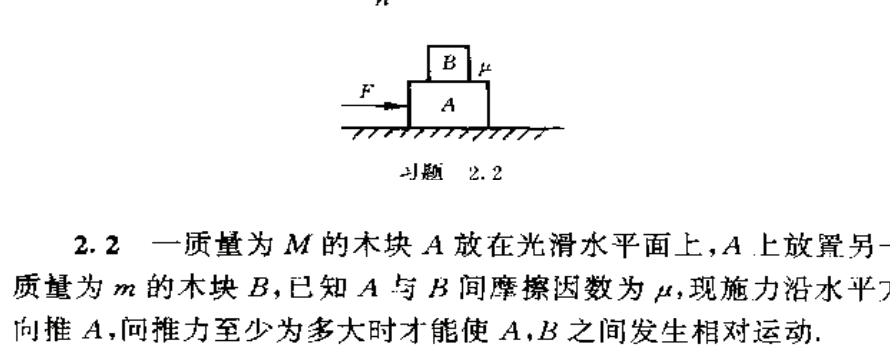
\includegraphics[width=0.72\textwidth]{images/ex-2-2-original.png}
    }{%
        \fbox{\parbox{0.72\textwidth}{\centering 原题图 2.2 预留位置：请将裁切后的图片命名为 \texttt{ex-2-2-original.png} 并放入 \texttt{images/} 目录。}}
    }
    \caption{习题 2.2 原题图}
\end{figure}

设下方木块 $A$ 的质量为 $M$，上方木块 $B$ 的质量为 $m$。水平面光滑，只有 $A$、$B$ 之间存在摩擦，摩擦因数为 $\mu$。若两者不发生相对运动，则它们具有共同加速度
\[
    a=\frac{F}{M+m}.
\]
上方木块 $B$ 的水平方向受力只有静摩擦力，因此所需静摩擦力为
\[
    f_s=ma=\frac{mF}{M+m}.
\]
不发生相对运动要求
\[
    f_s\le \mu mg.
\]
于是
\[
    \frac{mF}{M+m}\le \mu mg.
\]
因此临界推力为
\[
    \boxed{F_{临界}=\mu(M+m)g}.
\]
当 $F$ 大于该值时，所需静摩擦力超过最大静摩擦力，$A$、$B$ 之间发生相对运动。

\begin{center}
\begin{tikzpicture}[scale=1.0,>=stealth]
    \draw[thick] (0,0) rectangle (3.2,0.8);
    \draw[thick] (1.0,0.8) rectangle (2.2,1.5);
    \node at (1.6,0.4) {$A(M)$};
    \node at (1.6,1.15) {$B(m)$};
    \draw[thick] (-0.4,0) -- (3.7,0);
    \draw[->,thick] (-1.0,0.4) -- (0,0.4) node[midway,above] {$F$};
    \draw[->,thick,red] (1.6,1.15) -- (2.5,1.15) node[right] {$f_s$};
    \draw[->,thick,blue] (1.6,0.8) -- (0.7,0.8) node[left] {$f_s'$};
\end{tikzpicture}
\end{center}

本题易错点是把静摩擦力一开始就写成 $\mu mg$。事实上，静摩擦力先由共同运动所需的加速度决定，只有临界状态才达到最大值。

\subsection{例题 2.3：板与物体共同加速及抽板条件}

\begin{figure}[htbp]
    \centering
    \IfFileExists{images/ex-2-3-original.png}{%
        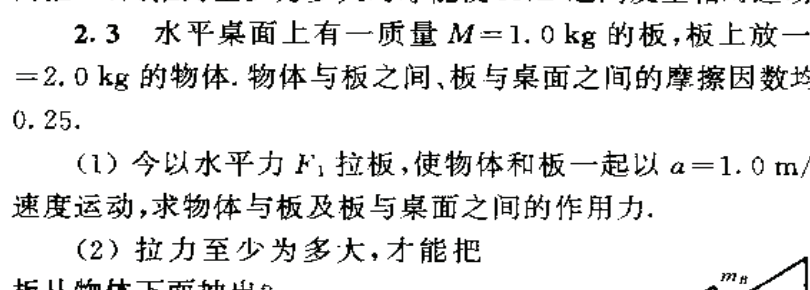
\includegraphics[width=0.82\textwidth]{images/ex-2-3-original.png}
    }{%
        \fbox{\parbox{0.82\textwidth}{\centering 习题 2.3 原题图预留位置：请将裁切后的图片命名为 \texttt{ex-2-3-original.png} 并放入 \texttt{images/} 目录。}}
    }
    \caption{习题 2.3 原题图}
\end{figure}

已知板质量 $M=1.0\,\mathrm{kg}$，物体质量 $m=2.0\,\mathrm{kg}$，物体与板之间、板与桌面之间的摩擦因数均为 $\mu=0.25$。

\subsubsection*{（1）共同以 $a=1.0\,\mathrm{m/s^2}$ 加速}

物体 $m$ 的水平方向受力只有来自板的静摩擦力，因此
\[
    f_1=ma=2.0\times1.0=2.0\,\mathrm{N}.
\]
物体与板之间的正压力为
\[
    N_1=mg=2.0g.
\]
取 $g=9.8\,\mathrm{m/s^2}$，则
\[
    N_1=19.6\,\mathrm{N},\qquad
    f_{1,\max}=\mu N_1=4.9\,\mathrm{N}.
\]
由于所需静摩擦力 $2.0\,\mathrm{N}$ 小于最大静摩擦力，物体与板可保持相对静止。

板与桌面之间的正压力为
\[
    N_2=(M+m)g=3.0g=29.4\,\mathrm{N}.
\]
板相对桌面滑动时，桌面对板的滑动摩擦力大小为
\[
    f_2=\mu N_2=0.25\times29.4=7.35\,\mathrm{N}.
\]
因此，物体与板之间的作用力包括正压力 $19.6\,\mathrm{N}$ 和摩擦力 $2.0\,\mathrm{N}$；板与桌面之间的作用力包括正压力 $29.4\,\mathrm{N}$ 和摩擦力 $7.35\,\mathrm{N}$。

\subsubsection*{（2）刚要把板从物体下抽出}

刚要发生相对滑动时，物体与板之间的静摩擦力达到最大：
\[
    f_{1,\max}=\mu mg.
\]
物体能够随板共同运动的最大加速度为
\[
    a_{\max}=\frac{f_{1,\max}}{m}=\mu g.
\]
把板和物体作为整体，在临界状态下有
\[
    F-\mu(M+m)g=(M+m)a_{\max}.
\]
代入 $a_{\max}=\mu g$，得
\[
    F_{\min}=2\mu(M+m)g.
\]
数值上
\[
    \boxed{F_{\min}=2\times0.25\times3.0\times9.8=14.7\,\mathrm{N}}.
\]

\subsection{例题 2.4：斜面体保持静止的摩擦条件}

\begin{figure}[htbp]
    \centering
    \IfFileExists{images/ex-2-4-original.png}{%
        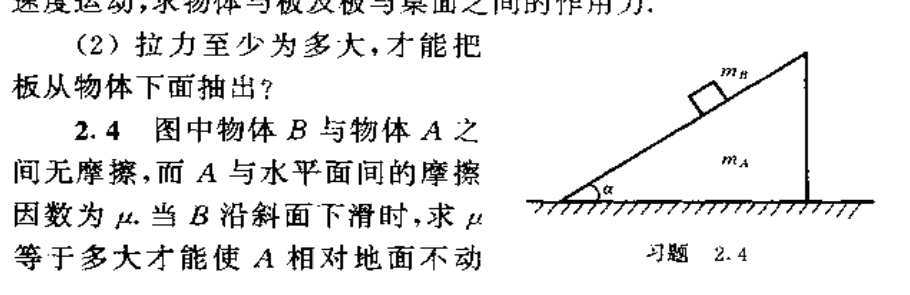
\includegraphics[width=0.82\textwidth]{images/ex-2-4-original.png}
    }{%
        \fbox{\parbox{0.82\textwidth}{\centering 原题图 2.4 预留位置：请将裁切后的图片命名为 \texttt{ex-2-4-original.png} 并放入 \texttt{images/} 目录。}}
    }
    \caption{习题 2.4 原题图}
\end{figure}

物体 $B$ 与斜面体 $A$ 之间无摩擦，$A$ 与水平地面之间的摩擦因数为 $\mu$。设 $B$ 正沿斜面下滑，要求 $A$ 相对地面不动。

由于 $A$ 不动，可把斜面看作固定斜面分析 $B$。垂直斜面方向无加速度，因此
\[
    N=m_Bg\cos\alpha.
\]
这里 $N$ 是斜面 $A$ 对物体 $B$ 的支持力。由牛顿第三定律，$B$ 对 $A$ 的压力大小也为 $N$，方向垂直斜面向右下方。其水平分量为
\[
    N\sin\alpha=m_Bg\sin\alpha\cos\alpha,
\]
竖直向下分量为
\[
    N\cos\alpha=m_Bg\cos^2\alpha.
\]

对斜面体 $A$，地面对它的支持力为
\[
    N_0=m_Ag+N\cos\alpha
       =m_Ag+m_Bg\cos^2\alpha.
\]
为使 $A$ 不动，地面对 $A$ 的静摩擦力必须平衡 $B$ 对 $A$ 的水平推力：
\[
    f_s=N\sin\alpha=m_Bg\sin\alpha\cos\alpha.
\]
静摩擦力不能超过最大静摩擦力：
\[
    f_s\le \mu N_0.
\]
因此
\[
    m_Bg\sin\alpha\cos\alpha
    \le
    \mu\left(m_Ag+m_Bg\cos^2\alpha\right),
\]
化简得
\[
    \boxed{
    \mu \ge
    \frac{m_B\sin\alpha\cos\alpha}
    {m_A+m_B\cos^2\alpha}
    }.
\]

\begin{center}
\begin{tikzpicture}[scale=1.0,>=stealth]
    \coordinate (O) at (0,0);
    \coordinate (R) at (4,0);
    \coordinate (T) at (4,2);
    \draw[thick] (O) -- (R) -- (T) -- cycle;
    \draw[thick] (-0.5,0) -- (4.8,0);
    \node at (2.8,0.7) {$A$};
    \draw[rotate around={26.565:(1.8,1.0)},thick] (1.8,1.0) rectangle (2.35,1.45);
    \node at (2.15,1.35) {$B$};
    \draw[->,thick,red] (4.1,0.8) -- (4.9,0.8) node[right] {$N\sin\alpha$};
    \draw[->,thick,red] (4.1,0.8) -- (4.1,0.1) node[below] {$N\cos\alpha$};
    \draw[->,thick,blue] (1.2,0.15) -- (0.3,0.15) node[left] {$f_s$};
    \draw[->,thick] (2.2,0) arc (0:26.565:2.2);
    \node at (1.0,0.22) {$\alpha$};
\end{tikzpicture}
\end{center}

% !TeX root = ../Fundamental-Physics-B.tex
% 第 2.4 节：绳、滑轮与连接体模型

\section{绳、滑轮与连接体模型}

绳、滑轮和连接体问题的核心是：先明确理想模型条件，再根据约束关系把多个物体的加速度联系起来。若只凭直觉把张力写成 $mg$，或把所有物体的加速度都直接写成相等，往往会导致错误。

\subsection{理想轻绳与理想滑轮}

理想轻绳通常满足以下条件：
\begin{enumerate}
    \item 绳的质量忽略不计；
    \item 绳不可伸长；
    \item 张力方向沿绳；
    \item 同一根轻绳上的张力大小处处相等。
\end{enumerate}

若滑轮也可视为理想滑轮，即滑轮质量和轴摩擦均忽略，则滑轮只改变张力方向，不改变张力大小。因此通过理想定滑轮的同一根轻绳两侧张力大小相等。

\begin{attention}{张力不一定等于重力}{ch2:tension-not-mg}
绳的张力由动力学方程决定。只有物体静止或匀速直线运动且竖直方向只受重力和张力时，才有 $T=mg$。若物体有竖直加速度，一般应写
\[
    T-mg=ma
\]
或按所选正方向列式。
\end{attention}

\subsection{连接体问题中的整体法与隔离法}

连接体问题常用两种方法。

\textbf{整体法}：把多个物体看成一个系统。系统内力在整体方程中相互抵消，适合求系统共同加速度。

\textbf{隔离法}：把其中一个物体单独取出。隔离法适合求物体之间的接触力、绳中张力或某个接触面的摩擦力。

对于轻绳不可伸长的系统，应先写绳长约束，再对时间求导得到速度和加速度关系。最简单的定滑轮模型中，绳两端物体沿绳方向的加速度大小相等、方向相反；动滑轮问题中则不能机械套用“加速度相等”，必须从绳长不变条件出发。

\subsection{例题 2.5：定滑轮拉重物时人对地面的压力}

\begin{figure}[htbp]
    \centering
    \IfFileExists{images/ex-2-5-original.png}{%
        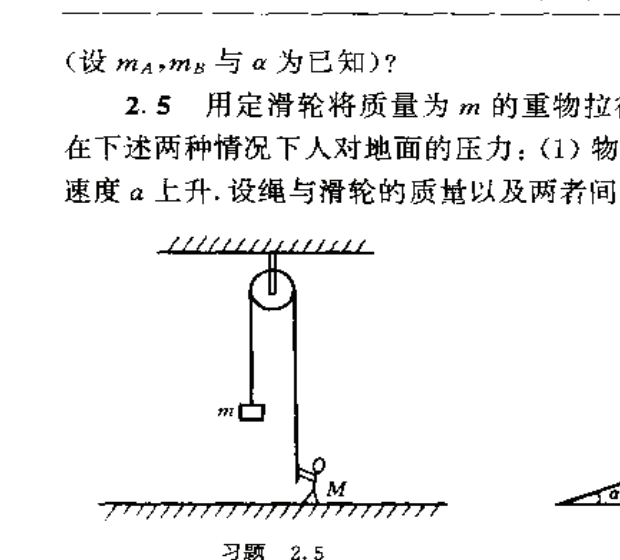
\includegraphics[width=0.62\textwidth]{images/ex-2-5-original.png}
    }{%
        \fbox{\parbox{0.62\textwidth}{\centering 原题图 2.5 预留位置：请将裁切后的图片命名为 \texttt{ex-2-5-original.png} 并放入 \texttt{images/} 目录。}}
    }
    \caption{习题 2.5 原题图}
\end{figure}

定滑轮和绳的质量、摩擦均忽略，因此绳中张力处处相等，记为 $T$。人受三个竖直方向的力：重力 $Mg$ 向下、地面对人的支持力 $N$ 向上、绳对人的拉力 $T$ 向上。人静止在地面上，故
\[
    N+T-Mg=0,
    \qquad
    N=Mg-T.
\]
人对地面的压力大小等于地面对人的支持力大小，即为 $N$。

\subsubsection*{（1）物体匀速上升}

物体匀速上升时加速度为零，对重物有
\[
    T-mg=0,
    \qquad
    T=mg.
\]
因此
\[
    \boxed{N=(M-m)g}.
\]

\subsubsection*{（2）物体以加速度 $a$ 上升}

取竖直向上为正方向。对重物有
\[
    T-mg=ma,
    \qquad
    T=m(g+a).
\]
所以人对地面的压力为
\[
    \boxed{N=Mg-m(g+a)=(M-m)g-ma}.
\]
若该表达式小于等于零，说明人将离开地面，地面对人的支持力不能再按静止接触条件求解。

\begin{center}
\begin{tikzpicture}[scale=1.0,>=stealth]
    \draw[thick] (0,3.0) circle (0.45);
    \draw[thick] (-0.45,3.0) -- (-0.45,1.2);
    \draw[thick] (0.45,3.0) -- (0.45,0.6);
    \draw[thick] (-0.85,3.55) -- (0.85,3.55);
    \draw[thick] (-0.45,1.2) rectangle (-1.05,0.6);
    \node at (-0.75,0.9) {$m$};
    \draw[thick] (0.0,0) -- (1.2,0) -- (1.2,1.4) -- (0.0,1.4) -- cycle;
    \node at (0.6,0.7) {$M$};
    \draw[thick] (-1.3,0) -- (2.0,0);
    \draw[->,thick,red] (0.6,0.7) -- (0.6,1.8) node[above] {$T$};
    \draw[->,thick] (0.6,0.7) -- (0.6,-0.8) node[below] {$Mg$};
    \draw[->,thick,blue] (0.25,0.05) -- (0.25,0.8) node[left] {$N$};
\end{tikzpicture}
\end{center}

\subsection{公式小结}

\begin{knowledge}{常用关系式}{ch2:newton-formula-summary}
\[
\begin{aligned}
&\text{牛顿第二定律：} && \sum \boldsymbol F=m\boldsymbol a,\\
&\text{动量形式：} && \sum \boldsymbol F=\dfrac{\mathrm d\boldsymbol p}{\mathrm dt},\\
&\text{重力：} && G=mg,\\
&\text{胡克定律：} && F=k|\Delta l|,\\
&\text{最大静摩擦力：} && f_{s,\max}=\mu_sN,\\
&\text{滑动摩擦力：} && f_k=\mu_kN,\\
&\text{理想轻绳定滑轮：} && T_1=T_2=T.
\end{aligned}
\]
使用这些公式前，必须先确认研究对象、参考系、接触关系和运动状态。
\end{knowledge}

\section{万有引力定律}
\subsection{万有引力定律的数学形式}
在高中我们就学过万有引力定律了，如果有两个质点，它们的质量分别是$m_1$和$m_2$，它们之间的距离为$r$，那么它们之间的引力大小为
\[
F = G \frac{m_1 m_2}{r^2}
\]
这样的式子是一个标量式，如果想研究复杂的问题，矢量的形式可以免去几何问题，更加容易。我们用$\mathbf{F}_{12}$来表示$m_1$对$m_2$的引力，用$\hat{\mathbf{r}}_{12}$来表示由$m_1$指向$m_2$的单位矢量，由于引力是吸引力，所以方向与$\hat{\mathbf{r}}_{12}$相反。所以万有引力定律为
\[
\mathbf{F}_{12} = -G \frac{m_1 m_2}{r^2} \hat{\mathbf{r}}_{12}
\]
或利用$\hat{\mathbf{r}}_{12}= \mathbf{r}_{12}/r$，上面的式子可以写成
\[
\mathbf{F}_{12} = -G \frac{m_1 m_2}{r^3} \mathbf{r}_{12}
\]
这个式子是一种更常见的形式。

我们接下来将展示矢量形式的好处。
\subsection{质点组对质点的引力}
设空间中有 $N$ 个质点，第 $i$ 个质点的质量为 $m_i$，位置矢量为 $\mathbf{r}_i$。另有一质量为 $M$ 的质点位于 $\mathbf{r}$ 处。接下来我们尝试利用前面的定律求这 $N$ 个质点对 $M$ 的万有引力的合力。

先计算单个质点 $m_i$ 对 $M$ 的引力。令 $\mathbf{R}_{i} = \mathbf{r} - \mathbf{r}_i$ 为从 $m_i$ 指向 $M$ 的位矢，则引力大小为 $G \frac{m_i M}{|\mathbf{R}_{i}|^2}$，方向沿 $\hat{\mathbf{R}}_i = \mathbf{R}_i / |\mathbf{R}_i|$。故
\[
\mathbf{F}_i = -G \frac{m_i M}{|\mathbf{R}_i|^3} \mathbf{R}_i.
\]
所有质点对 $M$ 的总引力为各 $\mathbf{F}_i$ 的矢量和：
\[
\mathbf{F} = \sum_{i=1}^{N} \mathbf{F}_i = G M \sum_{i=1}^{N} m_i \frac{\mathbf{r}_i - \mathbf{r}}{|\mathbf{r} - \mathbf{r}_i|^3}.
\]
假如我们坚持用标量式，恐怕难以应对如此多的质点。

如果我们想研究一个在空间中质量连续分布的物体，那么就无法使用上面的结果了。但是在微积分里，我们通常可以把一个连续的东西，如计算函数曲线与坐标轴围成的面积，拆成若干可以计算的、离散的微元求和。

我们可以把一个连续的物体分割成无数个极小的质量微元 $\mathrm{d}m$，每个微元的尺度趋于零，从而可以视为一个质点，位于 $\mathbf{r}'$ 处。该微元对 $M$ 的引力为
\[
\mathrm{d}\mathbf{F} = -G M \, \mathrm{d}m \, \frac{\mathbf{r} - \mathbf{r}'}{|\mathbf{r} - \mathbf{r}'|^3}.
\]
引入质量密度 $\rho(\mathbf{r}')$，则 $\mathrm{d}m = \rho(\mathbf{r}') \, \mathrm{d}V'$，将所有微元的贡献叠加（即积分），便得到整个连续体对 $M$ 的总引力
\[
\mathbf{F} = -G M \iiint_V \rho(\mathbf{r}') \frac{\mathbf{r} - \mathbf{r}'}{|\mathbf{r} - \mathbf{r}'|^3} \, \mathrm{d}V'.
\]
\subsection{万有引力的性质}
万有引力的方向和大小赋予了其极其独特的性质。
\subsubsection{有心力}
若力 $\mathbf{F}$ 的方向始终通过一个固定点（称为力心），且大小仅依赖于质点至力心的距离 $r$，即 $\mathbf{F} = F(r) \hat{\mathbf{r}}$，则称 $\mathbf{F}$ 为有心力。万有引力就是一种有心力，$m_1$和$m_2$受到的引力始终指向两者的质心，也仅和两者之间的距离有关。

有心力具有许多共有的性质，包括运动将在一个固定的平面内（开普勒第一定律）、角动量守恒（开普勒第二定律）、具有对应的势能（引力势能）等。我们这里不做过多展开，如果对能量比较了解，可以试着求一下引力势能。
\subsubsection{对称球体的引力}
引力的平方反比的特性也赋予了它很独特的魅力。正如我们高中学到的库仑力一样，引力和库仑力是平方反比力。平方反比律导致球对称的球壳内部任意一点的物体将不受这个球壳的引力，对称球或球壳外部的质点受到的引力\textbf{等效于集中质量于球心处的质点对于它的引力}。在静电场中也有类似性质。这一性质的证明比较复杂，可以参考电磁学的教材来类比。

例如我们将地球视为均匀球体，质量为$M$，距离地球$r$处质量为m的卫星受到地球的引力大小为
\[
F = G \frac{Mm}{r^2}
\]
这个结论可以通过三重积分得到，也可以利用上面的性质得到。
\subsection{引力质量与惯性质量}
一个物体可能具有多种与相互作用有关的性质，比如它的电荷量决定了它受到的库仑相互作用的大小、\textbf{引力质量}决定了它受到引力的大小、\textbf{惯性质量}决定了它的惯性的大小。有趣的是，人们利用实验发现，引力质量等于惯性质量，这说明与库仑力和电荷量不同，引力和引力质量似乎更特殊一些。

如果引力质量严格等于惯性质量，那么一个物体在引力场中的牛顿第二定律就可以写为
\[
m \mathbf{a} = -G \frac{M m}{r^2} \hat{\mathbf{r}}
\]
左侧和右侧的$m$分别是惯性质量和引力质量。两边消去$m$，则方程可以简化为
\[
\mathbf{a} = -G \frac{M}{r^2} \hat{\mathbf{r}}
\]
这个微分方程的解将会和质量不再相关，物体在引力场中的运动与其质量无关。
\subsection{万有引力定律的应用}
\subsubsection{重力加速度}
在一个质量为$M$的质点周围，与新放入的研究对象的质量$m$无关的加速度为
\[
\mathbf{a} = -G \frac{M}{r^2} \hat{\mathbf{r}}
\]
只需要用$m$乘上这个加速度，我们就能很容易地获得该物体所受的力。这个加速度是一个关于空间坐标的矢量函数（即矢量场）。

如果忽略地球自转，并认为地球是一个半径为$R$的球体，我们来计算地球表面附近这个加速度的大小。

首先我们先假设有一个质量为$m$的物体作为研究对象，它处于地球表面附近，那么根据前面我们提到的性质，我们可以把地球视为一个质量集中于地心的质点。这样我们可以很容易地求出我们的研究对象所受的力的大小
\[
F = G \frac{Mm}{r^2}
\]
把这个力的大小除以我们研究对象的质量，就能得到物体在地球表面附近的加速度，即重力加速度，大小为
\[
g =\frac{F}{m}= G \frac{M}{R^2}
\]

值得注意的是，上面的讨论仅限于忽略地球自转并把地球当作球体的情况，而实际情况要复杂得多。在实际情况下，需要考虑惯性离心力和科里奥利力等，重力和引力之间存在微小的差异。
\subsubsection{第一宇宙速度}
已知地球质量为M，半径为R，我们来求解在地球表面附近绕地球做圆周运动的卫星的速度$v$。

此问题我们在高中就已经学过了，但我们可以重新审视这个问题。设卫星质量为$m$，在自然坐标系中$\mathbf e_n$指向地心，牛顿第二定律为
\[
m \mathbf a = G \frac{Mm}{R^2} \mathbf e_n
\]
写成分量的形式
\[
a_\tau = 0
\]
\[
a_n =G \frac{M}{R^2}
\]
再利用自然坐标系的结论
\[
a_n = \frac{v^2}{R}
\]
联立即可得到和高中阶段一致的结论
\[
v = \sqrt{\frac{GM}{R}}
\]
\subsubsection{一道经典的问题（选读）}
\noindent \textbf{例：}设地球是一个密度均匀的球体，其密度为$\rho$，重力加速度为$g$。A地正下方有一个半径为$a$的球形空洞，球心O距离地面的距离为$h$（$a<h$），求该地重力加速度$g'$。

\noindent \textbf{分析：}这个问题要求解的是一个完整球体挖去一个球体后剩余部分对于A点处质量为$m$的物体的引力$F'$，随后求出$g' = F'/m$，实际上可以存在两种不同的理解方式。

一种思路是，认为完整地球对于A的引力$mg$来源于两部分，一部分是挖去一部分的球体对A的引力$mg'$，另一部分是被挖去的球体对A的引力$m\Delta g$，而$mg$和$m\Delta g$因为是球体的引力所以特别好求解。做差即可求出$g'$。

另一种思路比较有趣，我们认为实际上被挖去一部分的球体是密度为 $\rho$ 的完整地球和密度为$-\rho$的小球体组合而成的。求出两者的引力求和即可。

\noindent \textbf{解：}以竖直向上为正方向。对于质量为 $m$ 的质点位于地面 A 点，完整地球对它的引力为  
\[
F_0 = -mg
\]  
空洞体积为 $\frac{4}{3}\pi a^3$，缺失的质量为  
\[
m_{\text{hole}} = \rho \cdot \frac{4}{3}\pi a^3.
\]  
地面点到空洞球心的距离为 $h$，故空洞区域原本的物质对质点的引力为  
\[
F_{\text{hole}} = -G \frac{m_{\text{hole}} \, m}{h^2} =- G \frac{\rho \cdot \frac{4}{3}\pi a^3 \, m}{h^2}.
\]  
实际引力为完整地球引力减去空洞部分引力 
\[
F' = F_0 - F_{\text{hole}} = - mg + G \frac{4\pi \rho a^3 m}{3h^2}.
\]  
同时
\[
F' = -mg'
\]
因此该点的重力加速度为  
\[
g' = - \frac{F'}{m} = g - G \frac{4\pi \rho a^3}{3h^2}.
\]  
此即所求重力加速度的表达式。
\section{力学相对性原理与伽利略变换}
\subsection{参考系与坐标系}
\textbf{参考系}是描述物体运动时被选作参照的物体或物体系，它决定了运动的观测结果。
\textbf{坐标系}是固定在参考系上的数学工具，用于定量描述位置和方向。
同一参考系可采用不同的坐标系.参考系是物理的，而坐标系是数学的。

例如，当我们坐在行驶的汽车上观察路边的树时，我们以汽车为参考系，就会看到树以速度$\mathbf v$向我们的后方移动，无论采取何种坐标系，都不能改变树木向我们的后面移动的这种现象。但是，我们可以采用不同的坐标系来描述这个速度矢量$\mathbf v$，如在正方向向前的一维坐标系内，则$\mathbf v = - v \mathbf i$，这里的$\mathbf i$为向前方的单位向量；当然也可以用正方向向后的一维坐标系，那么$\mathbf v = v \mathbf i '$，这里的$\mathbf{ i } '$为向后方的单位向量。我们通过取不同的坐标系就可以让同样的矢量具备不同的分量。

不过坐标系可以很好地帮助我们传递信息。例如我们描述某人正在以速度$v$向西运动，就依靠了东南西北上下这样一个坐标系，这比起一个不依赖于坐标系的矢量$\mathbf v$更具有现实意义。

总结来说，参考系和坐标系是截然不同的两个概念，需要我们严格辨析。我们许多的物理定律是可以不依赖于坐标系的，想要准确描述其规律却可能需要在一个坐标系中才能比较清晰。
\subsection{伽利略变换}
点P在空间中运动，我们尝试在两个惯性系$K$和$K'$中考察其运动。设惯性系 \( K' \) 相对惯性系 \( K \) 以恒定速度 \( u \) 运动，两参考系原点分别为$O'$和$O$。\( P \) 点在 \( K \) 系中的位矢是 \( \mathbf{r} \)，在 \( K' \) 系中的位矢是 \( \mathbf{r}' \)。为简单起见，假定 \( t = 0 \) 时刻两参考系原点重合，则 \( \overrightarrow{OO'} = \mathbf{u} t \)，从而得到如下关系式

\[
\begin{cases} 
\mathbf{r} = \mathbf{r}' + \mathbf{u} t, \\ 
\mathbf{v} = \mathbf{v}' + \mathbf{u}, \\ 
\mathbf{a} = \mathbf{a}'.
\end{cases}
\]
这一式子的形式不依赖于坐标轴的选取。

如果我们再分别在两个参考系中选取两个空间直角坐标系，两者的原点分别固定于$K$和$K'$，$x$轴正方向与$\mathbf u$平行，$y$与$y'$、$z$与$z'$平行，那么上面的变换关系就可以写为如下坐标变换
\[\begin{cases} 
x = x' + ut, \\ 
y = y', \\ 
z = z', \\ 
t = t'. 
\end{cases}\]
这组变换被称为\textbf{伽利略变换}。
\subsection{力学相对性原理}
在经典力学中，如果两个参考系之间没有相对的加速度，且已知其中之一为惯性系，那么另一个也必然是惯性系。这两个惯性系之间是完全对称的，没有谁优谁劣的差异。伽利略提出的\textbf{力学相对性原理}，表述为
\begin{center}
力学规律对一切惯性系等价
\end{center}

我们可以这么理解这一原理。由于我们考虑的两个参考系均为惯性系，彼此之间相对速度恒定，根据上面的伽利略变换，一个物体在两个参考系中的加速度将会一致。这样，如果要求牛顿第二定律$F=ma$成立，两参考系内必然同时具有完全相同的力学规律。

这一原理在数学逻辑上是完全自洽的，但是如果我们直接把该原理表述为“物理规律对一切惯性系等价”，就会在电磁学领域出现一定问题。为了能够涵盖电磁学，保持物理规律的简洁性，我们不能改动动力学规律，所以我们不得不修改我们对于坐标与时间的认识，认为满足相对性原理的坐标变换为洛伦兹变换而非伽利略变换，这就是\textbf{绝对时空观}和\textbf{相对论时空观}的差异。
\section{碰撞}
\begin{definition}[碰撞]
	两个或多个物体相互接近或发生接触时，在极短时间内，物体的运动状态发生显著变化。\
\end{definition}
除了球的撞击、打桩等以外，分子、原子等微观粒子之间的相互作用也是碰撞过程，被称为“散射”

\begin{definition}[正碰]
	对于两球，如果在碰撞前的速度在两球的中心线上，那么碰撞后的速度也都在这一连线上\
\end{definition}
在正碰过程中，由动量守恒定律可以得到$$
m_1v_{10}+m_2v_{20}=m_1v_1+m_2v_2   (1)
$$
\subsection{恢复系数}
碰撞定律：碰撞后两球的分离速度（$v_2-v_1$）与碰撞前的接近速度（$v_{10}-v_{20}$）成正比,
而这一比值由两球的材料性质决定，即：
$$
e=\dfrac{v_2-v_1}{v_{10}-v_{20}}   (2)
$$
通常把e叫做恢复系数
依据不同的e的取值，我们把正碰分为三种情况：
\begin{itemize}
    \item $e=0$:完全非弹性碰撞
    \item $0<e<1$:非弹性碰撞
    \item $e=1$:完全弹性碰撞
    
\end{itemize}
由（1）和（2）式联立可得：
$$
v_1=v_{10}-\dfrac{(1+e)m_2(v_{10}-v_{20})}{m_1+m_2}
$$
$$
v_2=v_{20}+\dfrac{(1+e)m_1(v_{10}-v_{20})}{m_1+m_2}
$$
\subsection{完全弹性碰撞}
令e=1可以得到
$$
v_1=\dfrac{(m_1-m_2)v_{10}+2m_2v_{20}}{m_1+m_2}
$$
$$
v_2=\dfrac{(m_2-m_1)v_{20}+2m_1v_{10}}{m_1+m_2}
$$
\begin{itemize}
    \item 设两球质量相等,即$m_1=m_2$,代入上式可得$v_1=v_{20} v_2=v_{10}$,此时两球的速度和能量发生了转换.

    \item 设$v_{20}=0$可得$v_1=\dfrac{(m_1-m_2)v_{10}}{m_1+m_2} , v_2=\dfrac{2m_1v_{10}}{m_1+m_2}$
    \item 假设$m_2>>m_1$,此时有$v_1=-v_{10},v_2=0$
\end{itemize}
\subsection{完全非弹性碰撞}
由完全非弹性碰撞e=0可得
$$
v_1=v_2=\dfrac{m_1v_{10}+m_2v_{20}}{m_1+m_2}
$$
此时碰撞中损失的机械能到达最大值，为：
$$
\Delta E=\dfrac{1}{2}(1-e^2)\dfrac{m_1m_2}{m_1+m_2}(v_{10}-v_{20})^2
$$
若此时两个物体中有一个物体是静止的（$v_{20}=0$）,则有：
$$
\Delta E=\dfrac{1}{2}(1-e^2)\dfrac{m_1m_2}{m_1+m_2}v_{10}^2
$$

\chapter{动量与冲量}

\section{导言}
在第二章中，我们把力定义为物体间的一种相互作用，通过定义、实验等方式得到了力与加速度的关系，并引入了惯性质量，最终得到牛顿第二定律。作为本章引言，我们暂时忘记第二章的结论，换一种思考方式去审视“力”。

考虑两个除运动状态外完全相同的质点。这两个质点只受到它们之间的相互作用。容易想象，任意时刻 $t$，存在这样一个参考系，在此参考系下，两质点的速度等大反向，即：
\[ \boldsymbol{v}_1 = -\boldsymbol{v}_2 \]
取两质点中点 $O$。根据空间反演对称性，我们断言，在相互作用的 $\Delta t$ 内，两质点的速度增量也是等值反向的：
\[ \Delta \boldsymbol{v}_1 = -\Delta \boldsymbol{v}_2 \]
取 $\Delta t \to 0$ 的极限，得：
\[ \frac{d\boldsymbol{v}_2}{dt} = -\frac{d\boldsymbol{v}_1}{dt} \]
推广至一般质点，考虑到不同质点之间的差异只能由质量（一个标量）表征，将上式改写为：
\[ m_2 \Delta \boldsymbol{v}_2 = -m_1 \Delta \boldsymbol{v}_1 \]
同样取 $\Delta t \to 0$ 的极限，得：
\[ m_2 \frac{d\boldsymbol{v}_2}{dt} = -m_1 \frac{d\boldsymbol{v}_1}{dt} \]
这揭示了一个深刻的物理事实：两个质点在相互作用时，正在相互传递着一个量。并且我们还得出，质点 1 损失多少这个量，质点 2 就得到多少这个量。

最后，我们定义：力是单位时间这个量的传递，即
\[ \text{质点 1 给质点 2 的力：} \quad \boldsymbol{f}_{12} = m_2 \frac{d\boldsymbol{v}_2}{dt} \]
\[ \text{质点 2 给质点 1 的力：} \quad \boldsymbol{f}_{21} = m_1 \frac{d\boldsymbol{v}_1}{dt} \]
代入上述公式得到：
\[ \boldsymbol{f}_{12} + \boldsymbol{f}_{21} = \boldsymbol{0} \]
我们得到了牛顿第三定律。

\begin{knowledge}{力的本质}{ch3:pre-newton-core}
	本节旨在帮助读者理解重要概念：力是动量的传递。
\end{knowledge}

\newpage

\section{冲量与动量定理}
\textit{注：本节我们主要考虑质点的动量，及作用在质点上力的冲量。}

\vspace{1em}
\noindent 对于每个质点，定义其动量为质量与速度的乘积，即：
\[ \boldsymbol{p} = m\boldsymbol{v} \]
\noindent 由导言的分析，或由牛顿第二定律的微分形式，可得：
\[ \boxed{\boldsymbol{F} = \frac{d\boldsymbol{p}}{dt}} \]

\begin{knowledge}{关于牛顿第二定律的思考}{ch3:second-law-essence}
	注意：$\boldsymbol{F} = d\boldsymbol{p}/dt$ 才是牛顿第二定律的更本质形式。事实上，我们无法直接通过 $\boldsymbol{F}=m\boldsymbol{a}$ 得到 $\boldsymbol{F}=d\boldsymbol{p}/dt$，因为这种推导只在 $m$ 为定值时才成立。要注意到：在 $\boldsymbol{F}=d\boldsymbol{p}/dt$ 中，质点的质量是可能变化的。
\end{knowledge}

\noindent 对 $\boxed{\boldsymbol{F} = d\boldsymbol{p}/dt}$ 进行变形：
\[ \boldsymbol{F}dt = d\boldsymbol{p} \]
两边积分：
\[ \int_{t_1}^{t_2} \boldsymbol{F} dt = \boldsymbol{p}_2 - \boldsymbol{p}_1 \]

\noindent 定义冲量 [$\boldsymbol{I} = \int_{t_1}^{t_2} \boldsymbol{F} dt$]。

\noindent 可以看出，冲量是力对时间的累积量，同时冲量也是矢量。利用冲量定义，我们得出动量定理：
\[ \boxed{\boldsymbol{I} = \boldsymbol{p}_2 - \boldsymbol{p}_1 = \Delta \boldsymbol{p}} \]
由于上述公式均为矢量式，我们也可以写成分量形式：
\[ I_x = \Delta p_x, \quad I_y = \Delta p_y, \quad I_z = \Delta p_z \]

\begin{knowledge}{平均力的计算}{ch3:average-force}
	我们可以通过动量定理算出平均力，即 $\bar{\boldsymbol{F}} = \frac{\Delta \boldsymbol{p}}{\Delta t}$。
\end{knowledge}

\subsection*{常见误区}
\begin{enumerate}
	\item \textbf{忽视矢量性：} 在处理反弹、斜碰等问题时，未建立坐标系进行矢量分解，直接做标量加减导致方向错误。
	\item \textbf{混淆变化量概念：} \\
	      动量变化量的大小：$|\boldsymbol{\Delta p}| = |\boldsymbol{p}_2 - \boldsymbol{p}_1|$（矢量差的模）；\\
	      动量大小的变化量：$\Delta|\boldsymbol{p}|  = |\boldsymbol{p}_2| - |\boldsymbol{p}_1|$（标量差）。二者通常不相等。
\end{enumerate}

\vspace{1em}
\noindent\textbf{例题 3.2：} 喷泉中的水柱把一重为 $W$ 的桶顶在空中。已知水以恒定速率 $v_0$、恒定质量增率（单位时间喷出的质量）$Q$ 从地下射向空中，并假设水与桶撞击后以原速率、相反方向反弹，求桶可稳定停留的高度。

\noindent\textbf{解答：}
设桶可稳定停留的高度为 $h$，水柱到达此高度时与桶撞击前的速率为 $v$。根据竖直上抛运动规律，有：
\[ v = \sqrt{v_0^2 - 2gh} \]
在 $\Delta t$ 时间内，撞击桶的水质量为 $\Delta m = Q \Delta t$。规定竖直向上为正方向，对这部分水列动量定理：
\[ F_{\text{水}} \Delta t = \Delta p = \Delta m (-v) - \Delta m v = -2v \Delta m \]
得到桶对水的作用力 $F_{\text{水}}$ 为：
\[ F_{\text{水}} = -2v \frac{\Delta m}{\Delta t} = -2vQ \]
考虑到作用力等于反作用力，水对桶的冲击力 $F$ 大小为 $F = 2vQ$，方向竖直向上。
当桶稳定时受力平衡，令 $F = W$，得到：
\[ 2Q\sqrt{v_0^2 - 2gh} = W \]
两边平方并解得桶可稳定停留的高度 $h$ 为：
\[ h = \frac{v_0^2}{2g} - \frac{W^2}{8gQ^2} \]

\newpage

\section{质点组动量变化定理}
\noindent 对系统每一个质点 $i$，有：
\[ \boldsymbol{F}_{\text{外},i} + \boldsymbol{F}_{\text{内},i} = \frac{d\boldsymbol{p}_i}{dt} \]
\\其中，$\boldsymbol{F}_{\text{外},i}$ 表示第 $i$ 个质点受到的合外力，$\boldsymbol{F}_{\text{内},i}$ 表示第 $i$ 个质点受到的合内力。
\\
\noindent 由牛顿第三定律，内力之和恒为零：
\[ \sum \boldsymbol{F}_{\text{内},i} = \boldsymbol{0} \]
于是得到：
\[ \boxed{\sum \boldsymbol{F}_{\text{外},i} = \frac{d\boldsymbol{P}}{dt}} \]
其中 $\boldsymbol{P} = \sum \boldsymbol{p}_i$，为质点组总动量。

由上面的推导，我们能够得出质点系的一些性质：
\begin{enumerate}
	\item 质点系内力冲量为 0，内力不能改变质点组的总动量。即便是系统内部剧烈的内力交互（如内爆、摩擦），也不会改变系统总动量。
	\item 只有外力才可能改变质点组动量。
\end{enumerate}

\noindent\textbf{例题 3.3：} 质量分别为 $m_1$、$m_2$ 和 $m_3$ 的三个质点 A、B 和 C 位于光滑的水平桌面上，用已拉直的不可伸长的柔软轻绳 AB 和 BC 连接，$\angle ABC = \pi - \alpha$。今有一冲量为 $I$ 的冲击力沿 BC 方向作用于质点 C，求质点 A 开始运动时的速度。

\noindent\textbf{解答：}
设冲击后 A, B, C 速度大小分别为 $v_A, v_B, v_C$。
对 ABC 系统，根据质点组动量定理，在沿 BC 方向与垂直 BC 方向分别列式：

\vspace{1em}
\begin{center}
	\begin{tikzpicture}[>=latex, thick]
		\coordinate (A) at (0, 0);
		\coordinate (B) at (3, 0);
		\coordinate (C) at ($(B) + (30:2.5)$);
		\draw (A) -- (B);
		\draw (B) -- (C);
		\draw[dashed] (B) -- ++(2, 0);
		\draw[->] (B) -- ($(B) + (55:2.5)$) node[left] {$v_B$};
		\draw[->] (C) -- ($(C) + (30:1.5)$) node[right] {$I$};
		\draw ($(B) + (1, 0)$) arc (0:30:1);
		\node at ($(B) + (15:1.25)$) {$\alpha$};
		\draw ($(B) + (30:1.2)$) arc (30:55:1.2);
		\node at ($(B) + (42.5:1.45)$) {$\theta$};
		\filldraw[fill=white, draw=black] (A) circle (2pt) node[below=4pt] {$A$} node[above=4pt] {$m_1$};
		\filldraw[fill=white, draw=black] (B) circle (2pt) node[below=4pt] {$B$} node[above left=4pt and 2pt] {$m_2$};
		\filldraw[fill=white, draw=black] (C) circle (2pt) node[below right=2pt] {$C$} node[above left=2pt] {$m_3$};
	\end{tikzpicture}
\end{center}
\vspace{1em}

\begin{align*}
	\text{沿 BC 方向：} \quad  & I = m_1 v_A \cos\alpha + m_2 v_B \cos\theta + m_3 v_C \\
	\text{垂直 BC 方向：} \quad & 0 = -m_1 v_A \sin\alpha + m_2 v_B \sin\theta
\end{align*}
考虑到绳子不可伸长的约束条件：
\begin{align*}
	\text{沿 AB 绳方向：} \quad & v_A = v_B \cos(\alpha + \theta) \\
	\text{沿 BC 绳方向：} \quad & v_C = v_B \cos\theta
\end{align*}
由上述四式联立。先将速度约束代入动量方程中消去 $v_C$ 和 $\theta$，经过代数化简可解得质点 A 的速度：
\[ v_A = \frac{I m_2 \cos\alpha}{m_2(m_1 + m_2 + m_3) + m_1 m_3 \sin^2\alpha} \]
\textit{注：本题也可以不用质点组动量定理分析，感兴趣的读者可自行研究其他解法。}

\newpage

\section{动量守恒定律}
\noindent 对于一个质点组，无论其内力如何作用，只要合外力为 0，就能保证：
\[ \frac{d\boldsymbol{P}}{dt} = \boldsymbol{0} \]
其中 $\boldsymbol{P}$ 是质点组总动量。

\noindent 这说明，$\boldsymbol{P}$ 不随时间变化，即 $\boldsymbol{P}$ 必定为一个不变的常矢量。

\noindent\textbf{说明：}
\begin{enumerate}
	\item 由动量定理的分量式，若质点组在某一方向（以 $x$ 方向为例）合力为零，仍然有 $P_x = \text{常数}$。
	\item 动量守恒定律是一个极其普适的定律。无论是低速宏观物体的碰撞，还是高速微观粒子的裂变，动量守恒均成立。
	\item 若满足以下特殊情况，可认为质点组总动量近似守恒：
	      \begin{itemize}
		      \item 外力的大小远小于内力，如外力有上限（如滑动摩擦力），而内力极大（如二体碰撞时的冲击力）。
		      \item 外力有限且作用时间 $\Delta t \to 0$。例如包含重力或摩擦力的问题。此时由于 $\Delta t \to 0$，冲量 $F_{\text{外}}\Delta t \to 0$，故可认为系统动量近似守恒。
	      \end{itemize}
\end{enumerate}

\section{火箭喷气与变质量问题}

火箭喷气问题属于变质量系统动力学问题。普通形式
\[
    \sum \boldsymbol F=m\boldsymbol a
\]
默认研究对象质量不变；而火箭在喷气过程中不断抛出燃料，主体质量随时间减小。如果仍把火箭看作恒质量质点，便会漏掉喷出质量携带的动量流。

\subsection{变质量系统的动量分析}

设某时刻火箭主体质量为 $m$，相对地面惯性系的速度为 $\boldsymbol v$。在极短时间 $\mathrm dt$ 内，火箭喷出一小部分燃料，主体质量变为
\[
    m+\mathrm dm ,
\]
其中喷气时火箭主体质量减少，所以
\[
    \mathrm dm<0.
\]
喷出燃料相对火箭主体的速度记为 $\boldsymbol u$。注意，$\boldsymbol u$ 是喷出物相对火箭的速度，不是喷出物相对地面的速度。

取“火箭主体 + 即将喷出的燃料”为研究系统，由质点组动量变化定理可知
\[
    \boldsymbol I_{\mathrm{ext}}=\Delta \boldsymbol P .
\]
在 $\mathrm dt$ 很小时，外力冲量为 $\boldsymbol F_{\mathrm{ext}}\mathrm dt$。保留一阶小量，可得变质量运动方程
\[
    \boxed{
    m\frac{\mathrm d\boldsymbol v}{\mathrm dt}
    =
    \boldsymbol F_{\mathrm{ext}}
    +
    \boldsymbol u\frac{\mathrm dm}{\mathrm dt}
    } .
\]
式中 $\boldsymbol F_{\mathrm{ext}}$ 为火箭主体所受外力，如重力、空气阻力等。若喷气方向与火箭前进方向相反，则 $\boldsymbol u$ 指向火箭后方；又因为 $\mathrm dm/\mathrm dt<0$，喷气项可使火箭获得向前的加速度。

\begin{note}
变质量运动方程中的 $m$ 指火箭主体当前质量，$\mathrm dm$ 指火箭主体质量变化量。喷气时 $\mathrm dm<0$，这是最容易出错的符号约定。
\end{note}

\subsection{无外力一维火箭公式}

若火箭在远离天体引力和空气阻力的空间中沿直线运动，取火箭前进方向为正方向。设喷气相对火箭向后，喷气速度大小为 $v_r$，则
\[
    \boldsymbol u=-v_r\boldsymbol e_x .
\]
无外力时，变质量运动方程化为
\[
    m\frac{\mathrm dv}{\mathrm dt}
    =
    -v_r\frac{\mathrm dm}{\mathrm dt}.
\]
写成微分形式：
\[
    \mathrm dv=-v_r\frac{\mathrm dm}{m}.
\]
若 $v_r$ 近似为常量，从初始质量 $m_0$、初速度 $v_0$ 积分到当前质量 $m$、速度 $v$，有
\[
    \int_{v_0}^{v}\mathrm dv
    =
    -v_r\int_{m_0}^{m}\frac{\mathrm dm}{m}.
\]
因此
\[
    v-v_0
    =
    -v_r\ln\frac{m}{m_0}
    =
    v_r\ln\frac{m_0}{m}.
\]
理想火箭公式为
\[
    \boxed{
    v=v_0+v_r\ln\frac{m_0}{m}
    } .
\]
它说明火箭速度增量与喷气速度 $v_r$ 成正比，并与质量比 $m_0/m$ 的对数成正比。

\subsection{速度参考系的辨析}

火箭问题中至少涉及两类速度：

\begin{enumerate}
    \item $\boldsymbol v$：火箭主体相对地面惯性系的速度；
    \item $\boldsymbol u$：喷出物相对火箭主体的速度；
    \item 喷出物相对地面惯性系的速度约为 $\boldsymbol v+\boldsymbol u$。
\end{enumerate}

列动量方程时，所有动量都必须在同一个惯性系中表达，不能把相对火箭的喷气速度直接当作喷出物对地速度。

\subsection{例题：理想火箭速度}

一枚火箭在无外力空间中沿直线运动。初始质量为 $m_0$，初速度为 $v_0$，喷气相对火箭向后，喷气速度大小恒为 $v_r$。当火箭质量减小到 $m$ 时，求火箭速度。

\textbf{解析：} 取火箭前进方向为正方向。无外力时，
\[
    m\frac{\mathrm dv}{\mathrm dt}
    =
    -v_r\frac{\mathrm dm}{\mathrm dt}.
\]
因为喷气时 $\mathrm dm<0$，所以右端为正，火箭加速。分离变量得
\[
    \mathrm dv=-v_r\frac{\mathrm dm}{m}.
\]
积分：
\[
    v-v_0=-v_r\ln\frac{m}{m_0}.
\]
于是
\[
    \boxed{
    v=v_0+v_r\ln\frac{m_0}{m}
    } .
\]
若 $m$ 越小、$m_0/m$ 越大，火箭速度增量越大；但由于是对数关系，单纯增大质量比的收益会逐渐降低。

\subsection{常用公式}

\[
    \boxed{
    m\frac{\mathrm d\boldsymbol v}{\mathrm dt}
    =
    \boldsymbol F_{\mathrm{ext}}
    +
    \boldsymbol u\frac{\mathrm dm}{\mathrm dt}
    }
\]
\[
    \boxed{
    v=v_0+v_r\ln\frac{m_0}{m}
    }
    \qquad
    \text{无外力、一维运动、喷气速度恒定时成立。}
\]


\chapter{动能与势能}

\section{章节主线与学习目标}

本章研究力的空间累积效应与机械能转化规律。上一章的动量定理强调力对时间的累积：
\[
    \boldsymbol I=\int \boldsymbol F\,\mathrm dt,
\]
而本章的功与能量方法强调力对位移的累积：
\[
    W=\int \boldsymbol F\cdot\mathrm d\boldsymbol r .
\]
二者都来源于牛顿第二定律，但适用对象和物理意义不同。

\subsection{本章主线}

动能与势能一章可以按如下脉络学习：
\[
    \text{功与功率}
    \longrightarrow
    \text{动能定理}
    \longrightarrow
    \text{保守力与势能}
    \longrightarrow
    \text{功能原理}
    \longrightarrow
    \text{机械能守恒定律}.
\]
本节之后将先讨论功与功率，再由牛顿第二定律推出动能定理。保守力、势能、功能原理以及机械能守恒定律将在后续章节中继续展开。

\subsection{学习目标}

学习本章前半部分，应掌握以下内容：

\begin{enumerate}
    \item 理解功的定义
    \[
        W=\int_a^b\boldsymbol F\cdot\mathrm d\boldsymbol r,
    \]
    明确“只有力沿位移方向的分量做功”；
    \item 掌握瞬时功率
    \[
        P=\boldsymbol F\cdot\boldsymbol v,
    \]
    理解功率描述做功快慢，而不是力的大小；
    \item 掌握质点动能定理
    \[
        W_{\mathrm{net}}=\Delta E_k,
    \]
    并能用它处理已知位移、求速率的问题；
    \item 区分动量方法与能量方法：冲量改变动量，功改变动能；
    \item 能根据题目条件选择牛顿第二定律、动量定理或动能定理。
\end{enumerate}

\subsection{动量方法与能量方法的选择}

若题目强调力作用的时间、碰撞过程中的平均力或动量变化，通常优先考虑动量定理：
\[
    \boldsymbol I=\Delta\boldsymbol p.
\]
若题目强调运动路径、位移、速度大小变化或不需要求时间，通常优先考虑功与动能定理：
\[
    W_{\mathrm{net}}=\Delta E_k.
\]
简单地说，出现 $\Delta t$ 时先想到冲量，出现 $\mathrm d\boldsymbol r$ 或路径长度时先想到功。

\newpage

\section{功与功率}

功描述力在空间位移上的累积效应。不能把功简单理解成“力的大小乘以路程”，因为只有力在位移方向上的分量参与做功。功率则描述做功的快慢。

\subsection{恒力做功}

若物体在恒力 $\boldsymbol F$ 作用下发生位移 $\boldsymbol s$，力与位移夹角为 $\theta$，则该力做功为
\[
    W=\boldsymbol F\cdot\boldsymbol s=Fs\cos\theta .
\]
因此：

\begin{enumerate}
    \item 当 $0\leq \theta<90^\circ$ 时，$W>0$，力做正功；
    \item 当 $\theta=90^\circ$ 时，$W=0$，力不做功；
    \item 当 $90^\circ<\theta\leq 180^\circ$ 时，$W<0$，力做负功。
\end{enumerate}

功是标量。功的正负表示能量转移方向，不表示空间方向。

\subsection{变力做功}

若力随位置变化，或物体沿曲线运动，则应把路径分成许多微小位移元 $\mathrm d\boldsymbol r$。在每一小段上，元功为
\[
    \mathrm dW=\boldsymbol F\cdot\mathrm d\boldsymbol r .
\]
从起点 $a$ 到终点 $b$ 的总功为
\[
    \boxed{
    W=\int_a^b\boldsymbol F\cdot\mathrm d\boldsymbol r
    } .
\]
在直角坐标系中可写为
\[
    W=\int_a^b
    \left(
    F_x\,\mathrm dx+F_y\,\mathrm dy+F_z\,\mathrm dz
    \right).
\]
计算变力做功时，应沿实际路径积分，不能随意取始末力的平均值乘总位移。

\subsection{合力做功}

若物体受到多个力
\[
    \boldsymbol F_1,\boldsymbol F_2,\cdots,\boldsymbol F_n,
\]
则合力为
\[
    \boldsymbol F_{\mathrm{net}}=\sum_{i=1}^{n}\boldsymbol F_i .
\]
合力做功为
\[
    W_{\mathrm{net}}
    =
    \int \boldsymbol F_{\mathrm{net}}\cdot\mathrm d\boldsymbol r
    =
    \sum_{i=1}^{n}
    \int \boldsymbol F_i\cdot\mathrm d\boldsymbol r
    =
    \sum_{i=1}^{n}W_i .
\]
所以，合力做功等于各分力做功的代数和。

\subsection{功率}

平均功率定义为
\[
    \bar P=\frac{\Delta W}{\Delta t}.
\]
瞬时功率为
\[
    P=\frac{\mathrm dW}{\mathrm dt}.
\]
由 $\mathrm dW=\boldsymbol F\cdot\mathrm d\boldsymbol r$ 得
\[
    \boxed{
    P=\boldsymbol F\cdot\boldsymbol v
    } .
\]
若力与速度夹角为 $\theta$，则
\[
    P=Fv\cos\theta .
\]
功率单位为瓦特：
\[
    1\,\mathrm W=1\,\mathrm{J/s}.
\]

\subsection{功的相对性}

功与参考系有关。因为位移 $\mathrm d\boldsymbol r$ 和速度 $\boldsymbol v$ 都依赖参考系，所以同一个力在不同惯性系中做功和功率一般不同。与此同时，动能也依赖参考系；只要在同一参考系内计算，功与动能之间仍满足动能定理。

\subsection{例题：变力沿直线做功}

质点沿 $x$ 轴从 $x=0$ 运动到 $x=a$。作用在质点上的力为
\[
    F_x=kx,\qquad F_y=F_z=0,
\]
其中 $k$ 为常量。求该力做的功。

\textbf{解析：} 因为质点沿 $x$ 轴运动，
\[
    \mathrm d\boldsymbol r=\mathrm dx\,\boldsymbol e_x.
\]
元功为
\[
    \mathrm dW=\boldsymbol F\cdot\mathrm d\boldsymbol r=kx\,\mathrm dx.
\]
故
\[
    W=\int_0^a kx\,\mathrm dx=\frac{1}{2}ka^2.
\]
因此
\[
    \boxed{W=\frac{1}{2}ka^2}.
\]
本题体现了变力做功必须积分，不能简单套用恒力做功公式。

\subsection{常用公式}

\[
    W=\boldsymbol F\cdot\boldsymbol s=Fs\cos\theta
\]
\[
    \boxed{
    W=\int_a^b\boldsymbol F\cdot\mathrm d\boldsymbol r
    =
    \int_a^b
    \left(
    F_x\,\mathrm dx+F_y\,\mathrm dy+F_z\,\mathrm dz
    \right)
    }
\]
\[
    \boxed{
    P=\frac{\mathrm dW}{\mathrm dt}=\boldsymbol F\cdot\boldsymbol v
    }
\]

\newpage

\section{动能定理}

动能定理将合外力做功与质点动能变化联系起来。它是牛顿第二定律的能量形式，在处理已知位移、求速率的问题时尤其方便。

\subsection{质点动能}

质点动能定义为
\[
    \boxed{
    E_k=\frac{1}{2}mv^2
    } .
\]
动能是标量，只与速率大小有关，与速度方向无关。由于速度依赖参考系，动能也依赖参考系。

\subsection{动能定理的推导}

对质量恒定的质点 $m$，在惯性参考系中，在合外力 $\boldsymbol F_{\mathrm{net}}$ 作用下运动。由牛顿第二定律
\[
    \boldsymbol F_{\mathrm{net}}=m\boldsymbol a
\]
可得合外力元功
\[
    \mathrm dW_{\mathrm{net}}
    =
    \boldsymbol F_{\mathrm{net}}\cdot\mathrm d\boldsymbol r
    =
    m\boldsymbol a\cdot\mathrm d\boldsymbol r .
\]
又因为
\[
    \boldsymbol a=\frac{\mathrm d\boldsymbol v}{\mathrm dt},
    \qquad
    \mathrm d\boldsymbol r=\boldsymbol v\,\mathrm dt,
\]
所以
\[
    \mathrm dW_{\mathrm{net}}
    =
    m\frac{\mathrm d\boldsymbol v}{\mathrm dt}\cdot\boldsymbol v\,\mathrm dt
    =
    m\boldsymbol v\cdot\mathrm d\boldsymbol v .
\]
由
\[
    \mathrm d(v^2)
    =
    \mathrm d(\boldsymbol v\cdot\boldsymbol v)
    =
    2\boldsymbol v\cdot\mathrm d\boldsymbol v
\]
可得
\[
    m\boldsymbol v\cdot\mathrm d\boldsymbol v
    =
    \mathrm d\left(\frac{1}{2}mv^2\right).
\]
因此
\[
    \mathrm dW_{\mathrm{net}}=\mathrm dE_k.
\]
从初态到末态积分，得到
\[
    \boxed{
    W_{\mathrm{net}}
    =
    \Delta E_k
    =
    \frac{1}{2}mv_2^2-\frac{1}{2}mv_1^2
    } .
\]

\subsection{使用步骤}

应用动能定理时，可按以下顺序处理：

\begin{enumerate}
    \item 选定研究对象；
    \item 明确初态和末态；
    \item 判断哪些力做功，哪些力不做功；
    \item 写出合外力做功 $W_{\mathrm{net}}$；
    \item 写出动能变化 $\Delta E_k$；
    \item 建立方程
    \[
        W_{\mathrm{net}}=\Delta E_k
    \]
    并求解未知量。
\end{enumerate}

动能定理不直接涉及时间，因此当题目只关心经过某段位移后的速度大小时，通常比逐步求加速度和时间更简洁。

\subsection{与动量定理的区别}

动量定理为
\[
    \boldsymbol I=\Delta\boldsymbol p,
\qquad
    \boldsymbol I=\int\boldsymbol F\,\mathrm dt,
\]
它体现力对时间的累积。动能定理为
\[
    W_{\mathrm{net}}=\Delta E_k,
\qquad
    W=\int\boldsymbol F\cdot\mathrm d\boldsymbol r,
\]
它体现力对空间位移的累积。

因此：

\begin{enumerate}
    \item 冲量是矢量，功是标量；
    \item 动量变化由冲量决定，动能变化由合外力做功决定；
    \item 动量定理保留速度方向信息，动能定理主要处理速率大小变化。
\end{enumerate}

\subsection{例题：粗糙水平面上的制动距离}

质量为 $m$ 的物块以初速度 $v_0$ 在粗糙水平面上滑行，动摩擦因数为 $\mu$。求物块停止前滑行距离 $s$。

\textbf{解析：} 物块受到重力、支持力和滑动摩擦力。重力和支持力都垂直于位移，不做功；滑动摩擦力方向与位移方向相反，大小为
\[
    f_k=\mu mg.
\]
摩擦力做功为
\[
    W_f=-f_ks=-\mu mgs.
\]
物块末速度为零，所以
\[
    \Delta E_k=0-\frac{1}{2}mv_0^2.
\]
由动能定理
\[
    -\mu mgs=-\frac{1}{2}mv_0^2.
\]
解得
\[
    \boxed{
    s=\frac{v_0^2}{2\mu g}
    } .
\]

\subsection{例题：斜向拉力做功}

质量为 $m$ 的物块在水平面上运动，受到大小为 $F$、与水平面夹角为 $\theta$ 的拉力作用，水平位移为 $s$。若忽略摩擦，求拉力做功与物块动能变化。

\textbf{解析：} 位移方向水平，拉力沿位移方向的分量为
\[
    F_x=F\cos\theta.
\]
拉力做功为
\[
    W=Fs\cos\theta.
\]
重力和支持力都垂直于水平位移，不做功。由动能定理
\[
    \Delta E_k=W=Fs\cos\theta.
\]
因此
\[
    \boxed{
    \Delta E_k=Fs\cos\theta
    } .
\]
这说明并非整个拉力都改变动能，只有沿位移方向的分量做功。

\subsection{常用公式}

\[
    \boxed{
    E_k=\frac{1}{2}mv^2
    }
\]
\[
    \boxed{
    W_{\mathrm{net}}=\Delta E_k
    =
    \frac{1}{2}mv_2^2-\frac{1}{2}mv_1^2
    }
\]
\[
    \boldsymbol I=\int\boldsymbol F\,\mathrm dt,\qquad
    W=\int\boldsymbol F\cdot\mathrm d\boldsymbol r.
\]


\section{保守力与势能}
\textit{本节理论性比较强，许多内容与数分下册重合，大家可以结合数学教材一并复习。本节中绿色文本框内的内容为物理，蓝色文本框内的内容为数学，大家可以比照着看。如果实在看不懂推理过程，可以对物理部分记忆。}
\subsection{保守力}
\begin{tcolorbox}[colback=white!5!white,colframe=green!50!black,title=保守力的定义]
    \textbf{定义}：如果力对物体所做的\textbf{功与路径无关}，只与物体的起点和终点位置有关，则该力称为\textbf{保守力}。

\end{tcolorbox}
这个定义很难不让人联想到数学中的内容。在数学中，我们已经学习过了许多关于第二类曲线积分和第二类曲面积分的性质，比如下面这个很有意思的性质。不知道大家还是否记得如何证明它们的等价性。
\begin{tcolorbox}[colback=white!5!white, colframe=blue!75!black, title=曲线积分与路径无关的等价条件]
    \textbf{定理}：设 \(\mathbf{F} = P(x,y,z)\,\mathbf{i} + Q(x,y,z)\,\mathbf{j} + R(x,y,z)\,\mathbf{k}\) 是定义在单连通区域 \(\Omega \subseteq \mathbb{R}^3\) 上的连续向量场。则以下四个条件等价：
    \begin{enumerate}
        \item 曲线积分 \(\int_{\Gamma} \mathbf{F}\cdot d\mathbf{r}\) 只与起点和终点有关，与路径 \(\Gamma\) 无关。
        \item 对任意闭合曲线 \(C \subset \Omega\)，有 \(\oint_{C} \mathbf{F}\cdot d\mathbf{r} = 0\)。
        \item 存在一个标量函数 \(V\)，使得 \(\mathbf{F} = \nabla V\)。
        \item \(\nabla \times \mathbf{F} = \mathbf{0}\)，具体可写为
              \[
                  \frac{\partial R}{\partial y} - \frac{\partial Q}{\partial z} = 0,\quad
                  \frac{\partial P}{\partial z} - \frac{\partial R}{\partial x} = 0,\quad
                  \frac{\partial Q}{\partial x} - \frac{\partial P}{\partial y} = 0.
              \]
    \end{enumerate}
\end{tcolorbox}

上面数学定理的证明请参见数学分析教材。
当然，我们可以仿照数学定理给出保守力的等价定义。

\begin{tcolorbox}[colback=white!5!white, colframe=green!50!black, title=保守力的等价定义]
    设力场 \(\mathbf{F}=(F_x,F_y,F_z)\) 连续可微且定义在单连通区域上，则以下等价：
    \begin{enumerate}
        \item 做功与路径无关，即$\mathbf{F}$是保守力；
        \item 对任意闭路 \(C\) 有 \(\oint_C \mathbf{F}\cdot d\mathbf{r}=0\)，即$\mathbf{F}$沿闭合路径做功一周净功为0；
        \item 存在势函数 \(V\) 使 \(\mathbf{F}=-\nabla V\)；
        \item \(\nabla\times\mathbf{F}=0\)，即$\mathbf{F}$是无旋场，可简便记忆行列式形式
              \[\nabla\times\mathbf{F} =
                  \begin{vmatrix}
                      \mathbf{i}                  & \mathbf{j}                  & \mathbf{k}                  \\[2pt]
                      \frac{\partial}{\partial x} & \frac{\partial}{\partial y} & \frac{\partial}{\partial z} \\[2pt]
                      F_x                         & F_y                         & F_z
                  \end{vmatrix} = \mathbf{0}.
              \]
    \end{enumerate}
\end{tcolorbox}

这个定理的证明完全可以利用上面数学上的定理。

\noindent\textbf{注：}行列式可以很容易地表示两个矢量叉乘，将基矢依次置于第一行，第一个矢量和第二个矢量的分量依次置于二三行，行列式就是叉乘的结果，即

\[
    \mathbf{A} \times \mathbf{B} =
    \begin{vmatrix}
        \mathbf{i} & \mathbf{j} & \mathbf{k} \\
        A_x        & A_y        & A_z        \\
        B_x        & B_y        & B_z
    \end{vmatrix}
    = (A_y B_z - A_z B_y)\,\mathbf{i} + (A_z B_x - A_x B_z)\,\mathbf{j} + (A_x B_y - A_y B_x)\,\mathbf{k}
\]

考虑到大家的数学可能没学会，我们这里给出不是很严格的证明，方便大家理解这四者的关系。

\noindent\textbf{证明：}一些公式和技巧在电磁场、流场等内容十分重要，我们尝试结合证明过程给出一些

\noindent（1）先证明1和2等价。这涉及到积分路径的构造，这种技巧在电磁学中十分常见。

我们知道对于任意路径$\Gamma$，沿着路径做的功$ W(\Gamma) = \int_{\Gamma}  \mathbf{F}\cdot d\mathbf{r} $只与起点和终点有关，那么对于我们所选取的任意闭合路径C，我们可以将其拆成$C_1$和$C_2$两部分，即$C = C_1 +C_2$，而$C_2$的反方向$-C_2$是一段与$C_1$同起点和终点的不同路径，因此
\[
    \oint_C \mathbf{F}\cdot d\mathbf{r}=( \int_{C_1} + \int_{C_2} )\mathbf{F}\cdot d\mathbf{r} = ( \int_{C_1} - \int_{- C_2} )\mathbf{F}\cdot d\mathbf{r} = 0
\]
同样，如果我们知道了2，就可以将由点A到点B待比较功大小的两条路径$\Gamma_1$和$\Gamma_2$组成闭合回路$C = \Gamma_1 - \Gamma_2$，便可以证明这两条路径上功相等。

\noindent（2）2和4的等价性是显然的。因为Stokes公式
\[
    \oint_{\partial \Sigma} \mathbf{F} \cdot d\mathbf{r}
    = \iint_{\Sigma} (\nabla \times \mathbf{F}) \cdot \mathbf{n} \, dS
\]
对任意闭合路径左侧积分等于0可以给出$\nabla \times \mathbf{F} = 0$，反之亦然。这一公式在电磁场中依旧重要。

\noindent（3）3和4之间的等价性依旧显然。利用恒等式
\[
    \nabla \times \nabla V = 0
\]
如果矢量满足3，则自动满足4；如果矢量满足4，则它一定是某些标量的梯度（或负梯度），且该标量的选取不唯一，可以相差一个常数。因此，我们通过保守力定义这个函数V时，\textbf{需要规定V的零点}。类似的技巧在电磁场中依旧十分常见。在后面我们将会看到这个V的物理含义。
\hfill$\square$

相信大家已经被数学绕晕了。如果你此时大脑依旧清晰，说明你具备了一定学习理论物理的潜质（\textit{那么欢迎来}19\textit{系}doge）；如果你看不懂，完全不必担心。我们改造一下上面的定理，让它简单一些，作为本节的小节。
\begin{tcolorbox}[colback=white!5!white, colframe=red!75!black, title=保守力小结]
    如果 \(\mathbf{F}\) 做功与路径无关，则定义$\mathbf{F}$是保守力。其具有如下三条性质：
    \begin{enumerate}
        \item 保守力沿闭合路径做功一周净功为0；
        \item 存在势函数 \(V\) 使 \(\mathbf{F}=-\nabla V\)；
        \item 保守力场是无旋场
    \end{enumerate}
    对于某一个力，任意证明其一则可表明其是保守力。
\end{tcolorbox}
%%%%%%%%%%%%%%%%%%%%%%%%%%%%%%%%%%%%%%%%%%%%%%%%%%%%%%%%%%%%
\subsection{保守力场的势能}
我们前面讲到，保守力沿某个路径做的功仅与所选取的始末点有关。假如我们固定终点O，而起点是空间中的任意一点Q，那么我们就构建了一个关于空间的函数，这个函数的直接含义是空间中的某一点到O力做的功，即
\[
    W(\textbf{r}) = \int_{Q(\textbf{r})}^{O}  \mathbf{F}\cdot d\mathbf{r} = -  \int_{O}^{Q(\textbf{r})}  \mathbf{F}\cdot d\mathbf{r}
\]
这是一个变限积分。
如果发生小变动$\Delta x$使得终点移动到Q‘，QQ'是平行于x轴、长为$\Delta x$的线段，用$F_x (x,y,z)$表示$F$的$x$分量，
\[
    \begin{aligned}
        W(x+\Delta x,y,z) - W(x,y,z) & = -  \int_{(x,y,z)}^{(x+\Delta x,y,z)}  \mathbf{F}\cdot d\mathbf{r} \\&= -  F_x (x+\theta \Delta x,y,z) \Delta x
    \end{aligned}
\]
应用中值定理有
\[
    \frac{\partial W}{\partial x} = - F_x
\]
同理可得其余两个方向的偏导数，最终得到：
\[
    \mathbf{F}=-\nabla W
\]
这表明，我们定义的此函数W恰好可以作为我们上节中要找的函数V，且W加减任意常数也可以是我们要找的V。
\begin{tcolorbox}[colback=white!5!white,colframe=green!50!black,title=保守力场势能的定义]
    \textbf{定义}：在保守力场中，定义点$Q(\textbf{r})$处的势能为
    \[
        E_p(\textbf{r}) = \int_{Q(\textbf{r})}^{O}  \mathbf{F}\cdot d\mathbf{r}
    \]
    其中O点为势能零点的位置。
\end{tcolorbox}

我们前面反复提到，势能函数V增减任意常数都能符合保守力应当满足的性质，因为无论我们增加一个多大的常数，其梯度依旧不会改变，这将不会改变保守力的大小和方向。事实上，势能零点的选取只会改变势能的绝对大小，不会改变相对大小关系，所以这不会改变任何力学上的结构。因此势能函数可以加上任意有限常数，这个常数不会改变势能差，也不会改变由 $\mathbf F=-\nabla V$ 得到的力。只要选取的势能零点不是奇异点，那么得到的力学规律都是正确的。

我们可以给出如下性质：
\begin{tcolorbox}[colback=white!5!white,colframe=green!50!black,title=保守力场中的势能差]
    \textbf{性质}：在保守力场中，两点的势能差与所选取的势能零点无关。
\end{tcolorbox}

\noindent \textbf{证明：}我们基于势能零点O计算A和B的势能差
\[
    E_p(A) - E_p(B) = \int_{A}^{O}  \mathbf{F}\cdot d\mathbf{r}  - \int_{B}^{O}  \mathbf{F}\cdot d\mathbf{r} = \int_{A}^{B}  \mathbf{F}\cdot d\mathbf{r}
\]
根据保守力的定义，我们得到最右侧的积分只依赖于起点和终点，所以势能差不依赖于势能零点O的选取方式。\hfill$\square$
\begin{tcolorbox}[colback=white!5!white, colframe=red!75!black, title=保守场势能小结]
    \begin{enumerate}
        \item 点$Q$处的势能为$
                  E_p(\textbf{r}) = \int_{Q(\textbf{r})}^{O}  \mathbf{F}\cdot d\mathbf{r}
              $（\textbf{请务必注意积分的上下限顺序}，避免多出一个负号），
              与选取的势能零点O有关；
        \item 两点间的势能差与势能零点O无关。
    \end{enumerate}
\end{tcolorbox}
%%%%%%%%%%%%%%%%%%%%%%%%%%%%%%%%%%%%%%%%%%%%%%%%%%%%%%%%%%%%%%%%%%%%%
\subsection{保守力的实例}
我们熟知的许多力都是保守力。
\begin{tcolorbox}[colback=white!5!white,colframe=green!50!black,title=重力]
    证明重力是保守力。并给出重力势能的形式。
\end{tcolorbox}
\noindent \textbf{证明：}设三维坐标系的z轴竖直向上，坐标原点O位于地面上，重力$\mathbf{F} = -mg \mathbf{k}$。

\textbf{方法一：}计算重力的旋度：
\[
    \begin{aligned}
        \nabla \times \mathbf{F} & =
        \begin{vmatrix}
            \mathbf{i}                  & \mathbf{j}                  & \mathbf{k}                  \\
            \frac{\partial}{\partial x} & \frac{\partial}{\partial y} & \frac{\partial}{\partial z} \\
            0                           & 0                           & -mg
        \end{vmatrix}
        \\&= \mathbf{i}\left(\frac{\partial (-mg)}{\partial y} - \frac{\partial 0}{\partial z}\right) - \mathbf{j}\left(\frac{\partial (-mg)}{\partial x} - \frac{\partial 0}{\partial z}\right) + \mathbf{k}\left(\frac{\partial 0}{\partial x} - \frac{\partial 0}{\partial y}\right)\\& = \mathbf{0}.
    \end{aligned}
\]
所以重力场是保守场。
为计算重力势能，我们选取水平地面上某点O为势能零点，对空间中的点$A(x,y,z)$，其在地面上的投影为$B(x,y,0)$，我们拆分A到O的积分路径为A到B和B到O。即：
\[
    \begin {aligned}
    E_p(A) &=  \int_{A}^{O}  \mathbf{F}\cdot d\mathbf{r} = \int_{A}^{B}  \mathbf{F}\cdot d\mathbf{r} + \int_{B}^{O}  \mathbf{F}\cdot d\mathbf{r}
    \\&= \int_{z}^{0} -mg dz + 0 = mgz
    \end{aligned}
\]
因此，如果要求地面为势能零点，高度为$z$处的重力势能为$mgz$。\hfill$\square$

\textbf{方法二：}我们设函数$V = mgz +C$，其中C为一个与空间坐标无关的常数。
\[
    -\nabla V = -mg \mathbf{k} = \mathbf{F}
\]
即存在势函数V，使得$  \mathbf{F} = -\nabla V $，因此重力是保守力。C和我们规定的重力势能零点有关。

如果规定地面（$z=0$）为重力势能零点，则$C = 0$，重力势能$V = mgz$。\hfill$\square$
\begin{tcolorbox}[colback=white!5!white,colframe=green!50!black,title=弹簧弹力]
    证明弹簧弹力是保守力。并给出弹性势能的形式。
\end{tcolorbox}
\noindent \textbf{证明：}设一维坐标系的x轴正方向为弹簧伸长方向，原点为平衡位置。弹簧弹力$\mathbf{F} = -kx \mathbf{i}$，我们用不同于上面两种方法的方法证明。
设A点（$x = x_a$）和B点（$x = x_b$），我们证明弹力做功与路径无关。

根据定积分的区间可加性，无论所取路径如何，弹力做功均为
\[
    W = \int_{A}^{B} F\,dx = \int_{x_a}^{x_b} (-kx)\,dx = \frac{1}{2}k x_a^2 - \frac{1}{2}k x_b^2.
\]
结果仅取决于始末位置，故弹力是保守力。

设平衡位置为弹性势能零点O，则Q（$x = x_Q$）处的弹性势能只需要把A换成Q，B换成O，那么
\[
    E_p(Q ) =  \frac{1}{2}k x_Q^2
\]
\hfill$\square$

\begin{tcolorbox}[colback=white!5!white, colframe=green!50!black, title=摩擦力]
    证明摩擦力不是保守力。
\end{tcolorbox}
\noindent \textbf{证明：}采用不同于上面三种方法的第四种方法。设一物体在粗糙水平面上受滑动摩擦力 \( \mathbf{f} = -\mu mg \,\hat{\mathbf{v}} \)，其中 \(\hat{\mathbf{v}}\) 为速度方向。

考虑一闭合路径：物体从原点 \(O\) 沿 \(x\) 轴正方向匀速移动至 \(A(L,0)\)，再沿原路返回至 \(O\)。总功为：
\[
    W_{\text{总}} = -2\mu mg L \neq 0.
\]

由于存在闭合路径上做功不为零，摩擦力不满足保守力定义，故摩擦力不是保守力。\hfill$\square$

同理，空气阻力也不是保守力。

上面给出的四种证明或否定保守力的方法是等价的，读者可以尝试用不同的方法证明。

接下来我们讨论一类十分重要的力。
\begin{tcolorbox}[colback=white!5!white, colframe=green!50!black, title=有心力]
    证明有心力是保守力。
\end{tcolorbox}
\noindent \textbf{证明：}设有心力 \(\mathbf{F}(\mathbf{r}) = F(r)\,\hat{\mathbf{r}}\)，其中 \(r = |\mathbf{r}|\)，\(\hat{\mathbf{r}} = \mathbf{r}/r\)。

定义函数
\[
    V(r) = -\int_{r_0}^{r} F(\rho)\,d\rho,
\]
则 \(V\) 只依赖于径向坐标 \(r\)，与角度 \(\theta,\phi\) 无关。下面证明此函数恰为$\mathbf{F}(\mathbf{r}) $的负梯度。

在球坐标系中，标量函数 \(V(r)\) 的梯度为
\[
    \nabla V = \frac{\partial V}{\partial r}\,\hat{\mathbf{r}} + \frac{1}{r}\frac{\partial V}{\partial \theta}\,\hat{\boldsymbol{\theta}} + \frac{1}{r\sin\theta}\frac{\partial V}{\partial \phi}\,\hat{\boldsymbol{\phi}}.
\]
由于 \(\partial V/\partial\theta = 0\) 和 \(\partial V/\partial\phi = 0\)，故
\[
    \nabla V = \frac{dV}{dr}\,\hat{\mathbf{r}}.
\]
而 \(\frac{dV}{dr} = -F(r)\)，因此
\[
    \mathbf{F} = F(r)\,\hat{\mathbf{r}} = -\frac{dV}{dr}\,\hat{\mathbf{r}} = -\nabla V.
\]
存在势函数 \(V\)，故有心力为保守力。\hfill$\square$
\begin{tcolorbox}[colback=white!5!white,colframe=green!50!black,title=万有引力]
    证明万有引力是保守力。并给出引力势能的形式。
\end{tcolorbox}
\noindent \textbf{证明：}万有引力是一种有心力，所以是保守力。取无穷远为势能零点：
\[
    V(r) = \int_{r}^{\infty} \mathbf{F}\cdot d\mathbf{r} = -\int_{\infty}^{r} \left(-G\frac{Mm}{r'^2}\right) dr' = \int_{\infty}^{r} G\frac{Mm}{r'^2} dr' = -G\frac{Mm}{r}.
\]
因此万有引力是保守力，且引力势能为 \(V(r) = -G\frac{Mm}{r}\)。\hfill$\square$
\begin{tcolorbox}[colback=white!5!white, colframe=red!75!black, title=常见保守力小结]
    常见的保守力有
    \begin{enumerate}
        \item 重力，重力势能为$E_p = mgz$（地面为零点）；
        \item 弹力，弹性势能为$E_p =  \frac{1}{2}k x^2 $（平衡位置为零点）；
        \item 万有引力，引力势能为$-G\frac{Mm}{r}$（无穷远为零点）。
    \end{enumerate}
\end{tcolorbox}
%%%%%%%%%%%%%%%%%%%%%%%%%%%%%%%%%%%%%%%%%%%%%%%%%%%%%%%%%%%%%%%%%%
\subsection{平衡及其稳定性}
力是一个矢量，能量则是一个标量。一般而言，标量的计算和分析较矢量要简单不少。接下来，我们用能量的特征来分析平衡问题。

在静力学中，一个物体受力平衡需要其受到的合外力为0。如果其受到的外力均为保守力，则有：
\[
    \mathbf{F}=-\nabla V = 0
\]
也就是要求V在平衡位置处为驻点。
我们给出如下定理。
\begin{tcolorbox}[colback=white!5!white,colframe=green!50!black,title=平衡条件及其稳定性]
    质点平衡条件为 \(\nabla V = \mathbf{0}\)。当能量取极小值时，平衡是稳定的。一维情形下，平衡条件简化为$V'(x) = 0$。
\end{tcolorbox}
关于平衡的稳定性，我们可以做如下考虑：

当能量取极小值时，无论物体如何移动，其能量总会升高，所以外力总是朝着使得物体返回平衡位置的方向，是稳定的；

当能量取极大值时，无论物体如何移动，能量总会降低，外力总是朝着使得物体离开平衡位置的方向，是不稳定的。
\begin{tcolorbox}[colback=white!5!white,colframe=green!50!black,title=例题]
    已知势场$V =  \frac{1}{2}k x^2$（$k \neq 0$），找出其平衡位置，并判断平衡位置的稳定性。
\end{tcolorbox}
\noindent \textbf{解：}
平衡条件：$\dfrac{dV}{dx} = kx = 0$，解得平衡位置为 $x = 0$。

二阶导数 $\dfrac{d^2V}{dx^2} = k$。
若$k > 0$，故势能在 $x=0$ 处取极小值，平衡是稳定的；
若$k < 0$，故势能在 $x=0$ 处取极大值，平衡是不稳定的。
我们这里只讨论了一维的问题，对于三维势场平衡的稳定性，可以利用数学分析中的多元函数极值判别方法判定，我们这里不做讨论。
\begin{tcolorbox}[colback=white!5!white, colframe=red!75!black, title=平衡及其稳定性小结]
    满足$\dfrac{dV}{dx} =0$的位置为平衡位置，$\dfrac{d^2V}{dx^2} >0$ 时为稳定平衡，$\dfrac{d^2V}{dx^2}<0 $ 时为不稳定平衡。
\end{tcolorbox}

\section{功能原理与机械能守恒定律}
\subsection{功能原理的一般形式}
系统的总机械能定义为系统内所有物体的动能与势能之和，即：
\[
E = E_k + E_p
\]
其中，\(E_k\) 为系统的总动能，\(E_p\) 为系统的总势能。

功能原理指出：外力与非保守内力对系统所做的功之和，等于系统机械能的增量：
\[
W_{\text{外}} + W_{\text{非保内}} = \Delta E = E_2 - E_1
\]
当 \(W_{\text{外}}=0\) 且 \(W_{\text{非保内}}=0\) 时，系统机械能守恒，即 \(E=\text{常数}\)。

\subsection{常见势能形式及其推导}
势能的本质是保守力场中，由物体间相对位置决定的能量。保守力做功与路径无关，仅与初末位置有关，且满足：
\[
W_{\text{保}} = -\Delta E_p = E_{p1} - E_{p2}
\]

\paragraph{1. 重力势能}
取竖直向上为 \(y\) 轴正方向，重力为 \(\vct{G}=-mg\uve{y}\)。设 \(y=0\) 处为势能零点，物体从位置 \(y\) 运动到 \(0\) 时，重力做功：
\[
W_G = \int_{y}^{0} \vct{G} \cdot d\vct{r} = \int_{y}^{0} (-mg) dy = mgy
\]
由 \(W_G = E_p(y) - E_p(0)\)，得重力势能表达式：
\[
E_{pG} = mgy
\]
通常取地面或参考点为 \(y=0\)，此时 \(E_{pG}=mgh\)，\(h\) 为物体相对参考面的高度。

\paragraph{2. 引力势能}
两质点质量分别为 \(M\) 和 \(m\)，相距为 \(r\)，万有引力为：
\[
\vct{F} = -G\frac{Mm}{r^2}\uve{r}
\]
取无穷远处为势能零点，质点从 \(r\) 运动到 \(\infty\) 时，引力做功：
\[
W_F = \int_{r}^{\infty} \vct{F} \cdot d\vct{r} = \int_{r}^{\infty} -G\frac{Mm}{r^2} dr = -G\frac{Mm}{r}
\]
由 \(W_F = E_p(r) - E_p(\infty)\)，且 \(E_p(\infty)=0\)，得引力势能：
\[
E_{pGrav} = -G\frac{Mm}{r}
\]

\paragraph{3. 弹性势能}
轻弹簧的劲度系数为 \(k\)，一端固定，另一端位移为\(\vct{x}\)（弹簧为原长时 \(x=0\)），弹性力为：
\[
\vct{F} = -k\vct{x}
\]
质点从 \(x_0\) 运动到 \(0\) 时，弹性力做功：
\[
W_s = \int_{x_0}^{0} \vct{F} \cdot d\vct{r} = \int_{x_0}^{0} (-kx) dx = \frac{1}{2}kx_0^2
\]
由 \(W_s = E_p(x_0) - E_p(0)\)，且 \(E_p(0)=0\)，得弹性势能：
\[
E_{pEl} = \frac{1}{2}kx_0^2
\]

\paragraph{4. 电势能（点电荷）}
点电荷 \(Q\)（\(Q\)>0）产生的电场中，另一电荷 \(q\)（\(q\)>0）受到的库仑力为：
\[
\vct{F} = k_e\frac{Qq}{r^2}\uve{r}
\]
取无穷远处为势能零点，电荷 \(q\) 从 \(r\) 运动到 \(\infty\) 时，库仑力做功：
\[
W_e = \int_{r}^{\infty} \vct{F} \cdot d\vct{r} = \int_{r}^{\infty} k_e\frac{Qq}{r^2} dr = k_e\frac{Qq}{r}
\]
由 \(W_e = E_p(r) - E_p(\infty)\)，得电势能：
\[
E_{pElec} = k_e\frac{Qq}{r}
\]

\subsection{刚体的动能}
刚体的动能可分解为质心的平动动能与绕质心的转动动能之和：
\[
E_k = E_{k,\text{平动}} + E_{k,\text{转动}}
\]
平动动能：与质点动能形式一致，\(E_{k,\text{平动}} = \frac{1}{2}Mv_C^2\)，其中 \(M\) 为刚体总质量，\(v_C\) 为质心速度。
转动动能：刚体绕质心转动时，动能为各质元动能之和，可推导得：
\[
E_{k,\text{转动}} = \frac{1}{2}I_C\omega^2
\]
其中 \(I_C\) 为刚体对质心轴的转动惯量，\(\omega\) 为角速度。

因此，对平面刚体运动，或刚体绕通过质心的固定轴转动时，刚体动能可写为：
\[
E_k = \frac{1}{2}Mv_C^2 + \frac{1}{2}I_C\omega^2
\]

\subsection{重力场中机械能守恒定律的证明}
考虑一个仅受重力作用的物体（质点或刚体），忽略空气阻力，重力为保守力。

1.  \textbf{质点情形}
    质点质量为 \(m\)，初速度为 \(\vct{v}_1\)，位置为 \(y_1\)；末速度为 \(\vct{v}_2\)，位置为 \(y_2\)。
    重力做功：
    \[
    W_G = \int_{y_1}^{y_2} (-mg) dy = mg(y_1 - y_2)
    \]
    由动能定理，合外力做功等于动能增量：
    \[
    W_G = \Delta E_k = \frac{1}{2}mv_2^2 - \frac{1}{2}mv_1^2
    \]
    联立两式：
    \[
    mg(y_1 - y_2) = \frac{1}{2}mv_2^2 - \frac{1}{2}mv_1^2
    \]
    整理得：
    \[
    \frac{1}{2}mv_1^2 + mgy_1 = \frac{1}{2}mv_2^2 + mgy_2
    \]
    即 \(E_{k1} + E_{p1} = E_{k2} + E_{p2}\)，质点机械能守恒。

2.  \textbf{刚体情形（平动+转动）}
    刚体受重力作用，质心初速度为 \(v_{C1}\)，位置为 \(y_{C1}\)，角速度为 \(\omega_1\)；末态对应量为 \(v_{C2}, y_{C2}, \omega_2\)。
    重力做功仅与质心位置有关：
    \[
    W_G = mg(y_{C1} - y_{C2})
    \]
    由动能定理（包含转动动能）：
    \[
    W_G = \Delta E_k = \left(\frac{1}{2}Mv_{C2}^2 + \frac{1}{2}I_C\omega_2^2\right) - \left(\frac{1}{2}Mv_{C1}^2 + \frac{1}{2}I_C\omega_1^2\right)
    \]
    联立并整理：
    \[
    \frac{1}{2}Mv_{C1}^2 + \frac{1}{2}I_C\omega_1^2 + Mgy_{C1} = \frac{1}{2}Mv_{C2}^2 + \frac{1}{2}I_C\omega_2^2 + Mgy_{C2}
    \]
    即刚体的平动动能、转动动能与重力势能之和保持不变，机械能守恒。

\subsection{常见误区}
\begin{itemize}
    \item 错误地把机械能守恒条件简写为“不受外力”，无视了系统内部非保守内力（如两滑块间的非弹性碰撞、粘性阻尼）对机械能的剧烈消耗。
    \item 机械能守恒定律是针对整个关联系统而言的，在列式时，常犯“拆东墙补西墙”的错误，错把单个受约束物体的动能误当成全部机械能。
    \item 势能零点选择混乱，尤其是引力势能和电势能，未按无穷远为零点进行计算，导致符号错误。
    \item 刚体问题中，容易遗漏转动动能部分，直接套用质点机械能守恒公式。
\end{itemize}

\section{三种宇宙速度}
三种宇宙速度是从地球表面发射航天器的三个临界发射速度，分别对应环绕地球、脱离地球引力、脱离太阳系三个层级的航天任务，是万有引力与机械能守恒定律的典型应用。

\subsection{第一宇宙速度（环绕速度）}
\textbf{物理定义\\}
第一宇宙速度是物体在地面附近绕地球做匀速圆周运动的最小发射速度，同时也是近地轨道航天器的最大环绕速度，数值为 \(v_1 \approx 7.9\ \mathrm{km/s}\)。

\textbf{公式推导\\}
近地轨道中，轨道半径近似等于地球半径 \(R\)，航天器所受万有引力完全提供圆周运动向心力：
\[
G \frac{M m}{R^2} = m \frac{v_1^2}{R}
\]
约去航天器质量 \(m\)，整理得第一宇宙速度通用公式：
\[
v_1 = \sqrt{\frac{GM}{R}}
\]
结合地面重力近似 \(g=\dfrac{GM}{R^2}\)，亦可写为等价形式：
\[
v_1 = \sqrt{gR}
\]
代入地球标准参数即可得到 \(7.9\ \mathrm{km/s}\)。

\textbf{工程应用}
\begin{itemize}
    \item 近地轨道卫星、载人飞船、空间站的基础入轨速度；
    \item 气象卫星、遥感卫星、低轨通信卫星的轨道速度设计依据。
\end{itemize}

\textbf{常见误区}
\begin{itemize}
    \item 误以为第一宇宙速度是航天器最小运行速度：实际轨道半径 \(r\) 越大，环绕速度 \(v=\sqrt{\dfrac{GM}{r}}\) 越小，高轨卫星运行速度远小于7.9 km/s，该速度仅为近地轨道最大环绕速度。
    \item 混淆发射速度与环绕速度：7.9 km/s是最小发射速度，低于该速度物体无法维持圆周运动，会坠落地面。
\end{itemize}

\subsection{第二宇宙速度（地球逃逸速度）}
\textbf{物理定义\\}
第二宇宙速度是物体完全摆脱地球引力束缚、不再返回地球，成为太阳系人造行星的最小地面发射速度，数值为 \(v_2 \approx 11.2\ \mathrm{km/s}\)。

\textbf{公式推导\\}
逃逸临界条件：物体到达无穷远引力零点时，动能恰好耗尽（总机械能为0）。
以无穷远为引力势能零点，由机械能守恒定律：
\[
E_{\text{初}} = E_{\text{末}} = 0
\]
地面处机械能为动能与引力势能之和：
\[
\frac{1}{2} m v_2^2 - G \frac{M m}{R} = 0
\]
整理得：
\[
v_2 = \sqrt{\frac{2GM}{R}} = \sqrt{2}\,v_1 \approx 11.2\ \mathrm{km/s}
\]

\textbf{工程应用}
\begin{itemize}
    \item 月球探测、火星探测等地外深空探测任务发射标准；
    \item 所有脱离地球轨道、进入星际空间的航天器速度基准。
\end{itemize}

\textbf{常见误区}
\begin{itemize}
    \item 误用恒力做功公式计算引力功：万有引力是随距离变化的变力，做功必须通过曲线积分 \(\displaystyle W=\int_{R}^{\infty}-\frac{GMm}{r^2}\mathrm{d}r\) 求解，不能用恒力做功公式。
    \item 误以为达到第二宇宙速度即不受任何引力：仅脱离地球引力，仍受太阳引力束缚，无法飞出太阳系。
\end{itemize}

\subsection{第三宇宙速度（太阳系逃逸速度）}
\textbf{物理定义\\}
第三宇宙速度是物体从地面发射，彻底摆脱太阳引力束缚、飞出太阳系的最小发射速度，数值为 \(v_3 \approx 16.7\ \mathrm{km/s}\)。

\textbf{推导思路与过程\\}
该速度需叠加地球公转速度助推效应，分两步推导：

1. 太阳引力逃逸速度
地球公转轨道处，脱离太阳引力所需速度：
\[
v_{\odot} = \sqrt{\frac{2GM_{\odot}}{r_{\text{地日}}}} \approx 42.1\ \mathrm{km/s}
\]

2. 利用地球公转速度补偿
地球公转速度 \(v_{\text{地}} \approx 29.8\ \mathrm{km/s}\)，沿公转方向发射可叠加初速度，相对地球只需额外速度：
\[
\Delta v = 42.1 - 29.8 = 12.3\ \mathrm{km/s}
\]

3. 结合地球引力势能修正
由地面机械能守恒：
\[
\frac{1}{2}mv_3^2 - \frac{GMm}{R} = \frac{1}{2}m(\Delta v)^2
\]
代入数据解得：
\[
v_3 \approx 16.7\ \mathrm{km/s}
\]

\textbf{工程应用}
\begin{itemize}
    \item 旅行者系列、先驱者系列等星际探测器的发射速度标准；
    \item 太阳系外深空探测、星际航行任务的速度阈值。
\end{itemize}

\textbf{常见误区}
\begin{itemize}
    \item 忽略地球公转的速度增益：若逆公转方向发射，所需发射速度会远大于16.7 km/s，该数值是最优发射条件下的最小值。
    \item 误以为飞出太阳系即无引力：仅脱离太阳引力场，仍受银河系引力束缚。
\end{itemize}

\section{两体碰撞}
碰撞问题以动量守恒为核心规律，结合能量关系区分碰撞类型。分析时常选用实验室参考系与质心参考系，其中质心系可大幅简化运算，是处理碰撞问题的优选参考系。

\subsection{完全弹性碰撞}
设两质点质量分别为 \(m_1\)、\(m_2\)，在同一直线上发生一维正碰。取实验室坐标系，碰撞前两物体速度为 \(v_1\)、\(v_2\)，碰撞后速度为 \(v_1'\)、\(v_2'\)。

完全弹性碰撞满足动量守恒与机械能（动能）守恒：
\[
\begin{cases}
m_1 v_1 + m_2 v_2 = m_1 v_1' + m_2 v_2' \\[4pt]
\dfrac{1}{2}m_1 v_1^2 + \dfrac{1}{2}m_2 v_2^2 = \dfrac{1}{2}m_1 {v_1'}^2 + \dfrac{1}{2}m_2 {v_2'}^2
\end{cases}
\]

将动量方程变形：
\[
m_1(v_1 - v_1') = m_2(v_2' - v_2)
\]
动能方程整理为：
\[
m_1(v_1^2 - {v_1'}^2) = m_2({v_2'}^2 - v_2^2)
\]
利用平方差公式展开：
\[
m_1(v_1 - v_1')(v_1 + v_1') = m_2(v_2' - v_2)(v_2' + v_2)
\]
联立两式约去公因子，得到弹性碰撞推论：
\[
v_1 + v_1' = v_2 + v_2' \quad \Longrightarrow \quad v_1 - v_2 = v_2' - v_1'
\]
即碰撞前后两物体相对速度大小不变、方向相反。

联立方程组求解末速度：
\[
v_1' = \frac{m_1 - m_2}{m_1 + m_2}v_1 + \frac{2m_2}{m_1 + m_2}v_2,\quad
v_2' = \frac{2m_1}{m_1 + m_2}v_1 + \frac{m_2 - m_1}{m_1 + m_2}v_2
\]

引入\textbf{折合质量（约化质量）} $\mu$，定义为：
\[
\mu = \frac{m_1 m_2}{m_1 + m_2}
\]
利用折合质量可对两体相对运动解耦，将两体问题等效为单体运动。

\subsection{非完全弹性碰撞}
此类碰撞仅满足动量守恒，动能存在损失，损失量介于完全弹性碰撞与完全非弹性碰撞之间。
引入\textbf{恢复系数} $e$ 描述碰撞特性，定义为分离速度与接近速度的比值：
\[
e = \frac{|v_2' - v_1'|}{|v_1 - v_2|},\quad 0<e<1
\]

结合一维正碰动量守恒方程：
\[
m_1 v_1 + m_2 v_2 = m_1 v_1' + m_2 v_2'
\]
联立恢复系数公式，可解出碰撞后两物体速度：
\[
\begin{cases}
v_1' = \dfrac{m_1 - e m_2}{m_1 + m_2}v_1 + \dfrac{m_2(1+e)}{m_1 + m_2}v_2 \\[4pt]
v_2' = \dfrac{m_1(1+e)}{m_1 + m_2}v_1 + \dfrac{m_2 - e m_1}{m_1 + m_2}v_2
\end{cases}
\]
系统动能损失为：
\[
E_\mathrm{loss} = \frac{1}{2}(1-e^2)\mu (v_1 - v_2)^2
\]

\subsection{完全非弹性碰撞}
完全非弹性碰撞是动能损失最大的碰撞形式，碰撞后两物体粘连在一起，拥有共同速度，即 \(v_1' = v_2' = v'\)。

由动量守恒定律：
\[
m_1 v_1 + m_2 v_2 = (m_1 + m_2) v'
\]
解得共同速度：
\[
v' = \frac{m_1 v_1 + m_2 v_2}{m_1 + m_2}
\]

代入动能公式，计算系统动能损失：
\[
E_\mathrm{loss} = \frac{1}{2}m_1 v_1^2 + \frac{1}{2}m_2 v_2^2 - \frac{1}{2}(m_1+m_2){v'}^2
\]
化简得：
\[
E_\mathrm{loss} = \frac{1}{2}\mu (v_1 - v_2)^2
\]
对比非完全弹性碰撞动能损失公式，此时 \(e=0\)，动能损失达到极值。

\subsection{柯尼希定理与资用能}
\paragraph{1. 柯尼希定理推导}
两体系统的总动能可分解为质心平动动能与系统相对质心的动能之和，该结论即为柯尼希定理。

设系统总质量 \(M = m_1 + m_2\)，质心速度为：
\[
v_C = \frac{m_1 v_1 + m_2 v_2}{m_1 + m_2}
\]
令两物体相对质心的速度为 \(u_1, u_2\)，则绝对速度满足 \(v_1 = v_C + u_1,\ v_2 = v_C + u_2\)。

系统总动能：
\[
E_\mathrm{k} = \frac{1}{2}m_1 v_1^2 + \frac{1}{2}m_2 v_2^2
\]
代入速度关系并展开：
\[
E_\mathrm{k} = \frac{1}{2}(m_1+m_2)v_C^2 + \left( \frac{1}{2}m_1 u_1^2 + \frac{1}{2}m_2 u_2^2 \right)
\]
式中第一项为\textbf{质心平动动能}，第二项为\textbf{相对质心的动能}，柯尼希定理得证。

\paragraph{2. 资用能}
碰撞过程中，\textbf{质心平动动能}在无外力作用时保持不变，无法参与动能转化；只有相对质心的动能可用于碰撞形变、能量损耗，这部分能量称为\textbf{资用能}。
一维正碰下资用能表达式：
\[
E_\mathrm{av} = \frac{1}{2}\mu (v_1 - v_2)^2
\]

\paragraph{3. 质心系的优越性}
在质心参考系中，系统总动量恒为零，碰撞前后两物体速度始终反向。
\begin{itemize}
    \item 弹性碰撞：质心系中两物体仅交换相对速度，计算形式极简；
    \item 非弹性碰撞：最大动能损失等于全部资用能，物理图像直观；
    \item 无需联立复杂方程组，大幅降低运算难度，因此质心系是分析碰撞问题的最优参考系。
\end{itemize}

\subsection{非对心碰撞（斜碰）}
一维正碰的规律可推广至二维非对心碰撞，核心原则：系统总动量矢量守恒，动能是否守恒由碰撞类型决定。

分析方法：将各物体速度分解至两物体连心线方向与垂直连心线的切线方向。
- 连心线方向：遵循一维碰撞规律；
- 切线方向：若无切向作用力，分速度保持不变。

\begin{center}
\begin{tikzpicture}[>={Stealth},scale=1.2]
% 绘制两个小球
\draw[fill] (-2,0) circle (0.2) node[left] {$m_1$};
\draw[fill] (2,0) circle (0.2) node[right] {$m_2$};
% 入射速度矢量
\draw[->,thick] (-3.5,1) -- (-2.2,0.2) node[above left] {$\vec{v}_1$};
% 连心线（虚线）
\draw[dashed] (-2,0) -- (2,0) node[midway,below] {连心线};
% 出射速度矢量
\draw[->,thick] (-1.8,0.2) -- (-0.5,1.2) node[above] {$\vec{v}_1'$};
\draw[->,thick] (2.2,-0.2) -- (3.5,-1.2) node[below] {$\vec{v}_2'$};
\end{tikzpicture}
\end{center}

\textbf{例题}：质量 \(m_1=2\ \mathrm{kg}\) 的小球以 \(v_1=4\ \mathrm{m/s}\) 运动，与静止的质量 \(m_2=1\ \mathrm{kg}\) 小球发生二维完全弹性斜碰，碰撞后 \(m_1\) 沿与原运动方向成 \(30^\circ\) 角运动，求两球碰撞后的速度大小。

\textbf{解}：
建立平面直角坐标系，取 \(m_1\) 入射方向为 \(x\) 轴正方向，垂直方向为 \(y\) 轴。
1. 动量守恒分量式：
\[
\begin{cases}
m_1 v_1 = m_1 v_1' \cos30^\circ + m_2 v_2' \cos\theta \\
0 = m_1 v_1' \sin30^\circ - m_2 v_2' \sin\theta
\end{cases}
\]
2. 动能守恒（完全弹性碰撞）：
\[
\frac{1}{2}m_1 v_1^2 = \frac{1}{2}m_1 {v_1'}^2 + \frac{1}{2}m_2 {v_2'}^2
\]
联立三组方程，代入数值即可解出 \(v_1'=\frac{4\sqrt3}{3}\ \mathrm{m/s}\) 与 \(v_2'=\frac{8\sqrt3}{3}\ \mathrm{m/s}\)，并且 $m_2$ 的运动方向与原 $x$ 轴夹角为 $-30^\circ$。

\subsection{常见误区}
\begin{itemize}
    \item 盲目认为所有碰撞过程动能均守恒，仅完全弹性碰撞动能无损失；
    \item 分析二维非对心斜碰时，未对速度做正交分解，直接套用一维碰撞公式导致计算错误；
    \item 混淆实验室系与质心系，忽略质心平动动能不可损耗的特点。
\end{itemize}


% \chapter{刚体}
\section{刚体模型及其运动}
\subsection{刚体}
特点：刚体是一种理想模型。它可以看成由无数个质元组成的一种特殊的体系，在一定的外力的作用下，系统内任意两质元间的距离始终保持不变。

常见应用对象：外力作用下形变并不显著的物体。

刚体与质点系的关系：刚体是一种常用的质点系模型。质点系中的运动规律在刚体模型中同样适用，刚体还有一些特殊的运动规律。

\subsection{平动与转动}
刚体的一般运动可以分解为平动和转动。

\subsubsection{平动}
定义：刚体内任何一条给定的直线，在运动中它的方向始终保持不变。

运动特点：\begin{enumerate}
	\item 运动轨迹不一定是直线。
	\item 在任何时刻，各个质元的速度和加速度都是相等的。在任意一段时间内，所有质元的位移都是相同的。
	\item 刚体的平动运动可以用一个点的运动描述，通常用刚体的质心。
\end{enumerate}

\subsubsection{转动}
定义：刚体的各个质元在运动中都绕同一直线作圆周运动，这样的运动就叫做转动。如果转轴是固定不动的，就叫做定轴转动。

分类：定轴转动、定点转动……

\subsection{自由度}
定义：确定一个物体在空间的位置所需要的独立坐标的数目。

典型举例：\begin{itemize}
	\item 自由质点：3个自由度
	\item 平面运动质点：2个自由度
	\item 曲线运动质点：1个自由度
	\item 自由刚体：6个自由度（3个平动自由度，3个转动自由度）
	\item 刚体的定轴转动：1个自由度
	\item 刚体的定点转动：3个自由度
	\item 平面平行运动：3个自由度
\end{itemize}
% \section{力矩~转动惯量~定轴转动定律}

\subsection{力矩}

\subsubsection{区分定点转动力矩和定轴转动力矩}

$$\mathbf{M}=\mathbf{r}\times\mathbf{F}$$

定点转动的力矩可以使物体在任意运动方向上改变状态。

而对于定轴转动，分解到平行于转轴的力不能改变转动状态，只有垂直于转轴的力才能改变刚体的转动状态，因此，定轴转动中可以改变转动状态的力矩分量与转轴平行。

\textbf{在定轴转动中，总力矩的量值等于多个力矩的代数和。}

\begin{figure}[h]
	\centering
	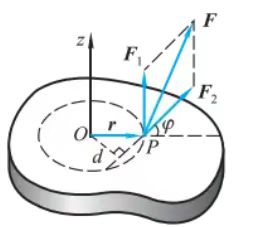
\includegraphics[width=0.3\linewidth]{images/力矩}
	\caption[定轴转动的力矩]{}
	\label{fig:}
\end{figure}
$\mathbf{F_1}$为平行于转轴的力，$\mathbf{F_2}$为垂直于转轴的力，d成为力臂。
$$ |\mathbf{M_z}|=|\mathbf{F_2}\mathbf{r}\sin\varphi|=|\mathbf{F_2}d|$$

\subsection{角速度}

1.角速度为\textbf{矢量}，$\mathbf{v}=\mathbf{\omega}\mathbf{r} $

2.角速度的方向用右手螺旋定则判断，且对于定轴转动，角速度方向始终与转轴平行。

\subsection{转动惯量和定轴转动定律}

下给出简要推导：

取刚体中任一质量元$\Delta m$,其受外力为$\mathbf{F_{ei}}$,受内力为$\mathbf{F_{i}}$

由牛顿第二定律$$\mathbf{F_{ei}}+\mathbf{F_{i}} ={\Delta m}\mathbf{a_i}$$

在自然坐标系中$${F_ei}\sin\varphi_i+F_{i}\sin\theta_i= \Delta m\mathbf{r_i}\mathbf{\alpha}$$

同乘$\mathbf{r_i}$，并对质量元累加$$\sum_{i=1}^{n}{F_{ei}}\sin\varphi_i+\sum_{i=1}^{n}F_{i}\sin\theta_i=\sum_{i=1}^{n}\Delta m_i{r_i}^2\alpha$$

对于刚体而言，内力作用产生的相对位移为0，因此内力矩之和为零。

因此$$\mathbf{M_z}=J\mathbf{\alpha}=J\dfrac{\mathrm{d\omega}}{\mathrm{d}t}$$
\begin{figure}[h]
	\centering
	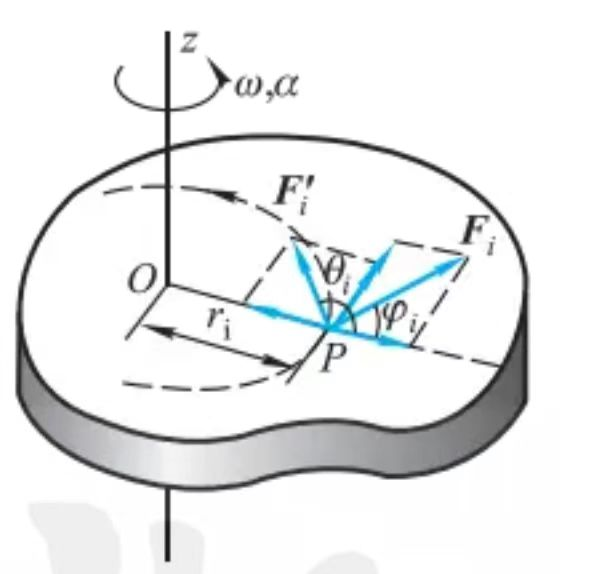
\includegraphics[width=0.3\linewidth]{images/定轴转动定律}
	\caption{定轴转动定律}
	\label{fig:}
\end{figure}

\subsubsection{转动惯量}

1.$J=\sum_{i=1}^{n}\Delta m_i{r_i}^2 $，单位为$kg\cdot m^2$

2.当刚体为质量连续体时，$J=\int r^2\mathrm{d}m $(其中r为质元$\mathrm{d}m $到轴的距离)

3.转动惯量取决于刚体的形状大小、质量分布和转轴的位置。

\subsubsection{转动与平动的联系}

对比牛顿第二定律和定轴转动定律
$\left\{
\begin{aligned}
	\mathbf{F}=m\mathbf{a}\\
	\mathbf{M}=\mathbf{J}\alpha
\end{aligned}
\right.$

其中，m成为惯性质量，是平动惯性的量度，而$\mathbf{J}$也可视作定轴转动刚体的一种特性，是刚体转动惯量的量度；且牛顿第二定律两边同乘$\mathbf{r}$,即为定轴转动定律，因此，可将定轴转动定律视作转动下的牛顿第二定律。

\subsubsection{平行轴定理}

\textbf{刚体对任一转轴的转动惯量$\mathbf{J}$等于通过质心轴的转动惯量$\mathbf{J_c}$加上$\mathbf{mh^2}$,其中$\mathbf{h}$ 为两平行轴之间的距离。}

$$\mathbf{J}=\int(x+h)^2\mathrm{d}m=\int x^2\mathrm{d}m+\int h^2\mathrm{d}m+2h\int x\mathrm{d}m=\mathbf{J_c}+mh^2 $$

(当刚体是绕定轴转动的匀质对称刚体时，$\int x\mathrm{d}m=0 $)

\subsubsection{常见模型的转动惯量}

下给出薄圆盘的转动惯量证明，刚体的转动惯量一般都可由一般模型和平行轴定理推导而得。

圆盘的质量为m,半径为R,设圆盘面密度为$\sigma$，则$\sigma=\dfrac{m}{\pi R^2}$,取宽度为$\mathrm{d}r $的圆环，则有该圆环质量$\mathrm{d}m=(2\pi r)\mathrm{d}r$,则
$$\mathbf{J}=\int r^2\mathrm{d}m=\int_{0}^{R}2\pi\sigma r^3\mathrm{d}r=\dfrac{\pi\sigma R^4}{2}=\frac{1}{2}mR^2$$

\begin{figure}[h]
	\centering
	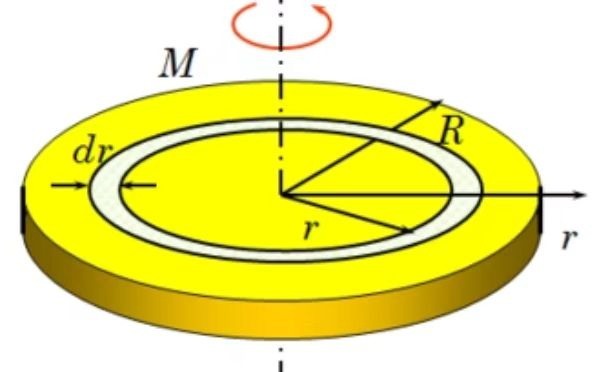
\includegraphics[width=0.2\linewidth]{images/薄圆盘转动惯量}
	\caption[薄圆盘转动惯量]{}
	\label{fig:}
\end{figure}
下为常见刚体转动惯量（书P118-119)
\begin{figure}[h]
	\centering
	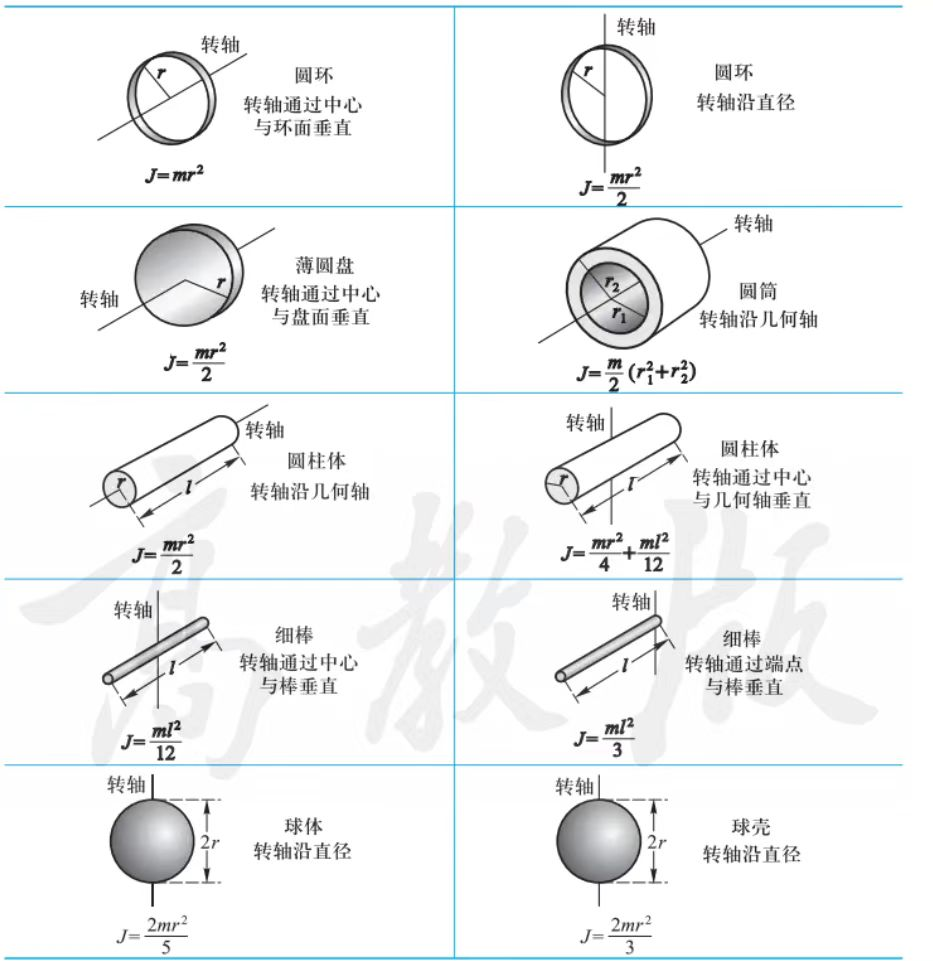
\includegraphics[width=0.9\linewidth]{images/转动惯量模型}
	\caption[转动惯量模型]{}
	\label{fig:}
\end{figure}

% 
\section{定轴转动中的功能关系}

\begin{definition}[力矩的功]
	
刚体定轴运动中，外力做功仅包括垂直转轴平面内分量。

已知力矩 $M_i  = F_irisin\phi \qquad$  角位移为$ \theta \qquad$

则合外力做功为$$A = \sum A_i = \sum \int_{\theta_0}^{\theta} M_i d\theta = \int_{\theta_0}^{\theta}(\sum M_i)d\theta = \int_{\theta_0}^{\theta}Md\theta \qquad $$ 
式中 $M = \sum M_i$ 为刚体所受到的合外力矩。

\end{definition}

\begin{definition}[刚体转动惯量]
$J = \sum m_ir_i^2$
\end{definition}

\begin{definition}[刚体转动动能]
$E_k = \frac{1}{2} J \omega^2$
\end{definition}

\begin{definition}[刚体定轴转动动能定理]
合外力矩对刚体所做的功等于刚体动能增量
\end{definition}
\begin{supplement}
工程上的应用：转动惯量很大的飞轮储存转动动能
\end{supplement}



% \section{进动与流体}
\begin{definition}[进动]
    \textbf{进动}是指刚体绕轴旋转时，旋转轴绕另外一个轴旋转的回转现象，如图\ref{pic:3.5-1}所示.
\end{definition}
\begin{figure}[hb]
    \begin{center}
        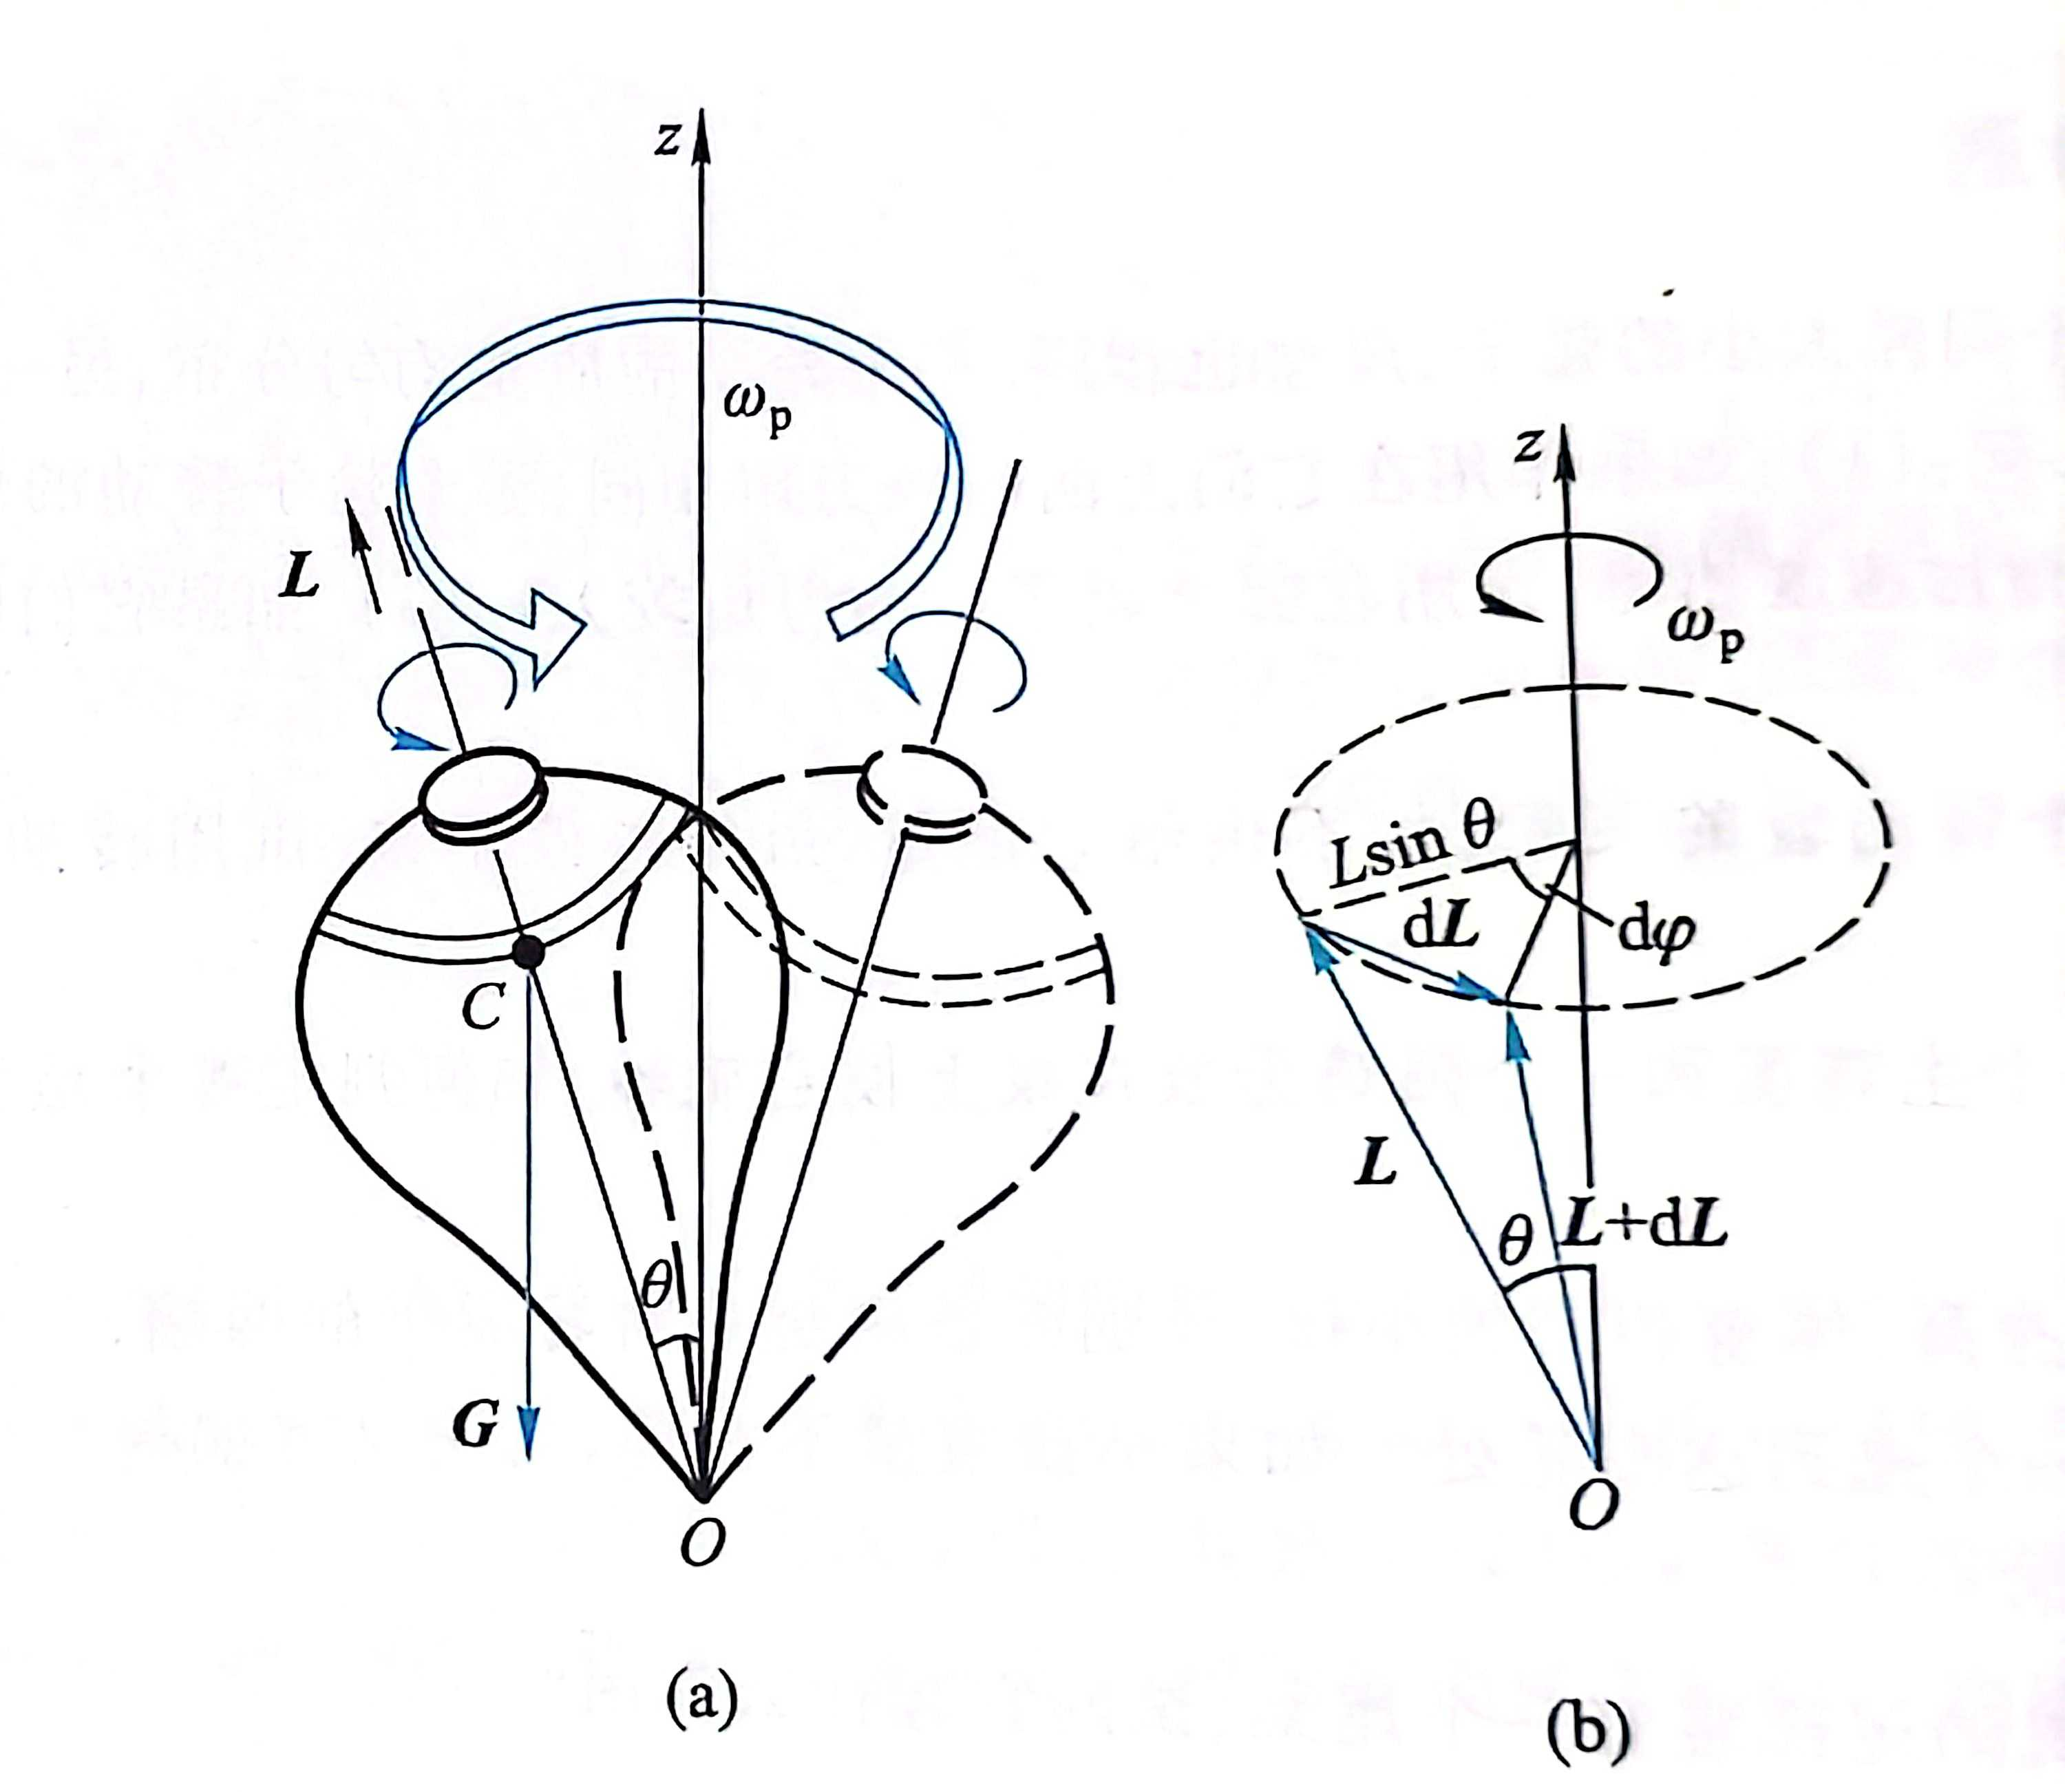
\includegraphics[width=0.6\textwidth]{images/3-5-1.jpg}
        \caption{进动示意图}
        \label{pic:3.5-1}
    \end{center}
\end{figure}

进动是由作用在刚体上与旋转轴垂直的外力矩引起的，一般出现在自转角速度较大的情况下.进动角速度可由公式\ref{equ:3.5-1}确定.

\begin{equation}
    \omega_p=\dfrac{M}{J\omega \sin\theta}
    \label{equ:3.5-1}
\end{equation}

在自转角速度较小的情况下，刚体可能还会\textbf{章动}，在此不详细介绍.

\begin{definition}[定常流动]
    流场中各点流速不随时间变化的流动称为\textbf{定常流动}.
\end{definition}

对于不可压缩，没有黏性的\textbf{理想流体}，有伯努利方程，表明作定常流动的流体中，在同一流管中任何一点处，流体每单位体积的动能和势能以及在该处的压强之和为常量.在工程中，该方程常表示为公式\ref{equ:3.5-2}.
\begin{equation}
    \dfrac{p}{\rho g}+\dfrac{v^2}{2g}+h=Const
    \label{equ:3.5-2}
\end{equation}
其中，公式\ref{equ:3.5-2}左端各项依次称为压力头（表征压力）、速度头（表征动能）、水头（表征势能），公式右端表示一个（具有长度量纲的）常数.
% \part{近代物理}
\chapter{狭义相对论}
\section{伽利略相对性原理~伽利略变换}

\subsection{伽利略相对性原理}

\textbf{根据实验现象可以得出，力学规律对于一切惯性系都是等价的。}

\subsection{伽利略变换}

事件：某一时刻发生在空间某一点的一个事例。

设两个惯性系S系和S'系，且S'系相对于S系以速度$\mathbf{u}$沿X轴方向做匀速直线运动。

如果某时刻在空间某一点P发生了一事件，S和系的观测者分别观测这一事件，且规定当S系和S'系中原点重合时，两惯性系开始计时，即$t_{0}=t'_{0}$。

则可以得到正变换
$\left\{
\begin{aligned}
	x'=x-\mathbf{u}t\\
	y'=y\\
	z'=z\\
	t'=t
\end{aligned}
\right.$

和负变换
$\left\{
\begin{aligned}
	x=x'+\mathbf{u}t'\\
	y=y'\\
	z=z'\\
	t=t'
\end{aligned}
\right.$

\subsection{经典力学时空观}

1.时间绝对性:时间间隔与惯性系选择无关。

2.空间绝对性:空间间隔与惯性系选择无关。

3.时间、长度、质量是绝对的，同时性是绝对的，坐标和速度是相对的。
% \section{狭义相对论基本原理与洛伦兹变换}
\subsection{狭义相对论基本原理}
成立前提：在彼此相对作匀速直线运动的\textbf{惯性参考系}中。

\begin{enumerate}
	\item \textbf{相对论原理：}物理定律在一切惯性参考系中都具有相同的数学表达形式。（所有惯性参考系对于描述物理现象都是等价的）
	\item \textbf{光速不变原理：}在彼此相对作匀速直线运动的任一惯性参考系中，所测得的光在真空中的传播速度都是相等的。
\end{enumerate}

\subsection{洛伦兹变换}
反映了两个相对作匀速直线运动的惯性参考系中的时空变换关系。

变换关系满足
$$\begin{cases}
	x^{'}=\frac{x-ut}{\sqrt{1-(\frac{u}{c})^2}}\\
	y^{'}=y\\
	z^{'}=z\\
	t^{'}=\frac{t-\frac{ux}{c^2}}{\sqrt{1-(\frac{u}{c})^2}}
\end{cases}$$
或
$$\begin{cases}
	x=\frac{x^{'}+ut}{\sqrt{1-(\frac{u}{c})^2}}\\
	y=y^{'}\\
	z=z^{'}\\
	t=\frac{t^{'}+\frac{ux}{c^2}}{\sqrt{1-(\frac{u}{c})^2}}
\end{cases}$$
\begin{enumerate}
	\item 洛伦兹变换与伽利略变换：当$u\ll c$时，即比值$\beta=\frac{u}{c}$很小时，洛伦兹变换变换就转化为伽利略变换。
	\item 相对论并没有把经典力学推翻，只是揭示了它的局限性。
	\item 相对论指出物体的速度不能超过真空中的光速。
\end{enumerate}

% 
	
	
\section{相对论速度变换}
	
\begin{theorem}[相对论速度变换公式]


令$\beta= \frac{u}{c}$

依据：洛伦兹坐标变化

当物体沿X方向运动时，K系中速度表达式为
$$v_x = \frac{dx}{dt}	$$
K'系中速度表达式为
$$v'_x = \frac{dx'}{dt'} =  \frac{dx'-udt}{dt'-\frac{u}{c^2}dx} =\frac{v_x-u}{1-\frac{u}{c^2} v_x}	$$

$$v'_y =\frac{V_y(1-\beta^2)^\frac{1}{2}}{1-\frac{u}{c^2}v_x}	$$


逆变换

$$ v_x = \frac{v'_x + u} {1 + \frac{u} {c^2}v'_x } $$

$$v_y =\frac{v_y'(1-\beta^2)^\frac{1}{2}}{1+\frac{u}{c^2}v_x'}	$$

$v_z$和$v_y$同理
\end{theorem}

\begin{note}
	适用范围：$u$(惯性系间相对速度)和$v$接近光速时。
	
	相对论速度变换遵循光速不变原理。
\end{note}



% \part{电磁学}
\chapter{静电场}
\section{电荷~库仑定律}

\subsection{电荷}

1.\textbf{电荷量}：表示物体所带电荷多寡的物理量。

2.物体所带电荷只有正电荷和负电荷,同号电荷相互排斥，异号电荷相互吸引。

\subsection{电荷守恒定律}

1.\textbf{起电}：通过某种作用，使该物体内电子不足或过多而呈带电状态。

2.\textbf{电荷守恒定律}：在一个与外界没有电荷交换的系统内，无论经过怎样的物理过程，系统内正、负电荷的代数和总保持不变。

3.电荷是相对论不变量，即电荷量与运动无关。

\subsection{电荷的量子化}

电荷量这种只能取分立的、不连续量值的性质，称为电荷量子化。

一般近似取$e=1.602176634×10^{-19}$

\subsection{库仑定律}

1.库仑扭秤实验总结出了\textbf{库仑定律}：两个静止点电荷之间相互作用力的大小与这两个点电荷的电荷$q_{1}$和$q_{2}$的乘积成正比，而与这两个点电荷之间的距离$r_{12}$的二次方成反比，作用力的方向，沿着这两个点电荷的连线。

$$\mathbf{F}=k\frac{q_{1}q_{2}}{{r_{12}}^{2}}$$
$$k=\frac{1}{4\pi\varepsilon_{0}}$$
则$$\mathbf{F_{12}}=\mathbf{F_{21}}=\frac{1}{4\pi\varepsilon_{0}}\frac{q_{1}q_{2}}{{r_{12}}^{2}}\mathbf{e_{r_{12}}} $$

2.适用条件：真空、静止、点电荷

\subsection{静电力的叠加原理}

1.\textbf{静电力叠加原理}：当空间有两个以上的点电荷时，作用在某一点电荷上的总静电力等于其他各点电荷单独存在时，对该点电荷所施静电力的矢量和。

$$\mathbf{F}=\sum_{i=1}^{n}\mathbf{F_{i}}=\frac{1}{4\pi\varepsilon_{0}}\sum_{i=1}^{n}\frac{qq_{i}}{{r_{i}}^{2}}\mathbf{e_{r_{i}}}$$

2.库伦定律只适用于点电荷,将带电体看作是由许多电荷元组成的，根据库仑定律和叠加原理，则可求解带电体之间的相互作用力。

% \section{静电场\quad 电场强度}
\subsection{电场}
电场：电荷周围存在的一种特殊物质。分布在一定范围的空间里，具有能量、动量等属性，并通过交换场量子来实现相互作用的传递。电磁场的媒介子是光子。

电场力：电场对处在其中的其他电荷的作用力。两个电荷之间的相互作用力本质上是一个电荷的电场作用在另一个电荷上的电场力。

静电场：相对于观察者为静止的点电荷在其周围所激发的电场。

\subsection{电场强度}
\subsubsection{检验电荷}
\begin{enumerate}
	\item 所带电荷量充分小。
	\item 线度小到可以被看作点电荷。
\end{enumerate}
用检验电荷所受的力与检验电荷所带电荷量之比，可以定义电场强度。

\subsubsection{电场强度}
定义：电场中某点的电场强度的大小等于单位电荷在该点所受的力的大小，其方向为正电荷在该点的受力方向。
$$\vec{E}=\frac{\vec{F}}{q_0}$$

符号：$\vec{E}$

单位：$N/C$，$V/m$

标矢性：矢量

\subsection{电场强度的叠加原理}
点电荷系在空间任一点所激发电场的总电场强度等于各个点电荷单独存在时在该点各自所激发电场的电场强度的矢量和。（简称场强叠加原理）

利用这一原理可以计算任意带电体所激发电场的电场强度，因为任何带电体都可以看作许多点电荷的集合。

\subsection{电场强度的计算}
\subsubsection{点电荷}
对于一个静止的点电荷$q$（场源电荷），距$q$为$r$的$P$点（场点）的电场强度为
$$\vec{E}=\frac{1}{4\pi\varepsilon_0}\frac{q}{r^2}\vec{e_r}$$

式中$\vec{e_r}$是由点电荷$q$指向$P$点的单位矢量。

\subsubsection{点电荷系}
$$\vec{E}=\vec{E_1}+\vec{E_2}+\dots+\vec{E_n}=\sum_{i=1}^n{\frac{q_i}{4\pi\varepsilon_0 r_i^2}\vec{e_ri}}$$

\subsubsection{连续分布电荷}
把带电体看成许多极小的连续分布的电荷元$\mathbf{d}q$的集合，每一个电荷元$\mathbf{d}q$都当作点电荷来处理。
$$\mathbf{d}\vec{E}=\frac{1}{4\pi\varepsilon_0}\frac{\mathbf{d}q}{r^2}\vec{e_r}$$
$$\vec{E}=\int\mathbf{d}\vec{E}=\frac{1}{4\pi\varepsilon_0}\int\frac{\mathbf{d}q}{r^2}\vec{e_r}$$

\subsubsection{经典模型}
\begin{itemize}
	\item 电偶极子
	
	电偶极子：两个大小相等符号相反的点电荷$+q$和$-q$，当它们之间的距离$l$比所考虑的场点到它们的距离小得多时，这一电荷系统称为电偶极子。
	
	轴线：取从负电荷指向正电荷的矢量$\vec{l}$的方向作为轴线的正方向。
	
	电偶极矩（电矩）：$\vec{p}=q\vec{l}$
	
	对轴线的延长线上的某点A：$\vec{E_A}=\frac{1}{4\pi\varepsilon_0}\frac{2\vec{p}}{y^3}$
	
	对中垂线上的某点A：$\vec{E_A}=-\frac{1}{4\pi\varepsilon_0}\frac{\vec{p}}{x^3}$
	
	\item  均匀带电直棒
	
	长度为$L$，总电荷量为$q$，电荷线密度$\lambda=q/L$。棒外一点$P$离开直棒的垂直距离为$a$，$P$点和直棒两端的连线与直棒之间的夹角分别是$\theta_1$和$\theta_2$。
	
	$P$点的电场强度：$E=\frac{\lambda}{4\pi\varepsilon_0}\sqrt{2-2\cos(\theta_1-\theta_2)}$，与$Ox$轴的夹角$\alpha=\arctan\frac{\cos\theta_1-\cos\theta_2}{\sin\theta_2-\sin\theta_1}$
	
	无限长均匀带电直棒（或$a\ll L$时）：$E=\frac{\lambda}{4\pi\varepsilon_0}$（$\theta_1=0$，$\theta_2=\pi$）
	
	\item 带电圆环
	
	半径为$R$，总电荷量为$q$。
	
	轴线上一点$P$处的电场强度：$E=\frac{qx}{4\pi\varepsilon_0(x^2+R^2)^{3/2}}$。若$q$为正电荷，沿$Ox$轴正方向：若$q$为负电荷，沿$Ox$轴负方向。
	
	当$x\gg R$时：$E=\frac{q}{4\pi\varepsilon_0 x^2}$
	
	\item 带电圆盘
	
	半径为$R$，面密度为$\sigma$。
	
	轴线上一点$P$处的电场强度：$E=\frac{\sigma}{2\varepsilon_0}(1-\frac{x}{\sqrt{R^2+x^2}})$。若$\sigma>0$，沿$Ox$轴正方向；若$\sigma<0$，沿$Ox$轴负方向。
	
	当$R\gg x$时：：$E=\frac{\sigma}{2\varepsilon_0}$
	
	当$x\gg R$时：$E=\frac{q}{4\pi\varepsilon_0 x^2}$
\end{itemize}

\subsection{电场对电荷的作用力}
$$\vec{F}=q\vec{E}$$
$q>0$时，$\vec{F}$与$\vec{E}$同向；$q<0$时，$\vec{F}$与$\vec{E}$反向。

\subsection{电场线\quad 电场强度通量}
\subsubsection{电场线}
 电场线上每一点的切线方向都与该点处的电场强度$\vec{E}$的方向一致。任一点电场线的密度与该点的电场强度的大小成正比。
 
 \begin{enumerate}
 	\item 电场线起始于正电荷（或来自无穷远处），终止于负电荷（或伸向无穷远处），不会在没有电荷的地方中断（电场强度为零的奇异点除外）。
 	\item 电场线不能形成闭合曲线。
 	\item 任何两条电场线不会相交。
 \end{enumerate}
 
 \subsubsection{电场强度通量}
 定义：在均匀电场中取一个想象中的平面。引入面积矢量$\vec{S}$，其大小等于平面的面积$S$，其方向为平面正法线的方向。设平面正法线的单位矢量$\vec{e_n}$与$\vec{E}$成$\theta$角。
 
 如果取电场线的密度等于场强的大小，则通过这一平面的电场线总数等于
 $$\varPhi_e=E\cos\theta S=\vec{E}\cdot\vec{S}$$
 也称作通过该面积的电场强度通量，即$\vec{E}$通量。
 
 \begin{itemize}
 	\item 不均匀电场：
 	
 	把曲面划分为无限多个面积元$\mathbf{d}S$，在每一个无限小的面积元$\mathbf{d}S$上电场强度可以认为是均匀的。
 	$$\varPhi_e=\int_{S}\mathbf{d}\varPhi_e=\int_{S}\vec{E}\cdot\mathbf{d}\vec{S}$$
 	
 	\item 闭合曲面：
 	
 	对非闭合曲面，面法线的方向可以取曲面的任一侧。对闭合曲面来说，通常规定自内向外的方向为面积元法线的正方向。
 	
 	所以，在电场线从曲面之内向外穿出时$\vec{E}$通量为正：反之，在电场线从外部穿入曲面时，$\vec{E}$通量为负。
 \end{itemize}
% 
	
	
	\section{静电场的高斯定理}
	
	\begin{definition}[高斯定理]
		在静电场中，通过任意闭合曲面的电场强度通量等于该曲面内电荷量的代数和除以$\varepsilon _{0}$
		
		$$\oint _{S}E\cdot dS=\frac{1}{\varepsilon _{0}}\sum _{i}q_{i}$$
		
	\end{definition}
	
	\begin{note}
		
		闭合球面上的$E$通量与球面所围成的电荷量成正比，与半径无关。
		
		高斯定理说明了电场强度对闭合面通量和场源电荷关系。
		
		闭合曲面外电荷对闭合曲线上各个点电场强度有作用，但对闭合曲面整体$E$通量贡献为$0$。
		
		适用范围：静电场、运动电荷、迅速变化的电场。
	\end{note}
	
应用方法：

一、电荷分布具有某些特殊的对称性，使相应的电场分布具有一定对称性：
\begin{example}
	1:球对称性：点电荷、均匀带点球体。2：轴对称性：均匀带电直线、柱。3：平面对称性：无限大均匀带点平板。
\end{example}

二、高斯面选择要求：

	电场强度垂直于闭合面且大小处处相等/一部分电场强度垂直于闭合面且处处相等，另一部分电场强度与闭合面平行。

\begin{example}
	球对称电场：球半径为R
	
1、$q$均匀分布在整个球体
	
（1）$P$点在球内
	
$$E = \frac{q}{4\pi\varepsilon _{0}r^2}e_r$$

（2）$P$点在球外

$$E = \frac{qr}{4\pi\varepsilon _{0}R^3}e_r$$
2、$q$均匀分布在球面上
（1）$P$点在球内

$$E =0$$

（2）$P$点在球外

$$E = \frac{qr}{4\pi\varepsilon _{0}R^3}e_r$$


\end{example}

\begin{example}
	柱对称电场：
	
（1）$P$点在圆柱内

$$ E=\frac{\lambda}{2\pi \varepsilon _{0}r}e_{r}$$

（2）$P$点在圆柱外

$$E =\frac{\lambda r}{2\pi \varepsilon _{0}R^2}e_{r}$$
\end{example}

\begin{example}
	平面对称电场：
	
$$E = \frac{\sigma}{2\varepsilon_0} e_n$$

一对电荷面密度相等异号的均匀带电无限大电场（电容板）电场强度大小为

$$E = \frac{\sigma}{\varepsilon_0} $$
\end{example}


% \section{电场强度与电势的关系}
电场强度与电势的积分关系即为电势与电势差（电压）的定义式（取无穷远处为零势点时可以表示为公式\ref{equ:7.5.1}与公式\ref{equ:7.5.2}）.
\begin{equation}
    V_a=\dfrac{W_a}{q_0}=\int_{a}^{\infty}\bm{E}\cdot \mathrm{d}\bm{l}
    \label{equ:7.5.1}
\end{equation}
\begin{equation}
    U_{ab}0=V_a-V_b=\dfrac{W_a}{q_0}-\dfrac{W_b}{q_0}=\int_{a}^{b}\bm{E}\cdot \mathrm{d}\bm{l}
    \label{equ:7.5.2}
\end{equation}

电场强度与电势的微分关系可以由电场力做功推导，结论是静电场中某点的电场强度在量值上等于该点电势梯度的大小，方向与电势梯度矢量方向相反.换言之，\textbf{电场强度的方向为该点电势降低最快的方向}.公式\ref{equ:7.5.3}给出了这个结论的数学表达.
\begin{equation}
    \bm{E}=-\nabla V=-\dfrac{\mathrm{d}V}{\mathrm{d}\bm{n}}\bm{e}_n=-\mathrm{grad}V
    \label{equ:7.5.3}
\end{equation}

公式\ref{equ:7.5.3}的分量式的意义是：在静电场中，电场强度在任一方向的分量等于该方向电势变化率的负值.
% \section{静电场中的导体}
\subsection{静电平衡}
将不带电的金属导体置于电场中，由静电感应现象在表面产生感应电荷，感应电荷不断积累，产生附加电场，最终达到导体内部电场强度处处为零，导体中没有任何电荷作定向运动，此状态称为\textbf{静电平衡}状态.需要注意的是该状态是没有电荷作定向运动而非没有电荷作运动，因为存在分子热运动.建立静电平衡的过程如图\ref{pic:7-6-1}所示.
\begin{figure}[hb]
    \begin{center}
        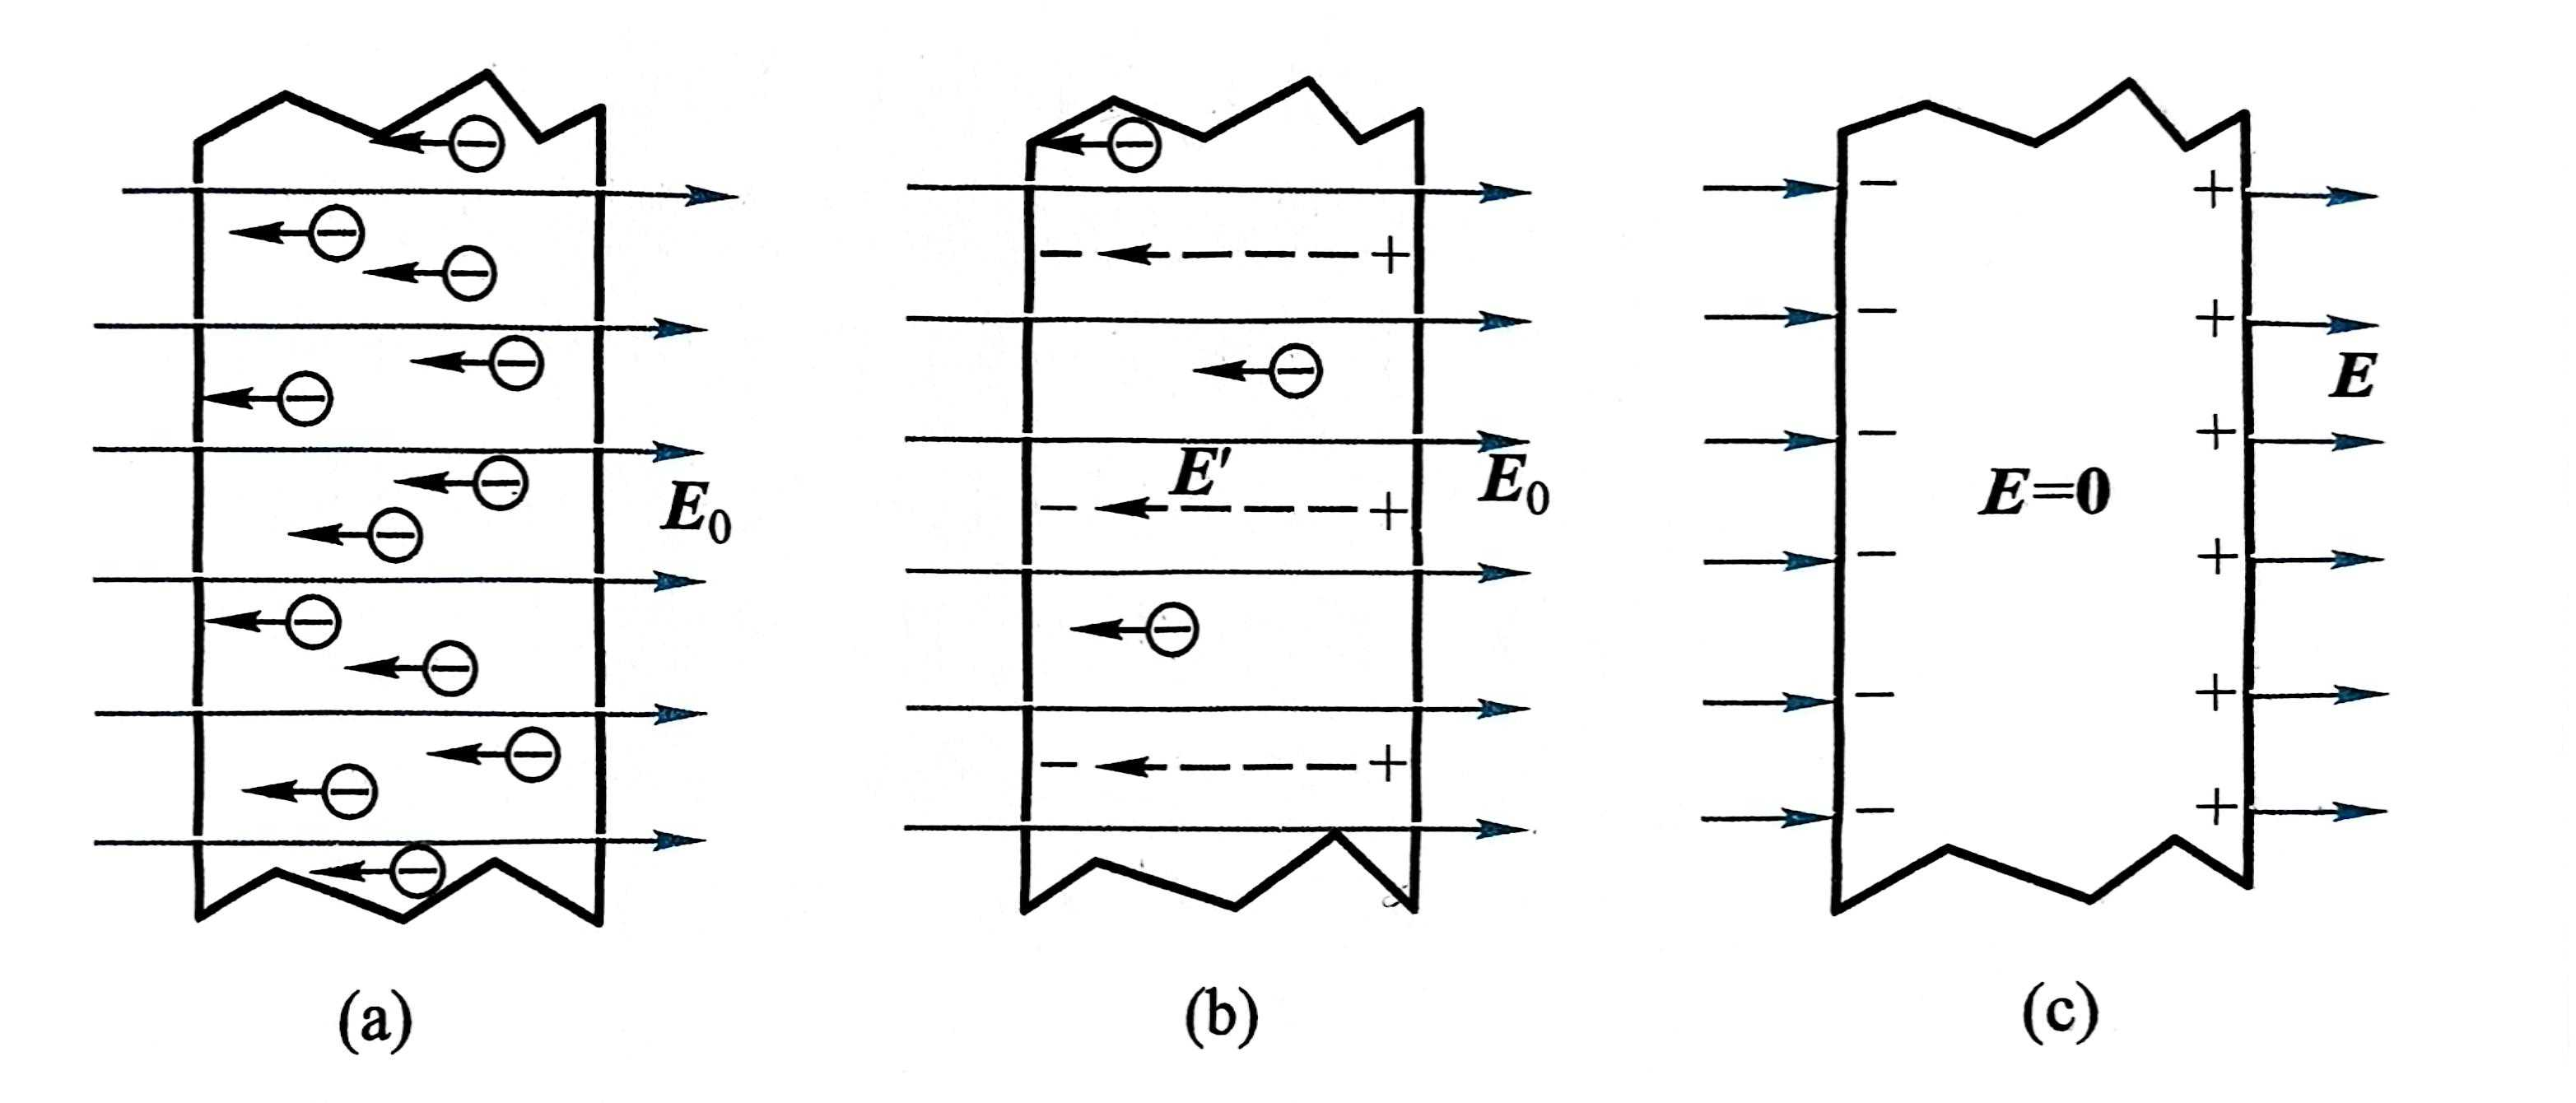
\includegraphics[width=0.6\textwidth]{images/7-6-1.jpg}
        \caption{静电感应过程}
        \label{pic:7-6-1}
    \end{center}
\end{figure}

根据导体静电平衡的条件，如图\ref{pic:7-6-2}所示，我们有以下推论：
\begin{enumerate}
    \item 导体是等势体，其表面是等势面.
    \item 导体表面的电场强度垂直于导体表面.
\end{enumerate}

\begin{figure}[hb]
    \begin{center}
        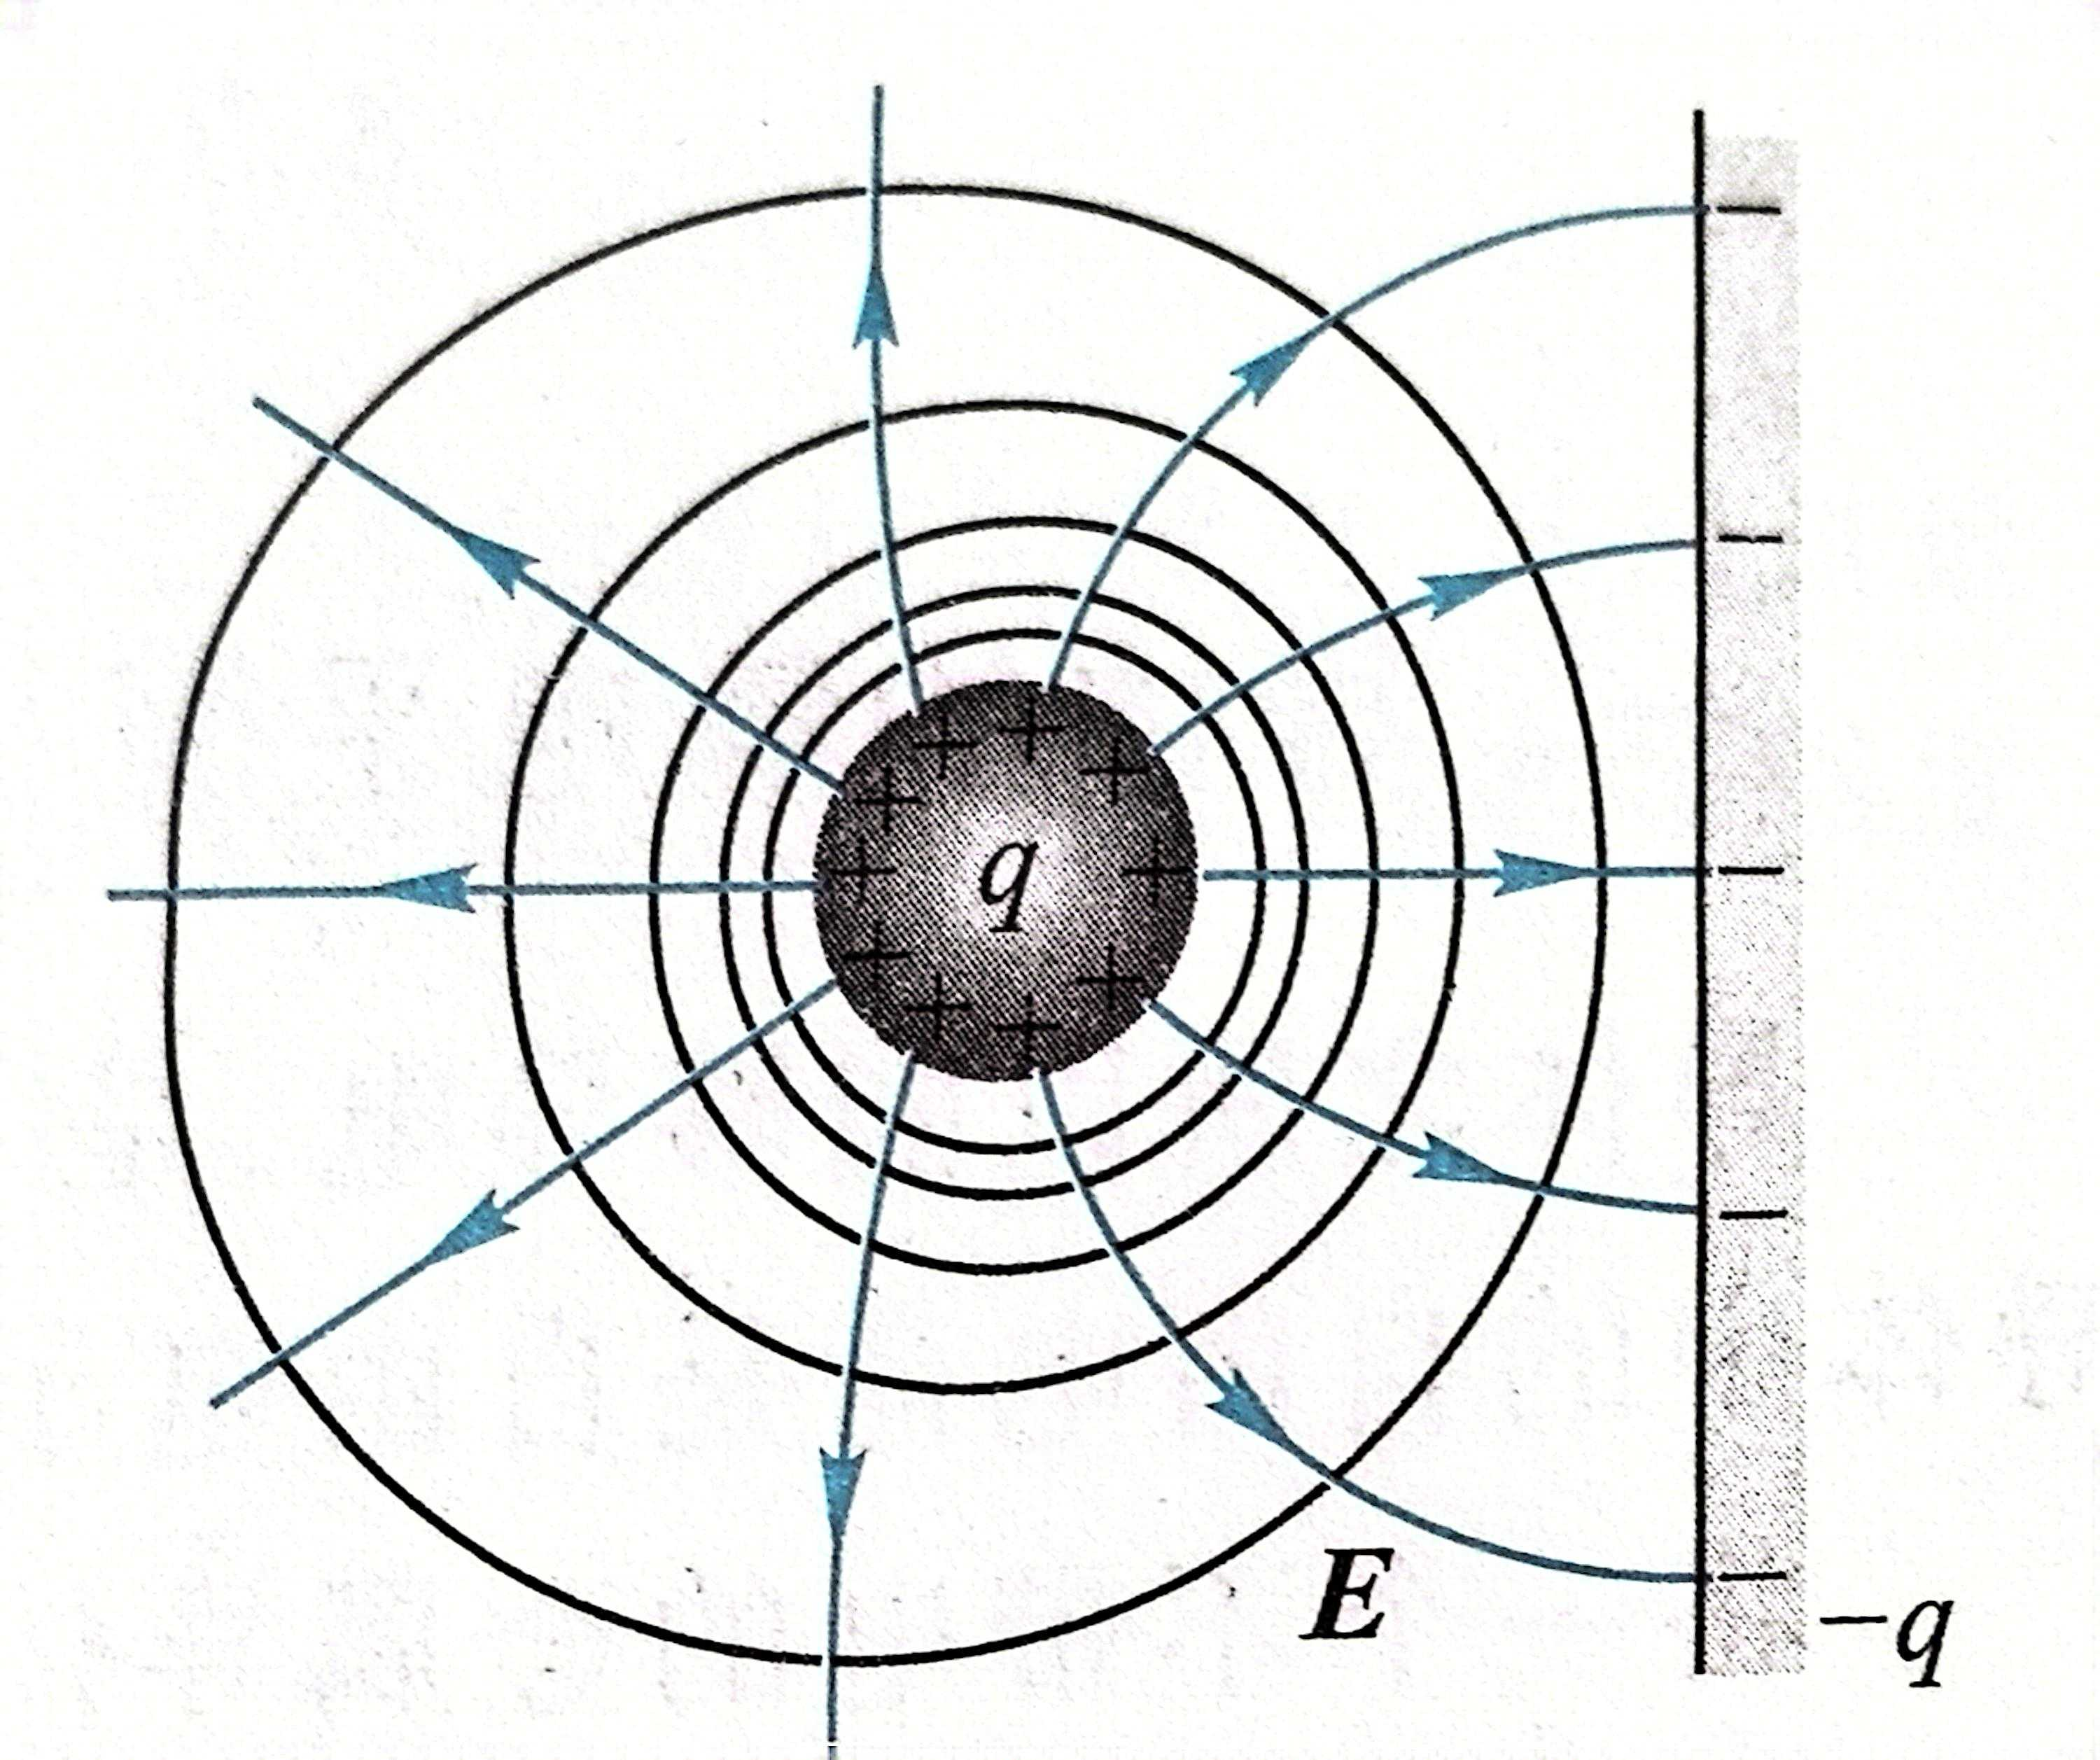
\includegraphics[width=0.4\textwidth]{images/7-6-2.jpg}
        \caption{导体附近电场/等势面分布}
        \label{pic:7-6-2}
    \end{center}
\end{figure}

\subsection{静电平衡时导体上的电荷分布}
根据高斯定理，当带点导体处于静电平衡状态时，电荷只能分布于导体的表面上（仅有感应电荷）.如果导体有空腔，空腔内有电荷时，导体内表面带有与电荷电量相等电性相反的感应电荷；空腔内没有电荷时，导体只有外表面带有感应电荷.


如图\ref{pic:7-6-3}方式取高斯面，由高斯定理，有带电导体表面附近的电场强度公式
\[
\bm{E}=\dfrac{\sigma}{\epsilon_0}\bm{e}_n
\]
\begin{figure}[h]
    \begin{center}
        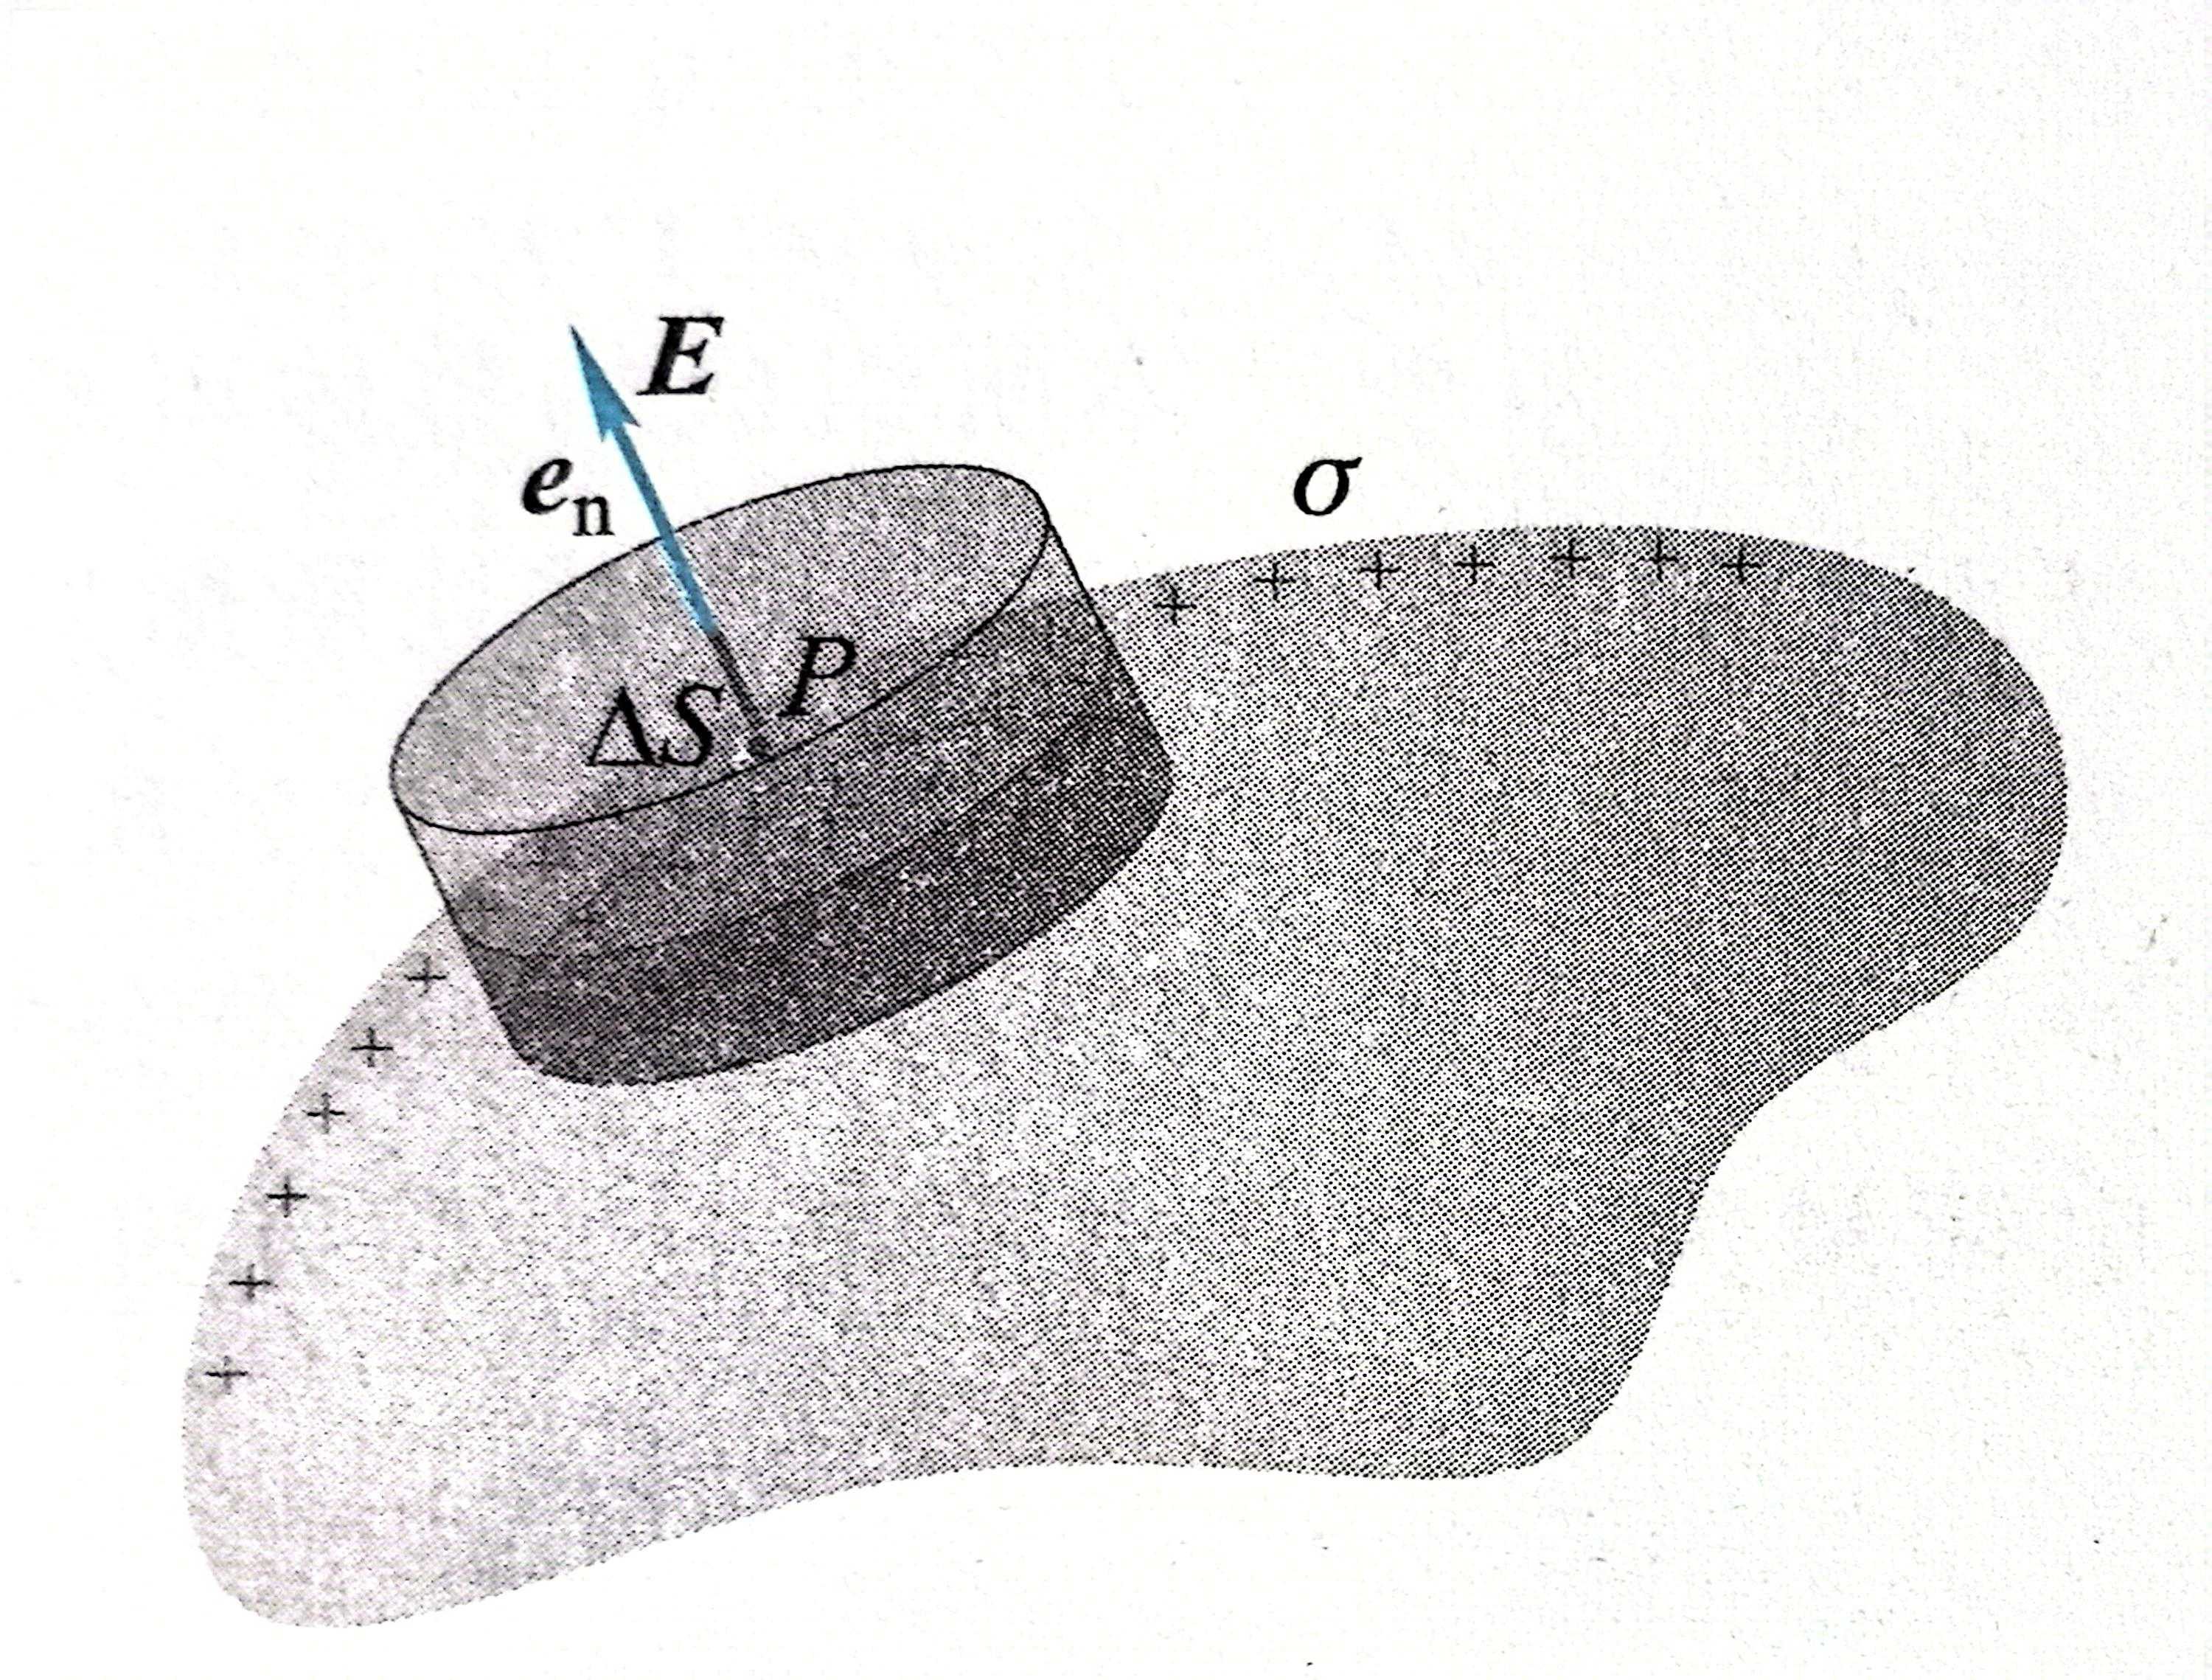
\includegraphics[width=0.4\textwidth]{images/7-6-3.jpg}
        \caption{导体表面附近的高斯面取法}
        \label{pic:7-6-3}
    \end{center}
\end{figure}
\begin{attention}{ }{7.6.1} % 添加标签参数
不要将该公式与无限大均匀带电平面产生的电场强度混淆！事实上，这两个公式说明的是一个问题，只不过电荷面密度代表的含义有所差别.
\end{attention}

对于孤立的带电导体，感应电荷在其表面的分布由其表面曲率确定.曲率越大，电荷分布越密集，此处曲率的符号表征“大小”.只有孤立导体球表面电荷分布均匀.

\subsection{静电屏蔽}
在静电平衡的条件下，导体空腔外的带电体不会影响腔内的电场分布；接地的空腔导体腔内电荷不会影响腔外的电场分布.这就是\textbf{静电屏蔽}效应.
% \section{电容器的电容}

\subsection{孤立导体的电容}

1.\textbf{孤立导体的电容}:从理论及实验可知,一个孤立导体的电势V与他所带的电荷量q呈线性关系。
$$C=\frac{q}{V}$$

2.他只与导体的大小、形状和周围介质有关。

3.电容是表征导体储电能力的物理量，其物理意义是使导体升高单位电势所需的电荷量，单位：法拉F。

4.孤立导体球半径为R，带电荷为q，则它的电容为$C=\frac{q}{V}=4\pi\varepsilon_{0}R$。

\subsection{电容器的电容}

根据静电屏蔽的原理，用一个封闭的导体壳B将导体A包围起来，使得导体A及导体壳B构成的一对导体系的电势差$V_{A}-V_{B}$不再受到壳外导体的影响，从而维持恒定，这样一个导体系可以称为电容器。

\begin{figure}[h]
	\centering
	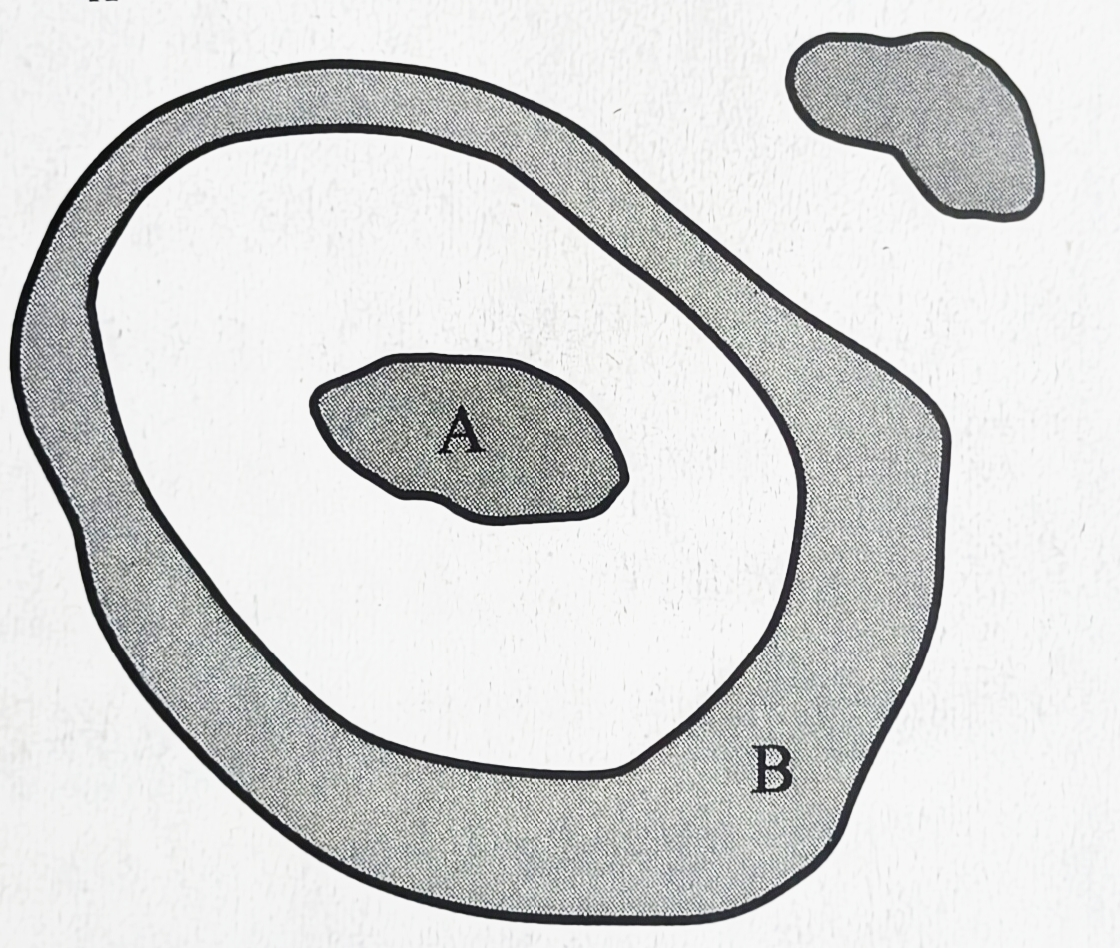
\includegraphics[width=0.3\linewidth]{images/电容器}
	\caption{电容器}
	\label{fig:}
\end{figure}

1.\textbf{电容器的电容}:两导体极板表面上均带有的等量异号电荷q与两极板电势差$\Delta V$的比值。
$$C=\frac{q}{V_{A}-V_{B}}$$

2.实验证明：充有电介质的电容器电容为两板间为真空时的电容$C_{0}$的$\varepsilon_{r}$倍。

其中$\varepsilon_{r}$称为介质的相对电容率或相对介电常量，量纲为1。

\subsection{常见电容器的电容}

\subsubsection{平行板电容器}

两板所带电荷量为q，板间距为d，面积为S，中间充有相对介电常量$\varepsilon_{r} $的电介质，极板的电荷面密度为$\sigma_{0}$。

$$Q=\sigma_{0}S$$

由高斯定理$$D=\sigma_{0}$$

则有$$E=\frac{\sigma_{0}}{\varepsilon_{0}\varepsilon_{r}}$$
$$U=Ed=\int E\mathrm{d}\mathbf{l}$$
$$C=\frac{q}{U}=\frac{\varepsilon_{0}\varepsilon_{r}S}{d}=\varepsilon_{0}\varepsilon_{r}C_{0}$$
\begin{figure}[h]
	\centering
	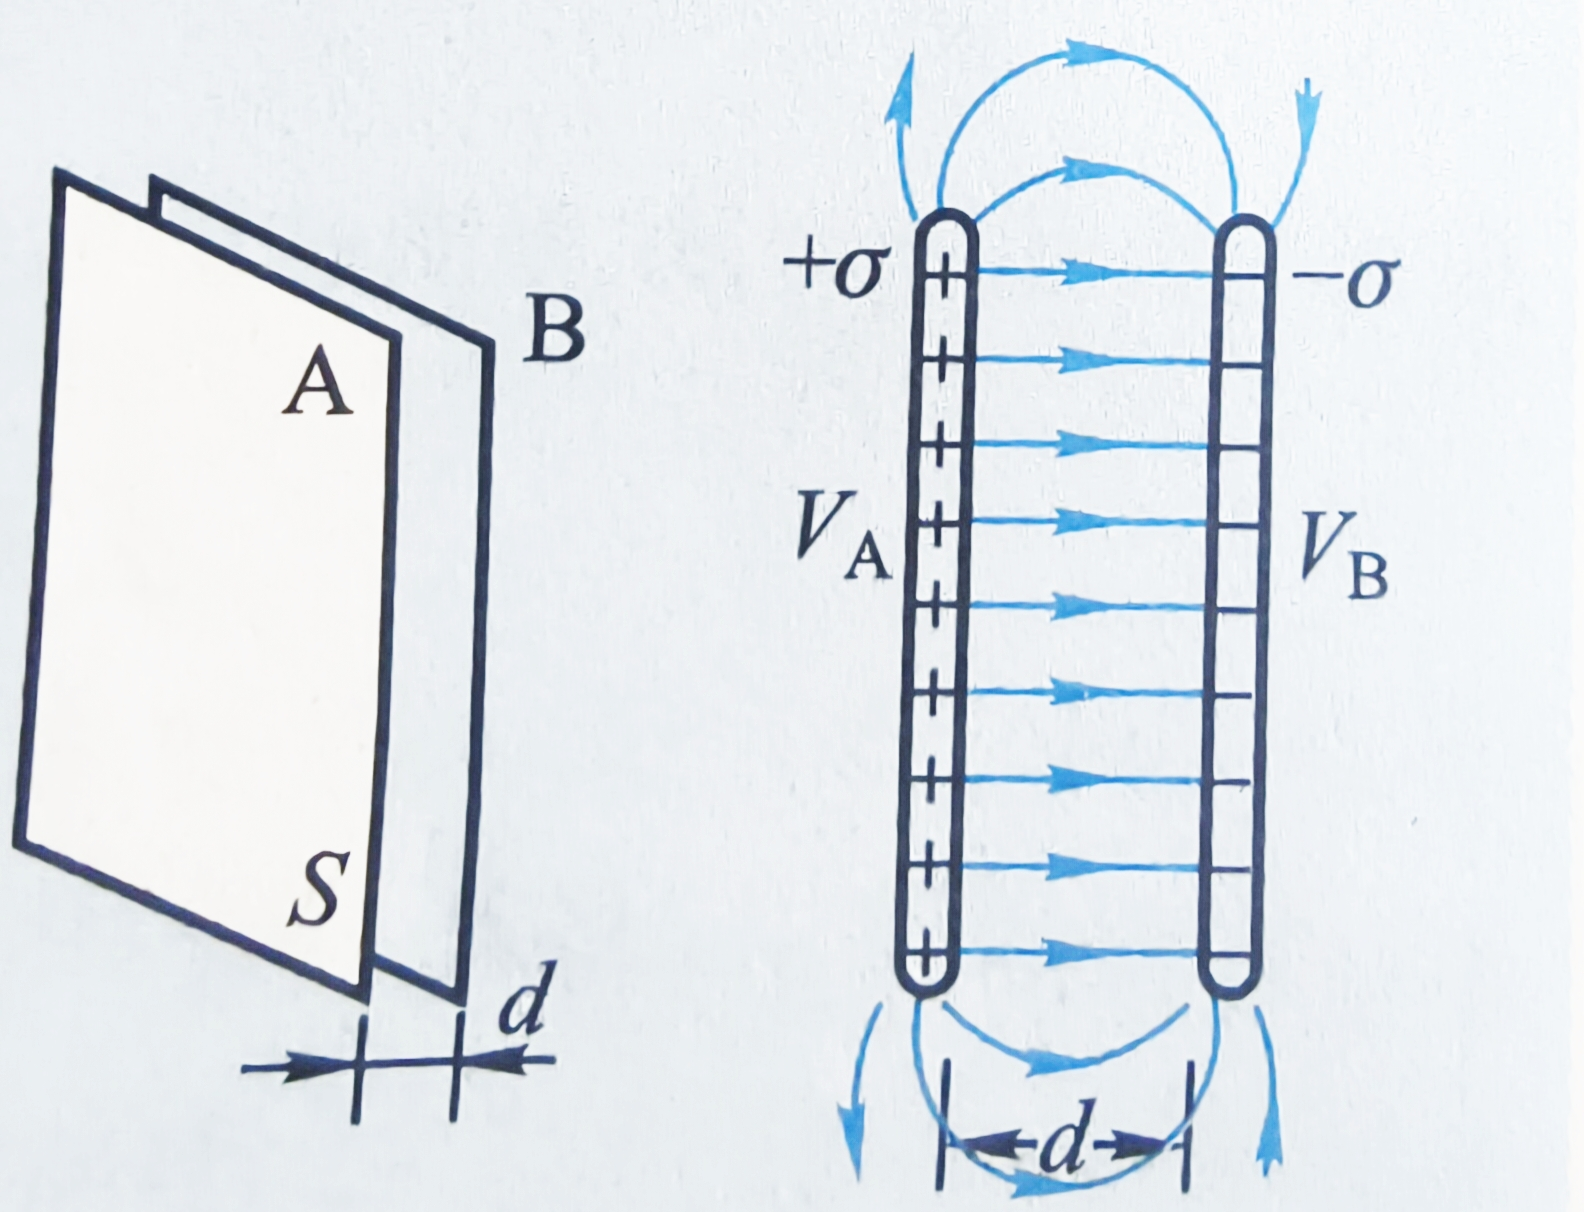
\includegraphics[width=0.4\linewidth]{images/平行板电容器}
	\caption{平行板电容器}
	\label{fig:}
\end{figure}

\subsubsection{同轴圆柱形电容器}

由于两极板距离很近，从两极板中间一点看，可以将其视作无限大带电平面，柱长为L，带电荷量为Q，内半径为$R_{A}$，外半径为$R_{B}$。

设线密度为$\lambda$，$\lambda =\frac{Q}{l}$

取圆柱形高斯面，半径为r,高度为h，则有$$\oint \mathbf{E}\mathrm{d}S=\int_{侧}\mathbf{E}\mathrm{d}S=2\mathbf{E}\pi rh=\frac{\lambda h}{\varepsilon_{0}}$$

求出$$\mathbf{E}=\frac{\lambda}{2\pi\varepsilon_{0}r} $$

则有$$U_{AB}=\int_{R_{A}}^{R_{B}}\mathbf{E}\mathrm{d}r=\int_{R_{A}}^{R_{B}}\frac{\lambda}{2\pi\varepsilon_{0}r}\mathrm{d}r=\frac{\lambda}{2\pi\varepsilon_{0}}\ln\frac{R_{B}}{R_{A}}$$
	
因此$$C=\frac{Q}{U_{AB}}=\frac{2\pi\varepsilon_{0}l}{\ln\frac{R_{B}}{R_{A}}}$$

\begin{figure}[h]
	\centering
	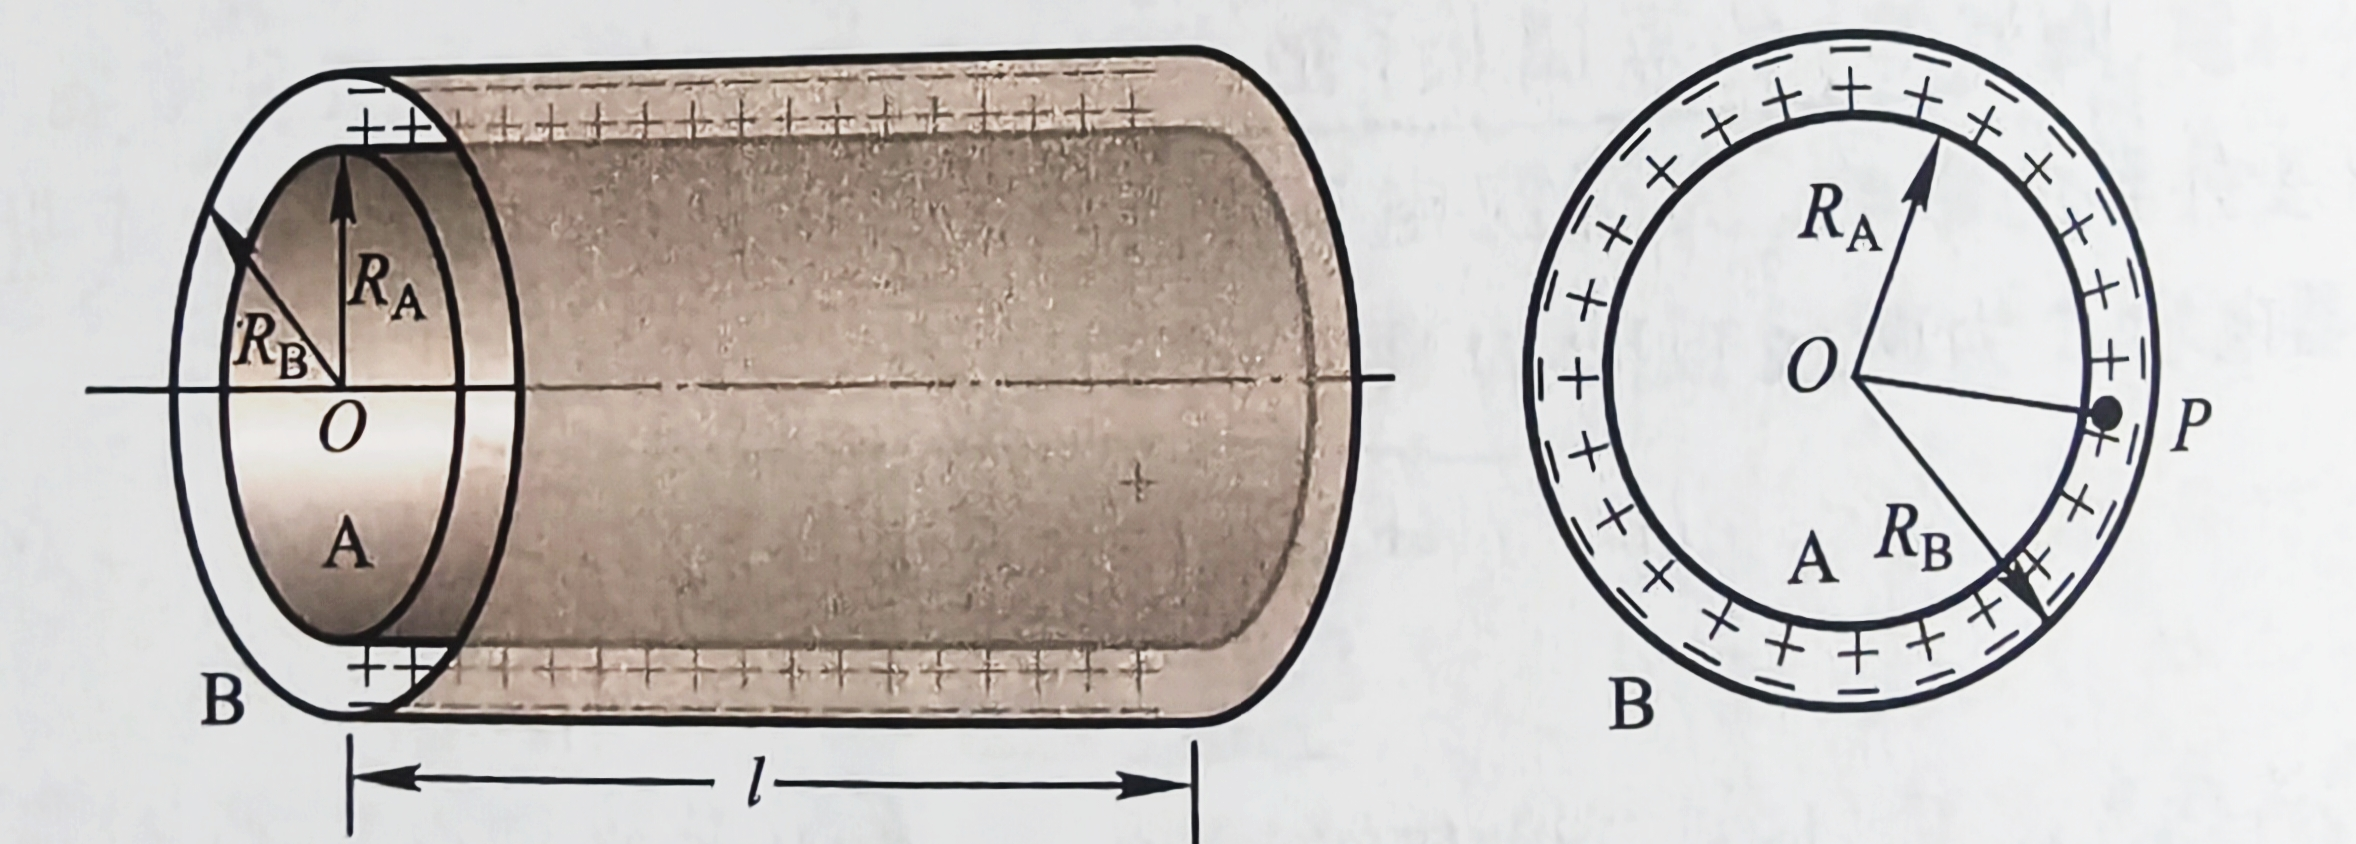
\includegraphics[width=0.5\linewidth]{images/同轴圆柱形电容器}
	\caption{同轴圆柱形电容器}
	\label{fig:}
\end{figure}

\subsubsection{球形电容器}

球形电容器由两个同心的金属球壳组成，内球面半径为$R_{A}$，外球面半径为$R_{B}$，带电荷量为Q。

当$R_{A}<r<R_{B}$时，$$\mathbf{E}=\frac{Q}{4\pi\varepsilon_{0}r^{2}}$$

则$$U_{AB}=V_{A}-V_{B}=\int_{R_{A}}^{R_{B}}\mathbf{E}\mathrm{d}r=\int_{R_{A}}^{R_{B}}\frac{Q}{4\pi\varepsilon_{0}r^{2}}\mathrm{d}r=\frac{Q}{4\pi\varepsilon_{0}}(\frac{1}{R_{A}}-\frac{1}{R_{B}})$$

则$$C=\frac{Q}{U_{AB}}=4\pi\varepsilon_{0}\frac{R_{A}R_{B}}{R_{B}-R_{A}}$$

\begin{figure}[h]
	\centering
	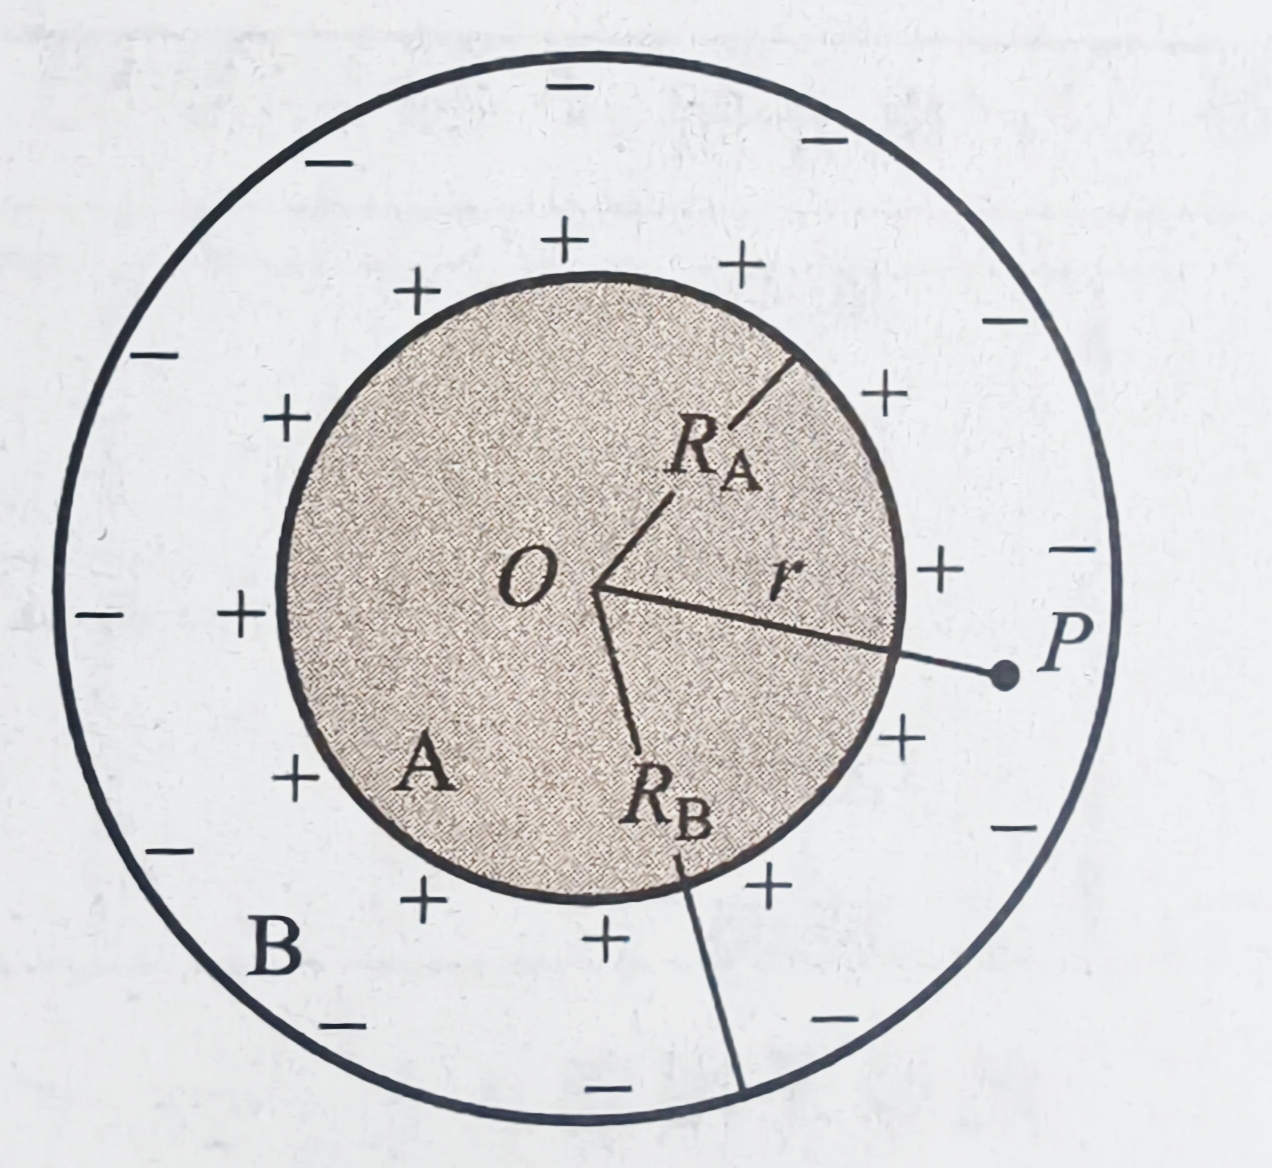
\includegraphics[width=0.4\linewidth]{images/球形电容器}
	\caption{球形电容器}
	\label{fig:}
\end{figure}

\subsection{电容器的串联与并联}

\subsubsection{电容器的串联}

$$C=\frac{Q}{U}=\frac{Q}{U_{1}+U_{2}+U_{3}+......+U_{n}}=\frac{Q}{\frac{Q}{C_{1}}+\frac{Q}{C_{2}}+\frac{Q}{C_{3}}+......+\frac{Q}{C_{n}}}=\frac{1}{\frac{1}{C_{1}}+\frac{1}{C_{2}}+\frac{1}{C_{3}}+......\frac{1}{C_{n}}} $$

\begin{figure}[h]
	\centering
	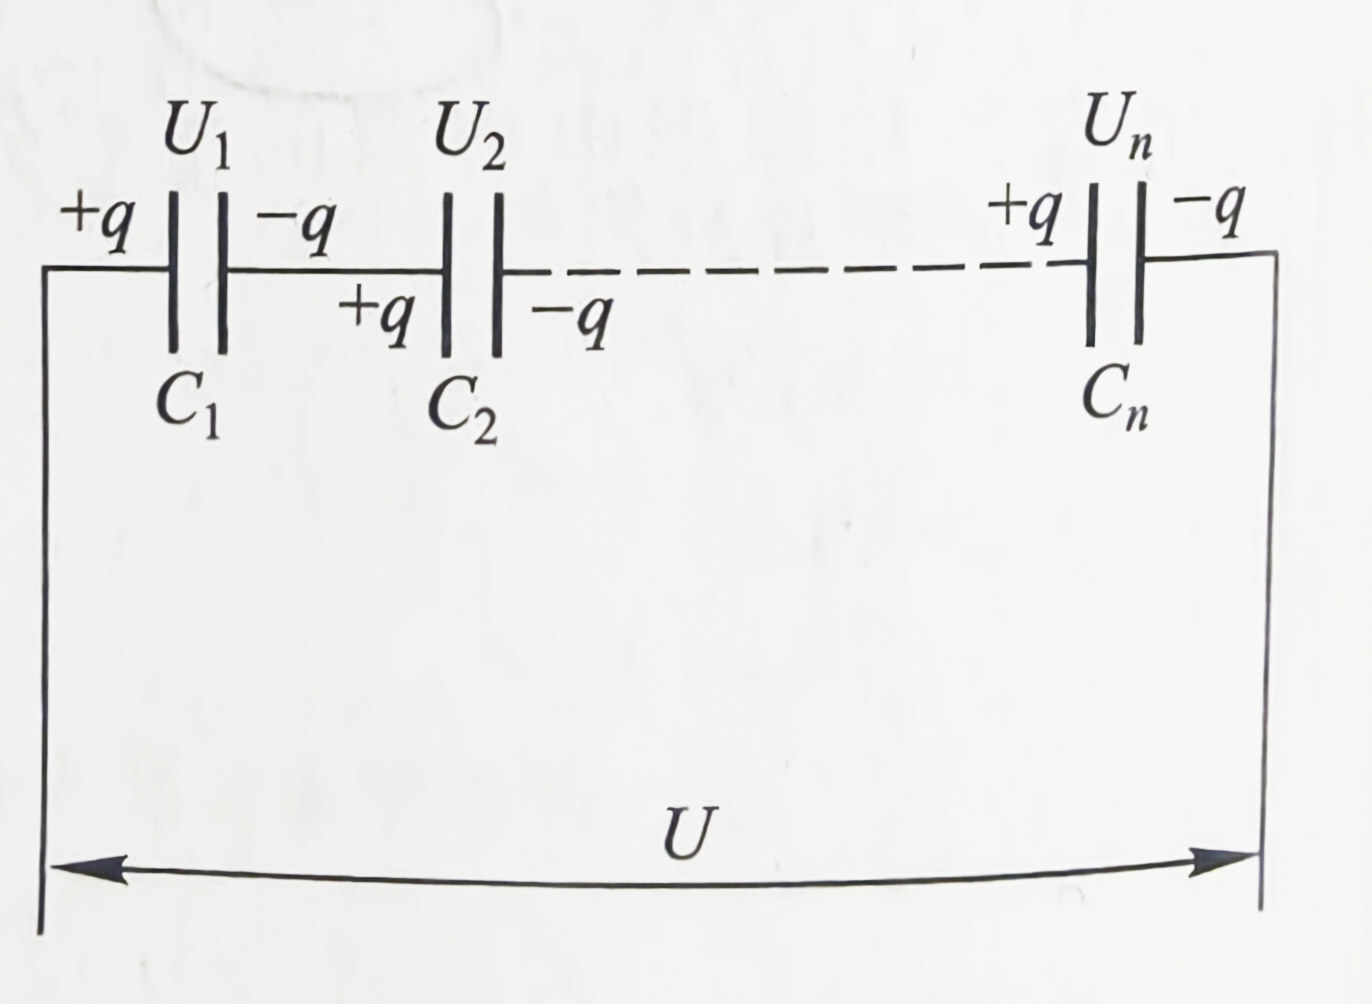
\includegraphics[width=0.4\linewidth]{images/电容器串联}
	\caption{电容器串联}
	\label{fig:}
\end{figure}

\subsubsection{电容器的并联}

$$C=\frac{Q}{U}=\frac{C_{1}U_{1}+C_{2}U_{2}+C_{3}U_{3}+......C_{n}U_{n}}{U} $$

\begin{figure}[h]
	\centering
	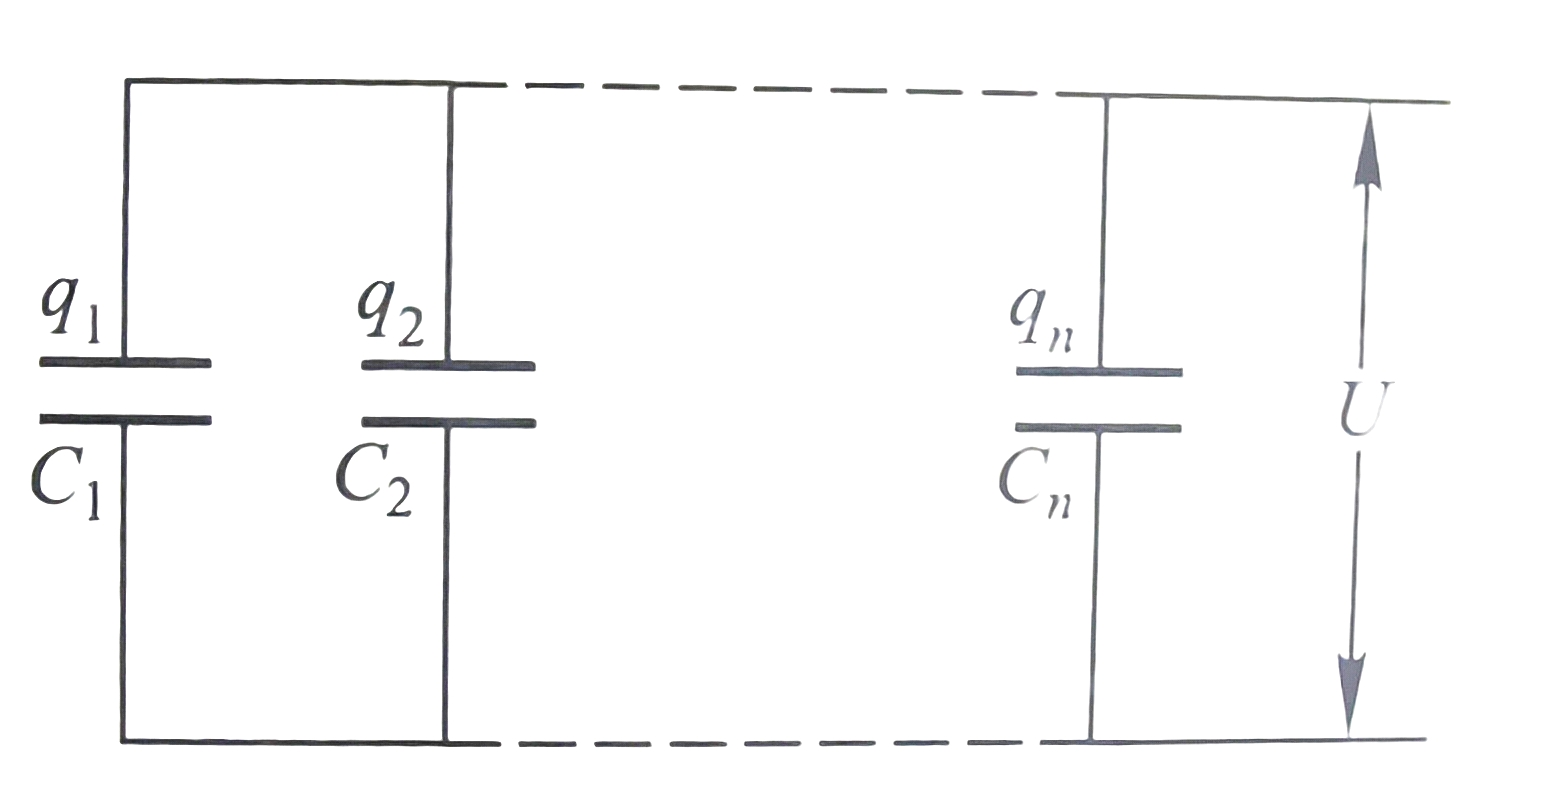
\includegraphics[width=0.5\linewidth]{images/电容器并联}
	\caption{电容器并联}
	\label{fig:}
\end{figure}

% \section{静电场中的电介质}
电介质的定义：电介质是电阻率很大，导电性能很差的物质。

电介质的极化：当电介质处在电场中时，电介质中，无论是原子中的电子还是分子中的离子或是晶体晶格上的带电粒子，在电场的作用下都会在原子大小的范围内移动。

当达到静电平衡时，在电介质表面层或体内会出现极化电荷，这个现象称作电介质的极化。

\subsection{电介质的电结构与极化}
\subsubsection{无极分子}
分子内正、负电荷中心重合，等效电偶极矩等于零，电介质整体呈电中性。

无极分子的极化来自正、负电荷中心的相对位移，所以常叫做位移极化。

\subsubsection{极性分子}
分子内正、负电荷中心不相重合。设极性分子的正负电荷中心之间的距离为$l$，分子中全部正电荷或负电荷的总电荷量为$q$，则等效电偶极矩$\vec{p}=q\vec{l}$，电介质整体呈电中性。

极性分子的极化就是等效电偶极子转向外电场的方向，叫做取向极化（一般来说，分子在取向极化的同时还会产生位移极化，但极性分子电介质以取向极化为主）。

\subsubsection{极化后电介质中的电荷分布}
如果电介质是均匀的，则在它内部仍然保持电中性，但是在电介质的两个和外电场强度$\vec{E_0}$相垂直的表面层里（厚度为分子等效电偶极矩的轴长$l$），将会分别出现正电荷和负电荷。

\subsection{电极化强度}
两类电介质极化的微观过程虽然不同，但宏观的效果却是相同的。都是在电介质的两个相对表面上出现了异号的极化电荷，在电介质内部有沿电场方向的电偶极矩。

我们取单位体积内分子电偶极矩的矢量和，即
$$\vec{P}=\frac{\sum \vec{p}}{\Delta V}$$
作为量度电介质极化程度的基本物理量，称为该点的电极化强度或$\vec{P}$矢量。单位是$C/m^2$。

\subsection{电极化强度与极化电荷的关系}
对于均匀电介质，其极化电荷只集中在表面层里或在两种不同的界面层里。

设$\vec{e_n}$为介质表面的单位法向矢量，那么
$$\sigma'=\vec{P}\cdot\vec{e_n}=P_n$$
即介质极化所产生的极化电荷面密度等于电极化强度沿介质表面外法线的分量。

\subsection{介质中的静电场}
\subsubsection{物理量}
电介质的电极化率：$\chi_e$，和电介质的性质有关，量纲为1。

电介质的相对电容率：$\varepsilon_r$

电介质的电容率/介电常量：$\varepsilon$

\subsubsection{公式}
对于各向同性电介质，有：

$\vec{E}=\vec{E_0}+\vec{E'}$

$\vec{P}=\chi_e\varepsilon_0\vec{E}$

$\varepsilon_r=1+\chi_e$

$\varepsilon=\varepsilon_r\varepsilon_0=(1+\chi_e)\varepsilon_0$

\subsubsection{（特例：平行板电容器）}
除满足以上公式外，还有

$E_0=\sigma_0/\varepsilon_0$

$E'=\sigma'/\varepsilon_0$

$E=\frac{E_0}{1+\chi_e}$

\subsubsection{拓展：非各向同性电介质}
自然界也存在一些电介质，在一定的温度范围内电容率随电场强度而变化，它们的极化规律有着复杂的线性关系。

如铁电体、永驻体、压电效应、电致伸缩等。
% 
	
	
	\section{有电介质时的高斯定理和环路定理  电位移}
	
	
	\begin{definition}[电位移]
		电位移用$D$表示，单位是$C/m^2$。
		$$D = \varepsilon_{0}E + P$$
		其中，$P$为电极化强度。
	\end{definition}
	
\begin{definition}[电位移通量]
在有电介质的静电场中作电位移线，使线上每一点的切线方向和该点电位移 D 的方向相同，并规定在垂直于电位移线的单位面积上通过的电位移线数目等于该点的电位移 D 的量值，被称为称作电位移通量。
\end{definition}
	
	\begin{definition}[有电介质时的高斯定理]
		$$\oint_{S} D \cdot dS = q_{0}$$
	\end{definition}
	
\begin{note}
有电介质时的高斯定理是静电场基本定理之一，是普遍适用的。
	
通过电介质中任一闭合曲面的电位移通量，等于该面所包围的自由电荷量的代数和。

电位移线是从正的自由电荷出发，终止于负的自由电荷（不包括极化电荷）。

\end{note}
	
	
\begin{note}
$D$和$E$和$P$的关系和区分：

有电介质时，平行板电容器之间$D$线均匀分布（从正的自由电荷出发，终止于负的自由电荷）（不包括极化电荷），$E$线有部分终止于极化电荷，在电介质内较为疏松，$P$线起始于负极化电荷，终止于正极化电荷，只在电介质内部。

设电极化率为$\chi_{e}$，相对电容率$\varepsilon_{0}$，电容率$\varepsilon$
$$D = \varepsilon_{0}E + P = \varepsilon_{0}E + \chi_{e}\varepsilon_{0}E = \varepsilon_{r}\varepsilon_{0}E$$
	$$D = \varepsilon E$$
		
\end{note}
	
	\begin{definition}[有电介质时的环路定理]
$$\oint_{L} E \cdot dl = 0$$
$E$为所有电荷激发的静电场。
	\end{definition}
\begin{supplement}
带电金属球周围充满均匀无限大电介质后，其电场强度减弱到真空时的$\frac{1}{\varepsilon_{r}}$
\end{supplement}

\begin{supplement}
$E = \frac{E_{0} }{\varepsilon_{r}}$ 和 $D = \varepsilon_{0}E $仅在均匀电介质充满整个电场或电介质表面是等势面时成立。
\end{supplement}
	

	

% \chapter{静磁场}
\section{毕奥-萨伐尔定律}
\subsection{毕奥-萨伐尔定律}
电流元$I\mathbf{d}\vec{l}$在空间任一点P处所激发磁场的磁感应强度为
$$\mathbf{d}\vec{B}=\frac{\mu_0}{4\pi}\frac{I\mathbf{d}\vec{l}\times\vec{e_r}}{r^2}$$

电流元：用矢量$I\mathbf{d}\vec{l}$表示。其中$\mathbf{d}\vec{l}$表示在载流导线上（沿电流方向）所取的线元，$I$为导线中的电流，电流元的方向规定为电流沿线元的流向。

$\mu_0=4\pi\times10^{-7}T\cdot m/A$，称为真空磁导率。

$\vec{e_r}$是从电流元所在处到场点$P$的位矢。

\subsection{应用示例}
\subsubsection{载流直导线}
对于长为$L$的载流直导线，距离直导线为$a$的$P$点的磁感应强度：
$$B=\frac{\mu_0 I}{4\pi a}(\sin\beta_2-\sin\beta_1)$$
\begin{figure}[h]
	\centering
	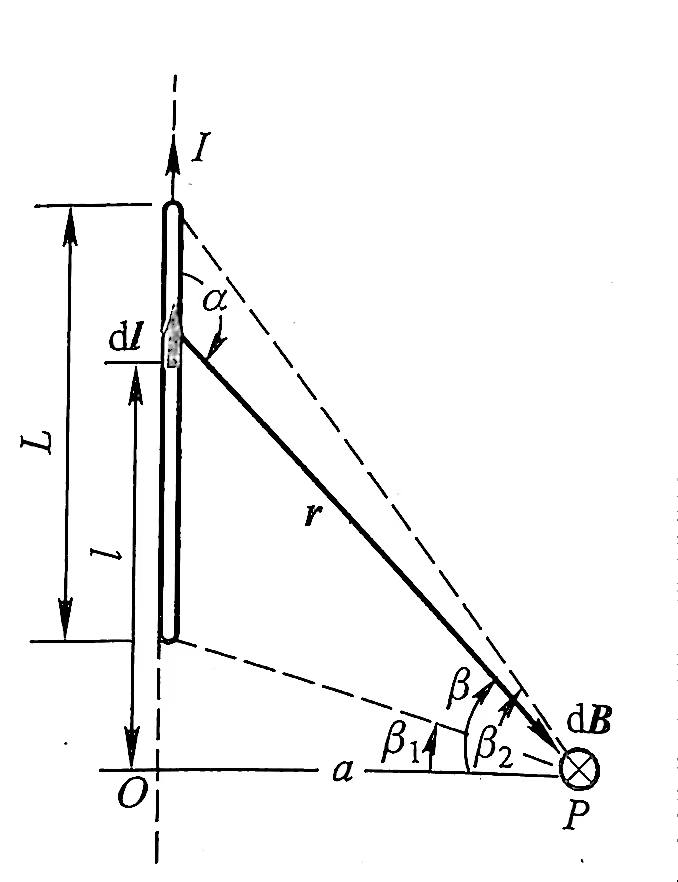
\includegraphics[width=0.3\textwidth]{images/8.3 载流直导线.jpg}
	\caption{载流直导线附近磁场的计算}
\end{figure}

对于无限长载流直导线，取$\beta_1=-\pi/2$，$\beta_2=\pi/2$，得：
$$B=\frac{\mu_0 I}{2\pi a}$$

\subsubsection{载流圆线圈的轴线}
$$B=\frac{\mu_0}{2\pi}\frac{IS}{(R^2+x^2)^{3/2}}$$
\begin{figure}[h]
	\centering
	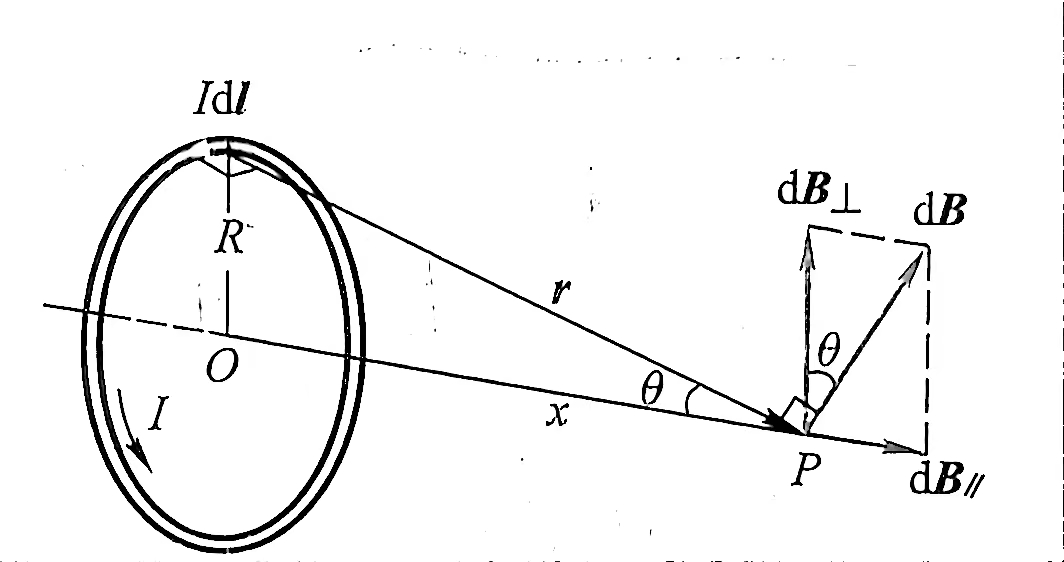
\includegraphics[width=0.5\textwidth]{images/8.3 圆电流轴线.jpg}
	\caption{圆电流轴线上磁场的计算}
\end{figure}

在圆心$x=0$处，$B_0=\frac{\mu_0I}{2R}$

当$x\gg R$时，$B=\frac{\mu_0IS}{2\pi x^3}$

引入磁矩$\vec{m}=IS\vec{e_n}$（若线圈有$N$匝，则磁场加强$N$倍，$\vec{m}=NIS\vec{e_n}$），其中$\vec{e_n}$表示线圈平面法线方向的单位矢量（由线圈中电流流向按右手螺旋定则确定）。则：
$$\vec{B}=\frac{\mu_0\vec{m}}{2\pi x^3}$$
\begin{figure}[h]
	\centering
	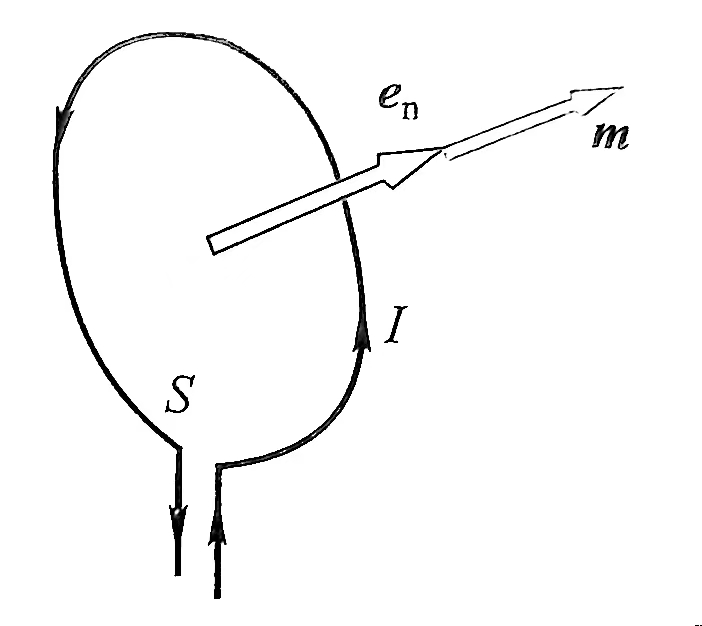
\includegraphics[width=0.3\textwidth]{images/8.3 磁矩.jpg}
	\caption{磁矩的方向}
\end{figure}

\subsubsection{载流直螺管内部}
\begin{figure}[h]
	\centering
	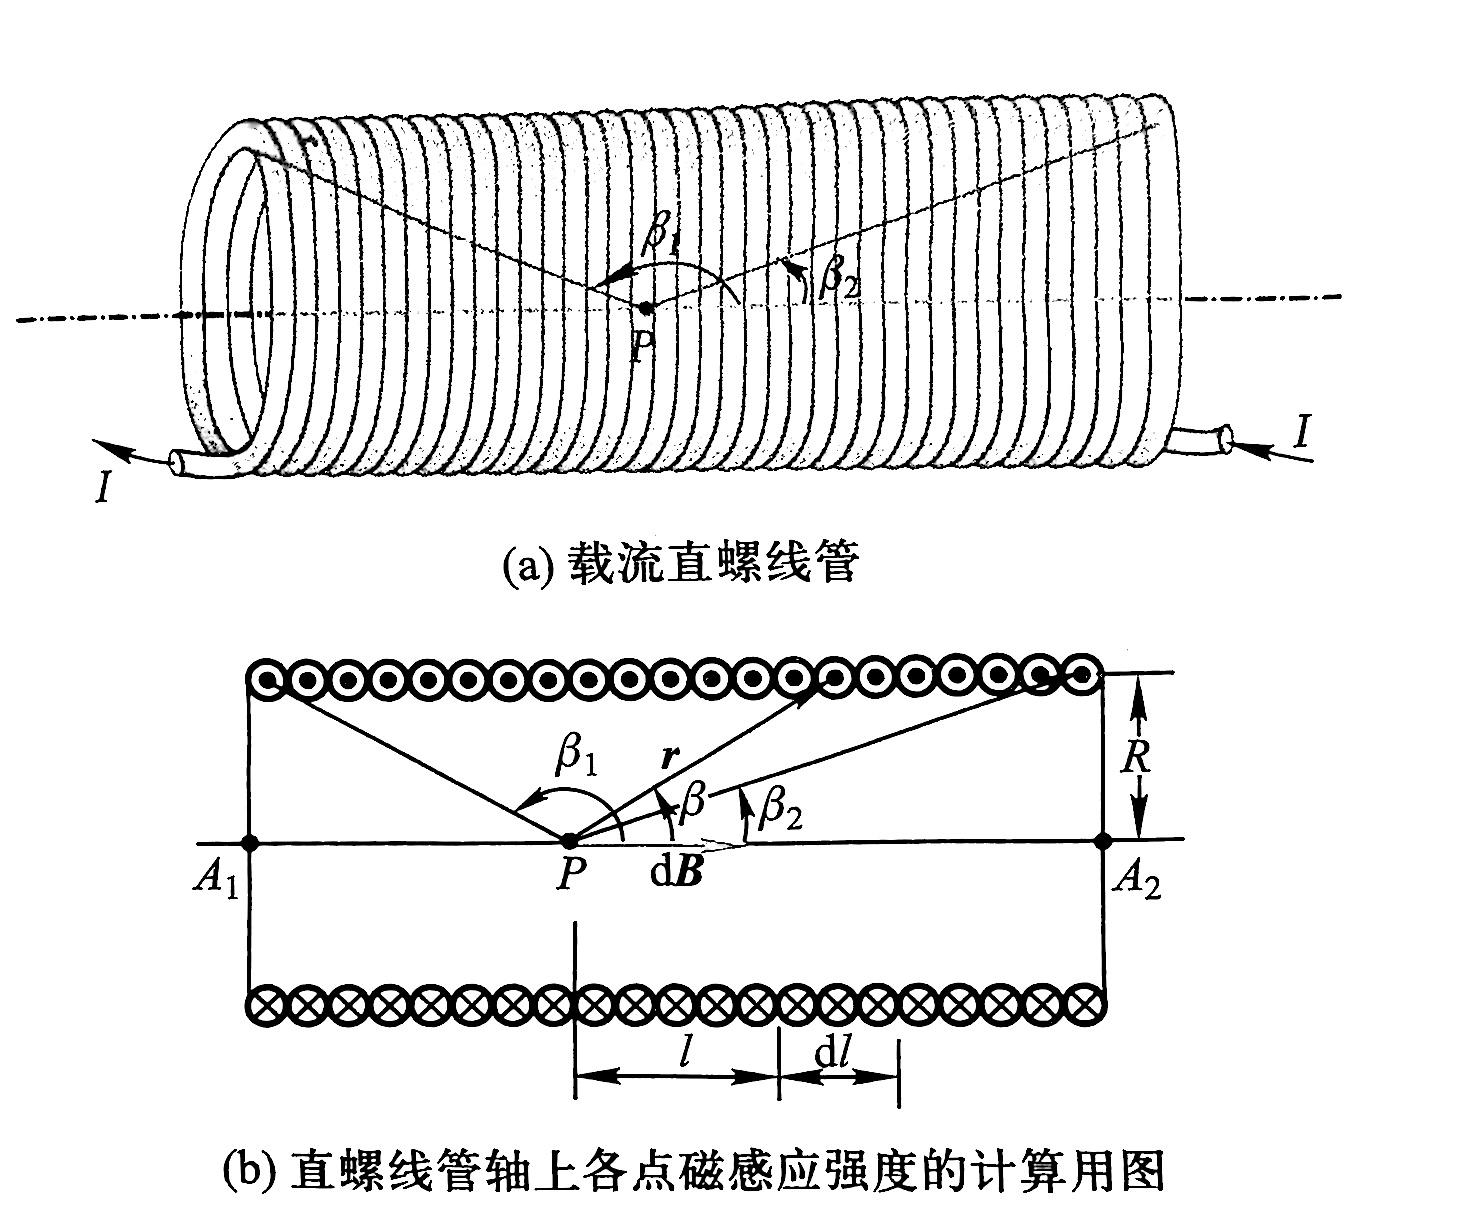
\includegraphics[width=0.5\textwidth]{images/8.3 直螺线管内部.jpg}
	\caption{直螺线管内部磁场的计算}
\end{figure}
螺线管半径为$R$，电流为$I$，每单位长度有线圈$n$匝：
$$B=\frac{\mu_0}{2}nI(\cos\beta_2-\cos\beta_1)$$

无限长螺线管，亦即螺线管的长度$\gg$其直径时：
$$B=\mu_0 nI$$

长螺线管的端点：
$$B=\frac{1}{2}\mu_0 nI$$

\subsection{运动电荷的磁场}
每一个以速度$v$运动的电荷所激发磁场的磁感应强度$B_q$为：
$$B_q=\frac{\mu_0}{4\pi}\frac{q\vec{v}\times\vec{e_r}}{r^2}$$
% \section{恒定磁场的高斯定理与安培环路定理}

\subsection{恒定磁场的高斯定理}

1.\textbf{通过任意闭合曲面的磁通量总等于零。}
即$$\oint_{S}\mathbf{B}\mathrm{d}S=0$$

2.激发静电场的场源（电荷）是电场线的源头或尾闾，所以静电场是属于发散状的场，可称作有源场；而磁场的磁感应线无头无尾，永远是闭合的，所以磁场可称作无源场。

3.磁场的高斯定理与静电场的高斯定理不对称的根本原因是自然界不存在单
个磁极（即磁单极子）。

\subsection{恒定磁场的安培环路定理}

1.\textbf{在恒定磁场中，磁感应强度治任一闭合路径的线积分等于$\mu_{0}$倍的穿过以闭合曲线为边界的任意曲面的各恒定电流的代数和,也称为矢量的环流}
即$$\oint\mathbf{B}\mathrm{d}\mathbf{l}=\mu_{0}\sum I_{i}$$

2.通常把磁场叫做有旋场，而$\mathbf{E}$的环流恒等于零，所以把静电场叫做无旋场。

3.讨论:

(1)B是空间全部电流产生的磁场。

(2)对任意形式的恒定电流所激发的磁场都成立，对任何形形状的闭合路径都成立。

\subsection{典型安培环路定理的应用}

\subsubsection{无限长直电流的磁场}

\begin{figure}[h]
	\centering
	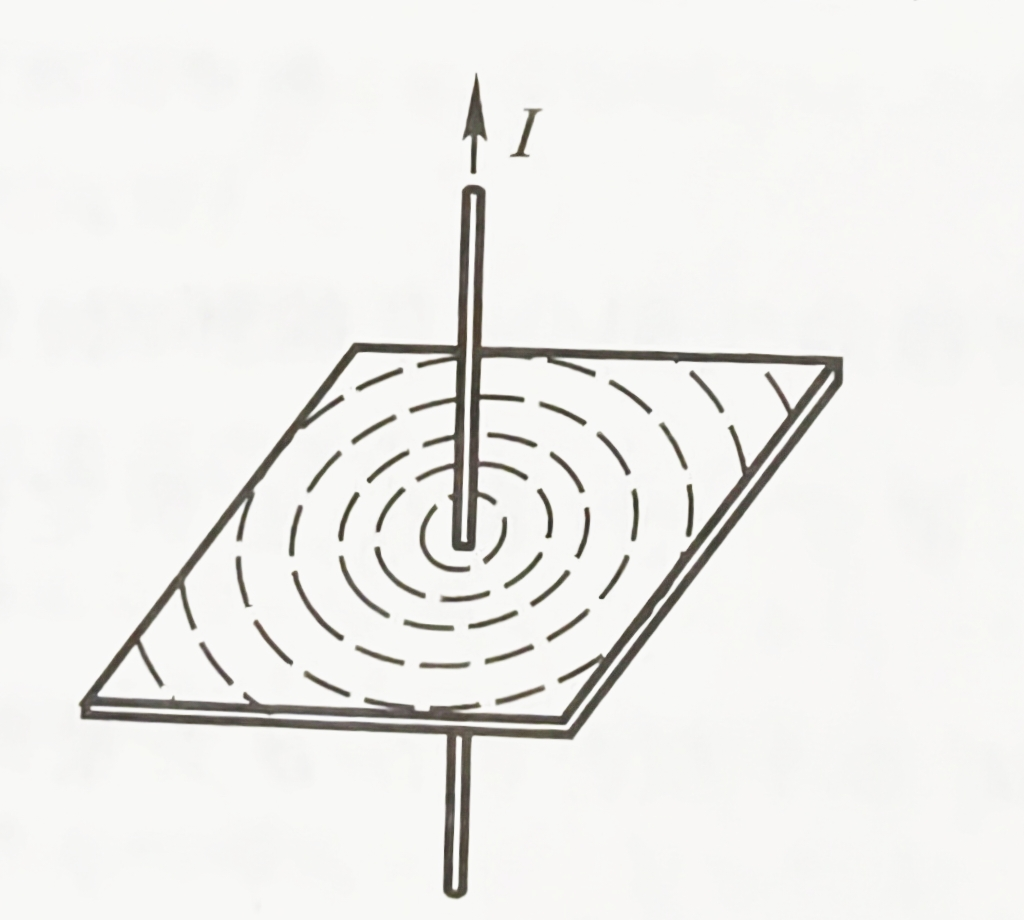
\includegraphics[width=0.4\linewidth]{images/无限长直导线的磁场}
	\caption{无限长直导线的磁场}
	\label{fig:}
\end{figure}

磁场为一圈一圈的同心圆，取闭合路径为磁场的同心圆，半径为r。

由安培环路定理$$ \oint\mathbf{B}\mathrm{d}\mathbf{l}=\oint B\mathrm{d}l=B\oint\mathrm{d}l=\mu_{0}\sum I_{i}$$

则$$2B\pi r=\mu_{0}I$$
$$B=\frac{\mu_{0}I}{2\pi r}$$

方向与电流流向呈右手螺旋定则

\subsubsection{长直圆柱形载流导线内外的磁场}

\begin{figure}[h]
	\centering
	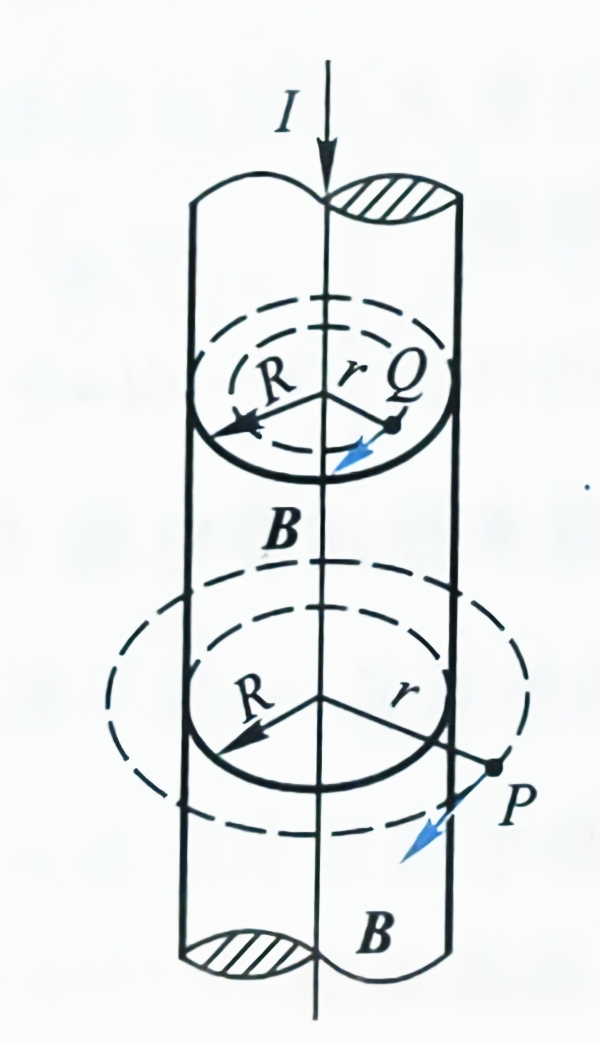
\includegraphics[width=0.2\linewidth]{images/长直圆柱形载流导线内外的磁场}
	\caption{长直圆柱形载流导线内外的磁场}
	\label{fig:}
\end{figure}

从轴线方向看，上下左右对称的电流对圆柱形载流导线外一点的磁感应强度是对称的，因此磁场呈轴对称分布，磁感应线为垂直于轴线的同心圆。

圆柱的半径为R，取半径为r的同心圆为闭合路径。

则由安培环路定理$$\oint\mathbf{B}\mathrm{d}\mathbf{l}=\oint B\mathrm{d}l=B\oint\mathrm{d}l=\mu_{0}\sum I_{i} $$

1.当r>R时，则$$2B\pi r=\mu_{0}I$$

2.当r<R时，则$$2B\pi r=\mu_{0}\frac{\pi r^{2}}{\pi R_{^{2}}}$$

则$$\left\{
\begin{aligned}
	B&=\frac{\mu_{0}I}{2\pi r}，,r>R\\
	B&=\frac{\mu_{0}Ir}{2\pi R}，,r<R
\end{aligned}
\right.$$

\subsubsection{均匀密绕无限长直螺线管的磁场}

\begin{figure}[h]
	\centering
	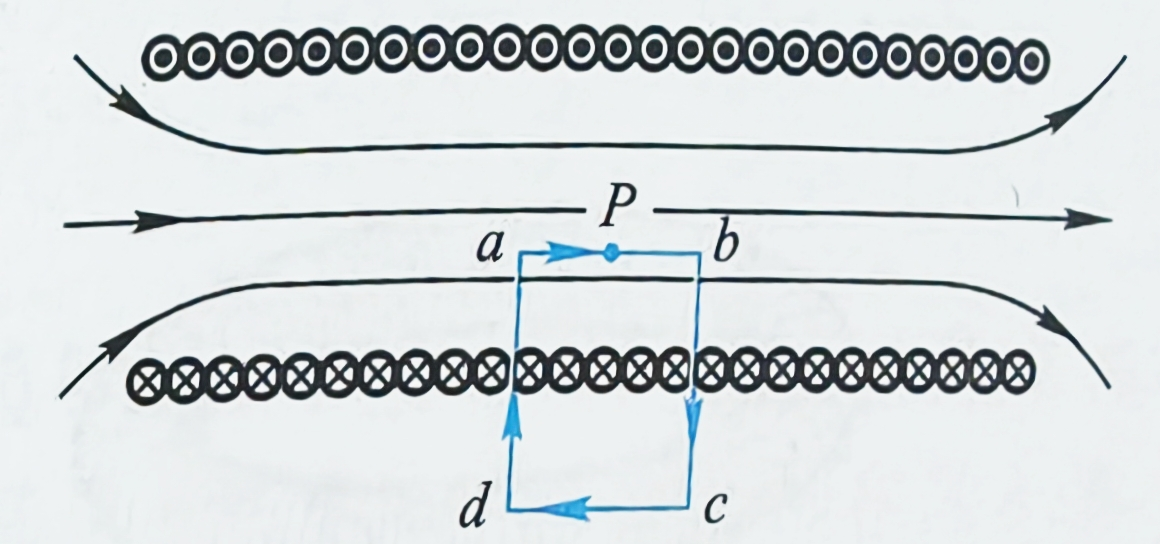
\includegraphics[width=0.5\linewidth]{images/均匀密绕无限长直螺线管的磁场}
	\caption{均匀密绕无限长直螺线管的磁场}
	\label{fig:}
\end{figure}

已知有N匝线圈，电流为I，数密度为n。

P为螺线管内一点，由分析可知，P点磁感线的方向为过点P且平行于轴线的方向，该同一直线上其他点方向也沿该直线。即\textbf{P点所在的平行直线上大小相同，方向相同}

取闭合回路为矩形abcda

则由安培环路定理$$\oint\mathbf{B}\mathrm{d}\mathbf{l}=Bl_{ab}=\mu_{0}nl_{ab}I$$

则$$B=\mu_{0}nI $$

在螺线管外部，磁感线相互抵消，磁感应强度很小，$B_{内}\gg B_{外}$，可视做$B_{外}=0 $，所以多匝线圈一般被视为储能原件。

\subsubsection{均匀载流螺绕环的磁场}

\begin{figure}[h]
	\centering
	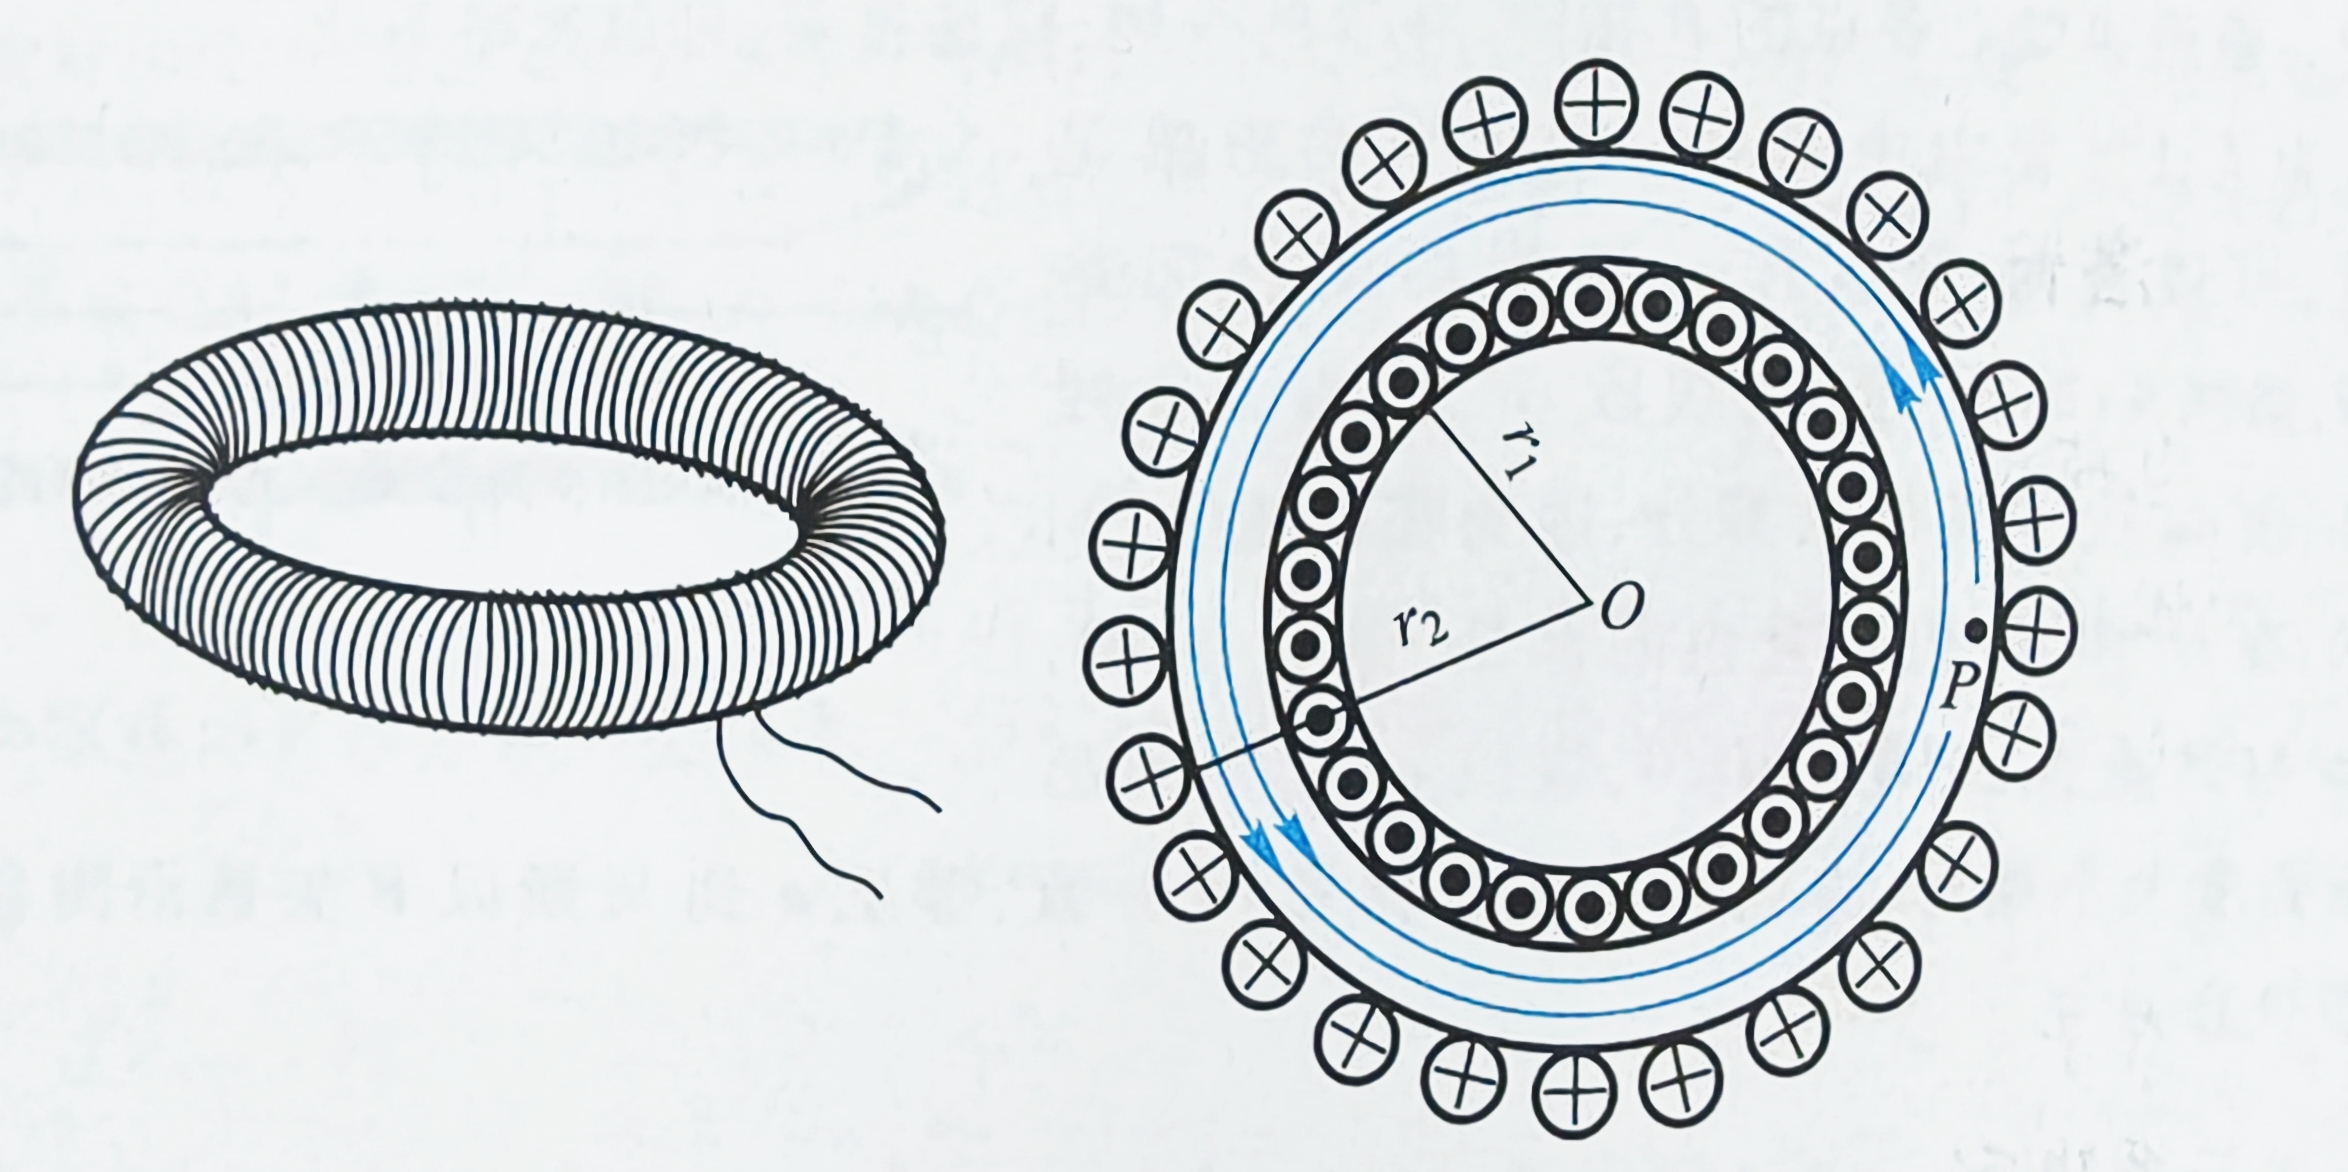
\includegraphics[width=0.6\linewidth]{images/均匀载流螺绕环的磁场}
	\caption{}
	\label{fig:}
\end{figure}

已知内径为$R_{1}$，外径为$R_{2}$，电流为I，匝数为N。

经放大图分析，螺绕环的磁感线为其内部的同心圆，取半径为r的同心圆为闭合路径。

则由安培环路定理$$\oint\mathbf{B}\mathrm{d}\mathbf{l}=\oint B\mathrm{d}l=B\oint\mathrm{d}l=\mu_{0}\sum I_{i} $$

1.当$R_{1}$<r<$R_{2}$时，则$$2B\pi r=\mu_{0}NI$$

2.当r>$R_{2}$时，电流相互抵消，则$$2B\pi r=0$$

则$$\left\{
\begin{aligned}
	B&=\frac{\mu_{0}NI}{2\pi r},R_{1}<r<R_{2}\\
	B&=0,r>R_{2}
\end{aligned}
\right.$$
% \section{铁磁质}
概括起来说，铁磁质有下列一些特殊的性质：
\begin{enumerate}
	\item 能产生特别强的附加磁场$B'$，使铁磁质中的$B$远大于$B_0$,其$\mu_r=B/B_0$可达几百、甚至几千。
	\item 它们的磁化强度$M$和磁感应强度$B$不再是常矢量，没有简单的正比关系，其磁导率$\mu$（以及磁化率$\chi_m$）与磁场强度$H$的函数关系比较复杂。
	\item 磁化强度随外磁场而变，它的变化落后于外磁场的变化，而且在外磁场停止作用后，铁磁质仍能保留部分磁性。
	\item 一些铁磁质存在一特定的临界温度，称为居里点（Curie point)，在温度达到居里点后，它们的磁性发生突变，转化为顺磁质，磁导率（或磁化率）和磁场强度$H$无关。例如，铁的居里点是1040$K$，镍的是631$K$，钻的是1388$K$。
\end{enumerate}
% \chapter{电磁感应}
\section{磁场的能量}
\subsection{推导}
设电路接通后回路中某瞬时的电流为$I$，自感电动势为$-L\mathbf{d}I/\mathbf{d}t$，由回路的欧姆定律得
$$\varepsilon-L\frac{\mathbf{d}I}{\mathbf{d}t}=IR$$
$$\int_{0}^{t}\varepsilon I\mathbf{d}t=\int_{0}^{I_0}LI\mathbf{d}I+\int_{0}^{t}R^2I^2\mathbf{d}I$$

在自感与电流无关的情况下，得到
$$\int_{0}^{t}\varepsilon I\mathbf{d}t=\frac{1}{2}LI_0^2+\int_{0}^{t}R^2I^2\mathbf{d}I$$

说明电源电动势所做的功转化为两部分能量。其中$\int_{0}^{t}R^2I^2\mathbf{d}I$是$t$时间内消耗在电阻$R$上的焦耳热；$\frac{1}{2}LI_0^2$是回路中建立电流的变化过程中电源电动势克服自感电动势所做的功，也就是储存在磁场中的能量。
\subsection{结论}
\subsubsection{磁场的能量}
一个自感为$L$的回路，当其中通有电流$I_0$时，其周围空间磁场的能量为
$$W_m=\frac{1}{2}LI_0^2$$

\subsubsection{磁场能量密度}
在一般情况下，磁场能量密度可以表达为
$$w_e=\frac{1}{2}\vec{B}\cdot\vec{H}$$

若磁场是不均匀的，则：
$$W_m=\int_{V}w_m\mathbf{d}V=\frac{1}{2}\int_{V}\vec{B}\cdot\vec{H}\mathbf{d}V$$

由$\frac{1}{2}LI_0^2=\frac{1}{2}\int_{V}\vec{B}\cdot\vec{H}\mathbf{d}V$，可求出回路的自感。

\end{document}
